\chapter[Climate Change]{Climate Change and Future Unimpaired Flow} \label{ch5:climatechange}
\chaptermark{Climate Change}
\setlength{\epigraphwidth}{5.5in}
\epigraph{For all of its uncertainty we cannot flee the future.}{Barbara Jordan, \textit{``Democratic National Convention Keynote Address''}, 1976}

%----------------------------------------------------------------------------------------------------------------------------------------------------------------------------------------------------------
\section*{Summary}
Future water resources conditions are usually estimated using projected climate variables (i.e., precipitation and temperature) from global climate models (GCMs) and a hydrologic model that routes precipitation to runoff. \citeA{pierce2018climate} identify a subset of four, out of the 32, GCMs that have done particularly well reproducing California's historical climate and are recommended when using more GCM data is prohibitive. In this chapter, these models each with two RCPs (4.5 and 8.5), are used to study future hydrology. \citeA{pierce2018climate} bias-corrected and downscaled the GCM data using the Localized Constructed Analogues (LOCA) statistical method. The downscaled runoff was then aggregated to the CDEC basin boundaries as a simple routing technique for this dissertation. Each downscaled climate change model data is put through the NN model built on past hydrology and the model predictions are compared to the climate model projections. 

There is fairly good agreement in the statistical (NN) model's unimpaired flow predictions and the mechanistic (GCM) models' routed runoff (R\textsuperscript{2}= [0.65-0.72]). However, the NN model does not capture low flows like the climate models and overestimates their values so much that when we compare more smoothed data (with a moving average window) we can see a bias emerge (e.g., $\beta_1$= 0.95 to 1.84 for CanESM2 RCP 4.5). This can also be seen in the time series comparisons; with a larger moving average window, the NN model's predictions are consistently higher than the climate model projections. 

%----------------------------------------------------------------------------------------------------------------------------------------------------------------------------------------------------------
\section{Introduction}
Future water resources conditions are usually estimated using projected climate variables (i.e., precipitation and temperature) from global climate models (GCMs) and a hydrologic model that routes precipitation to runoff. A more robust climate assessment relies on multiple scenarios of future climate from current GCMs available. Two common Representative Concentration Pathways (RCPs) provide information on possible scenarios or development trajectories for the main forcing agents of climate change. RCPs encapsulate particular sets containing emission of aerosols, concentration of greenhouse gasses, and land-use trajectories. For example, RCP 4.5 is a ``medium'' stabilization emissions scenario that models a future where societies attempt to reduce greenhouse gas emissions, while RCP 8.5 is a very high baseline or ``business-as-usual'' emission scenario \cite{van2011representative}. 

The data used here originally came from the Climate Model Intercomparison Project version 5 (CMIP5; \citeNP{taylor2012overview}), which includes 32 coarse-resolution ($\sim$ 100 km) GCMs. The data were bias corrected and downscaled using the Localized Constructed Analogues (LOCA) statistical method to better capture key features in California's climate \cite{pierce2018climate}. These data are available at www.caladapt.org and can be downloaded with a simple {\tt Rcurl} script and the CalAdapt API. 

Differences in climate change projections from different climate models arises from: (1) model uncertainty: inexact and differing representation of various processes, (2) scenario uncertainty: unknown rates and changes in climate forcings (e.g., rate and concentration of CO\textsubscript{2} and other greenhouse gases), and (3) climate uncertainty: unknown  internal variability of the climate such as El Niño \cite{hawkins2011potential}. \citeA{pierce2018climate} identifies a subset of four, out of 32, GCMs that have done particularly well reproducing California's historical climate and are recommended when using more GCM data is prohibitive. In this chapter, the following models, each with two RCPs (4.5 and 8.5), are used to explore future hydrology:

\begin{itemize}
	\item CanESM2 (CCCma, BC, Canada): an ``average'' model in terms of changes in precipitation and temperature.
	\item CNRM\-CM5 (CNRM and CERFACS, Toulouse, France): a ``cool/wet'' model. %, but, is merely less warm/dry than others.
	\item HadGEM2\-ES (Met Office Hadley Centre, UK): a ``warm/dry'' model.
	\item MIROC5 (JAMSTEC, AORI, and NIES, Japan): a model most unlike the other three.
\end{itemize}

%----------------------------------------------------------------------------------------------------------------------------------------------------------------------------------------------------------
\section{Climate Change Data}
Figures \ref{fig:rpdmap_ppt}, \ref{fig:rpdmap_tmp}, and \ref{fig:rpdmap_rnf} compare the relative percent difference (RPD) in precipitation, temperature, and runoff in the different climate models. To calculate RDP, first, the annual values are averaged across time in both the projected data (2015-2099) and the observed data (1914-2014). Then, the RDP is calculated using Equation \ref{eq:rpd}. Its value always lies between $-200$\% and $200$\%. It is positive when the mean projected data exceeds the mean observed and negative when the mean observed exceeds the mean projected. A regular percent difference was not calculated because dividing by zeros in the mean observed values creates large relative errors. 

\begin{equation}
	\label{eq:rpd}
	RPD(x, y) =2 \frac{x-y}{|x|+|y|} *100\% \quad\quad\text{RPD} \in $[-200\% , 200\%]$\\
\end{equation}

%compared climate model predictions against one another
%Annual rolling mean and sd plots

%\begin{figure}
%	\centering
%	\includegraphics[width=\textwidth,trim={0 0 0 0},clip=true]{plots/.png}
%	\caption[]{} 
%	\label{fig:}
%\end{figure}

\begin{figure}
    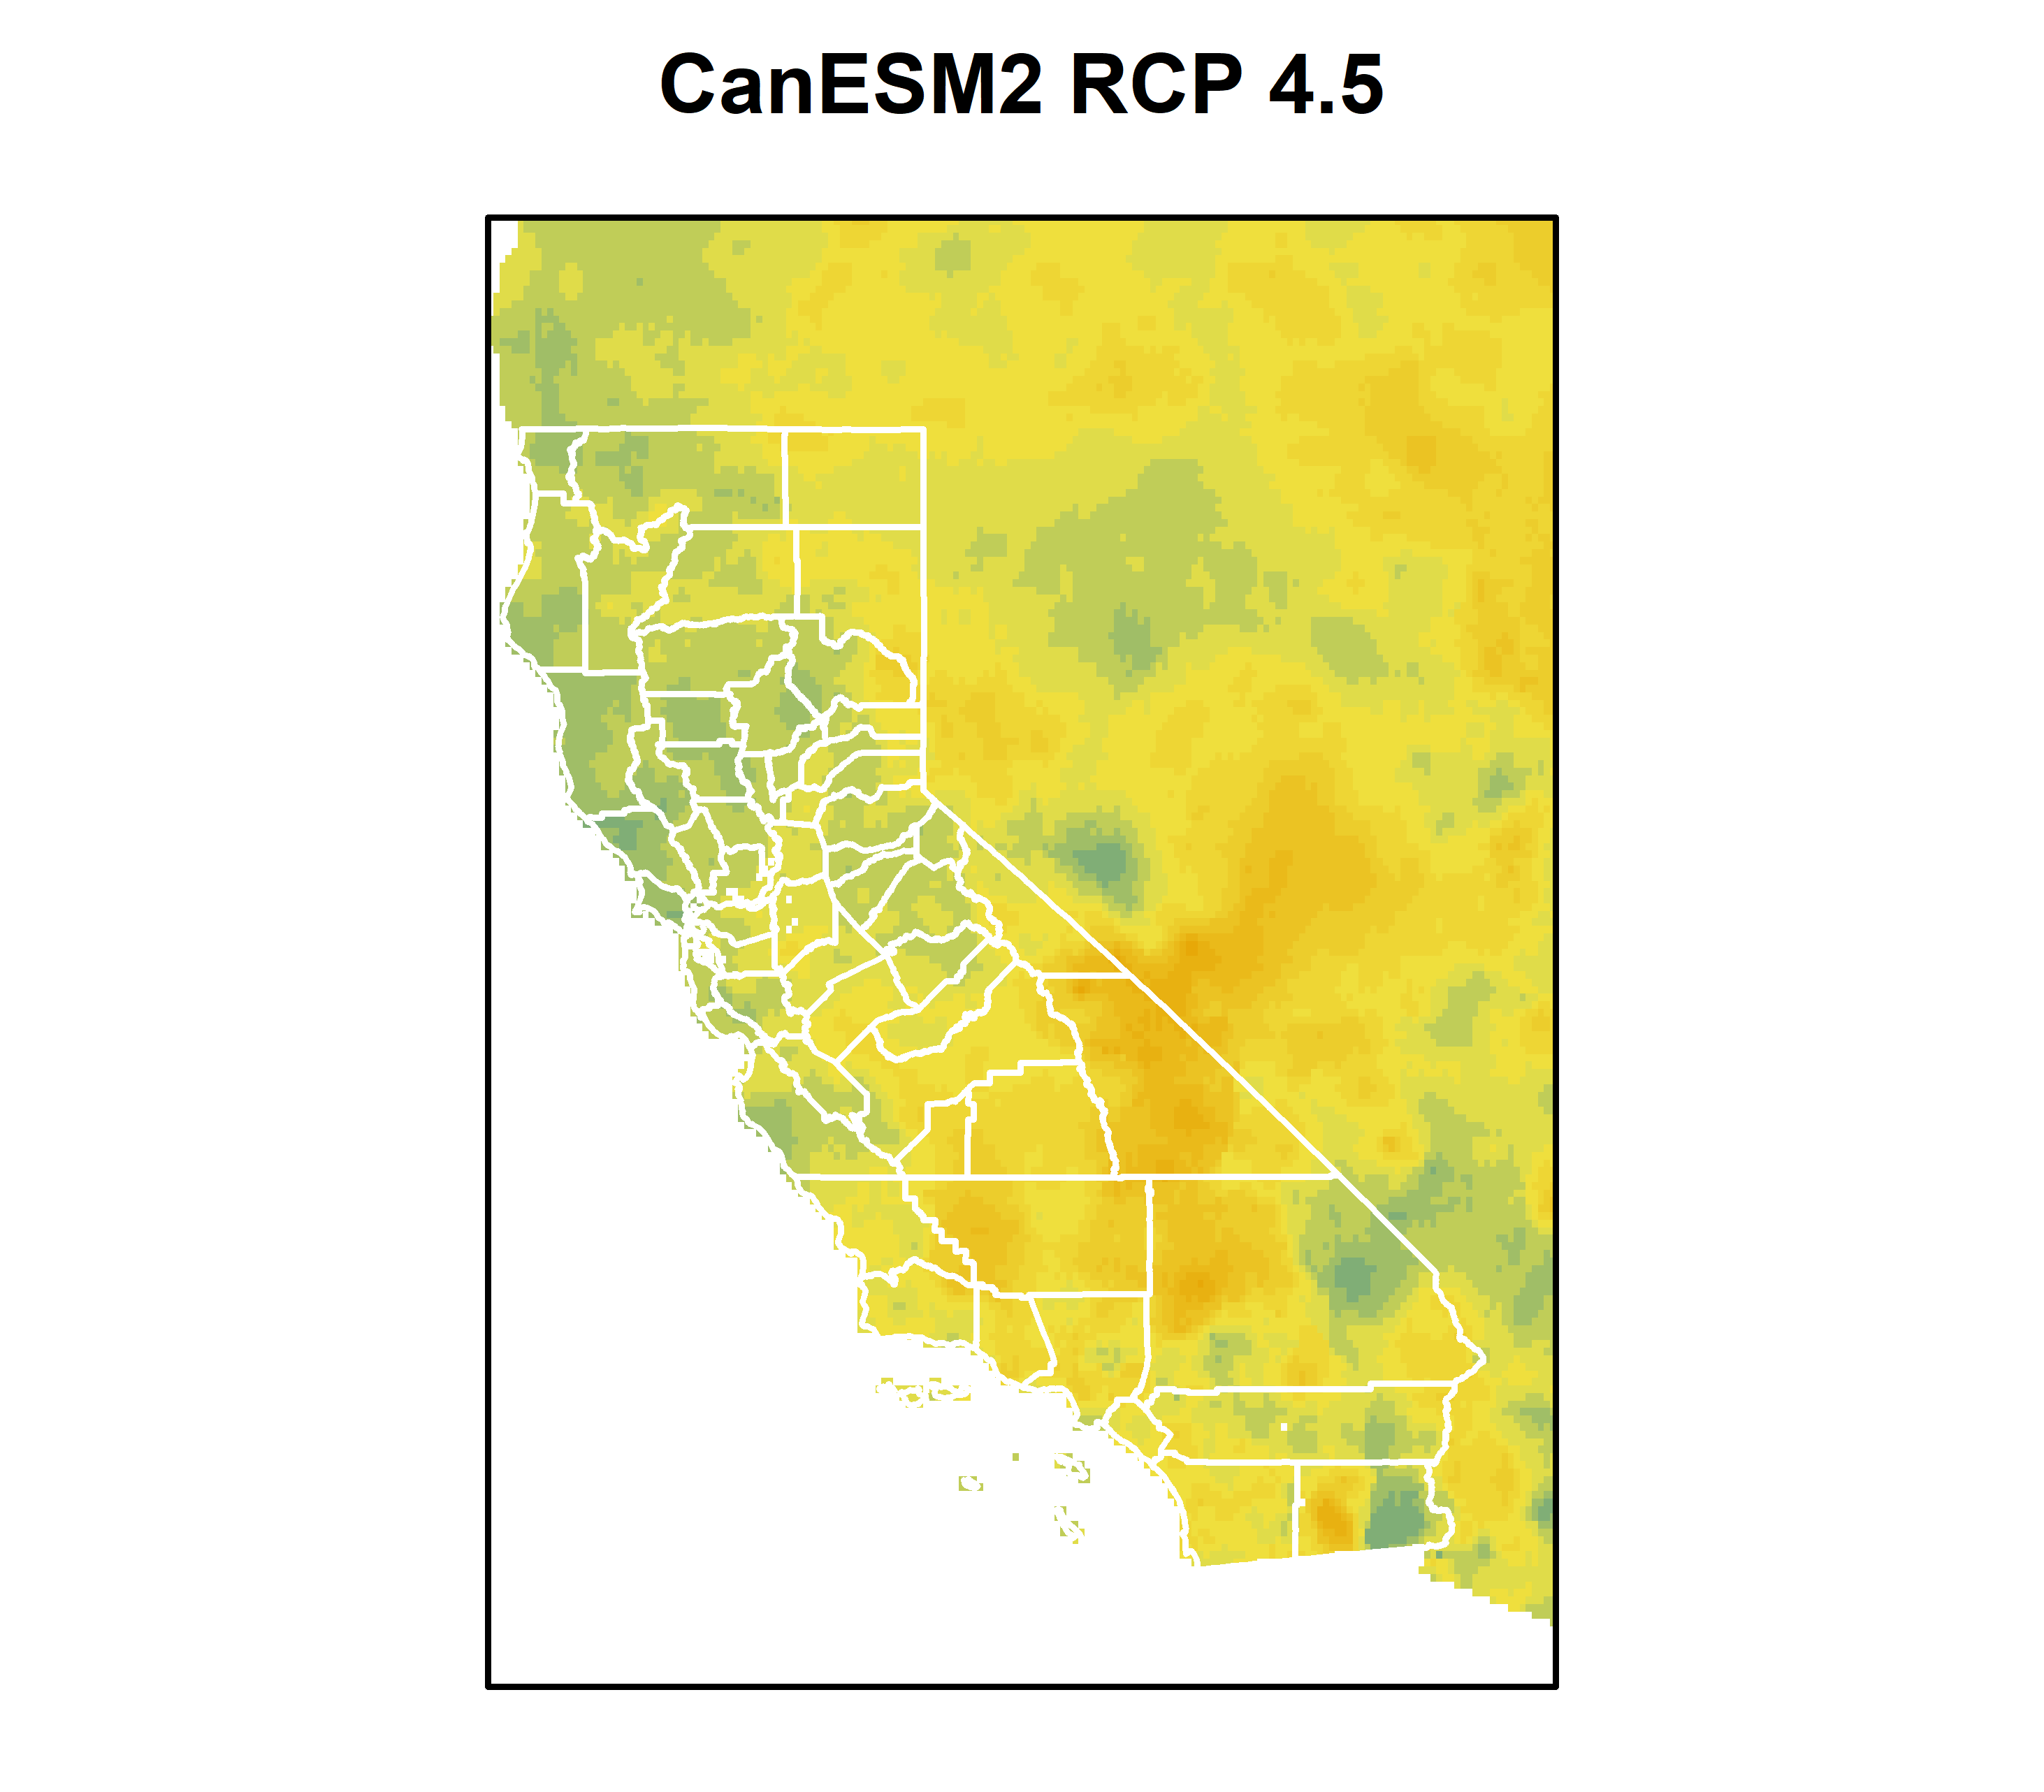
\includegraphics[width=.24\textwidth, trim={1cm 0 0 0}]{plots/rplot54_PPT_CanESM2_45_rpd.png}\hfill
    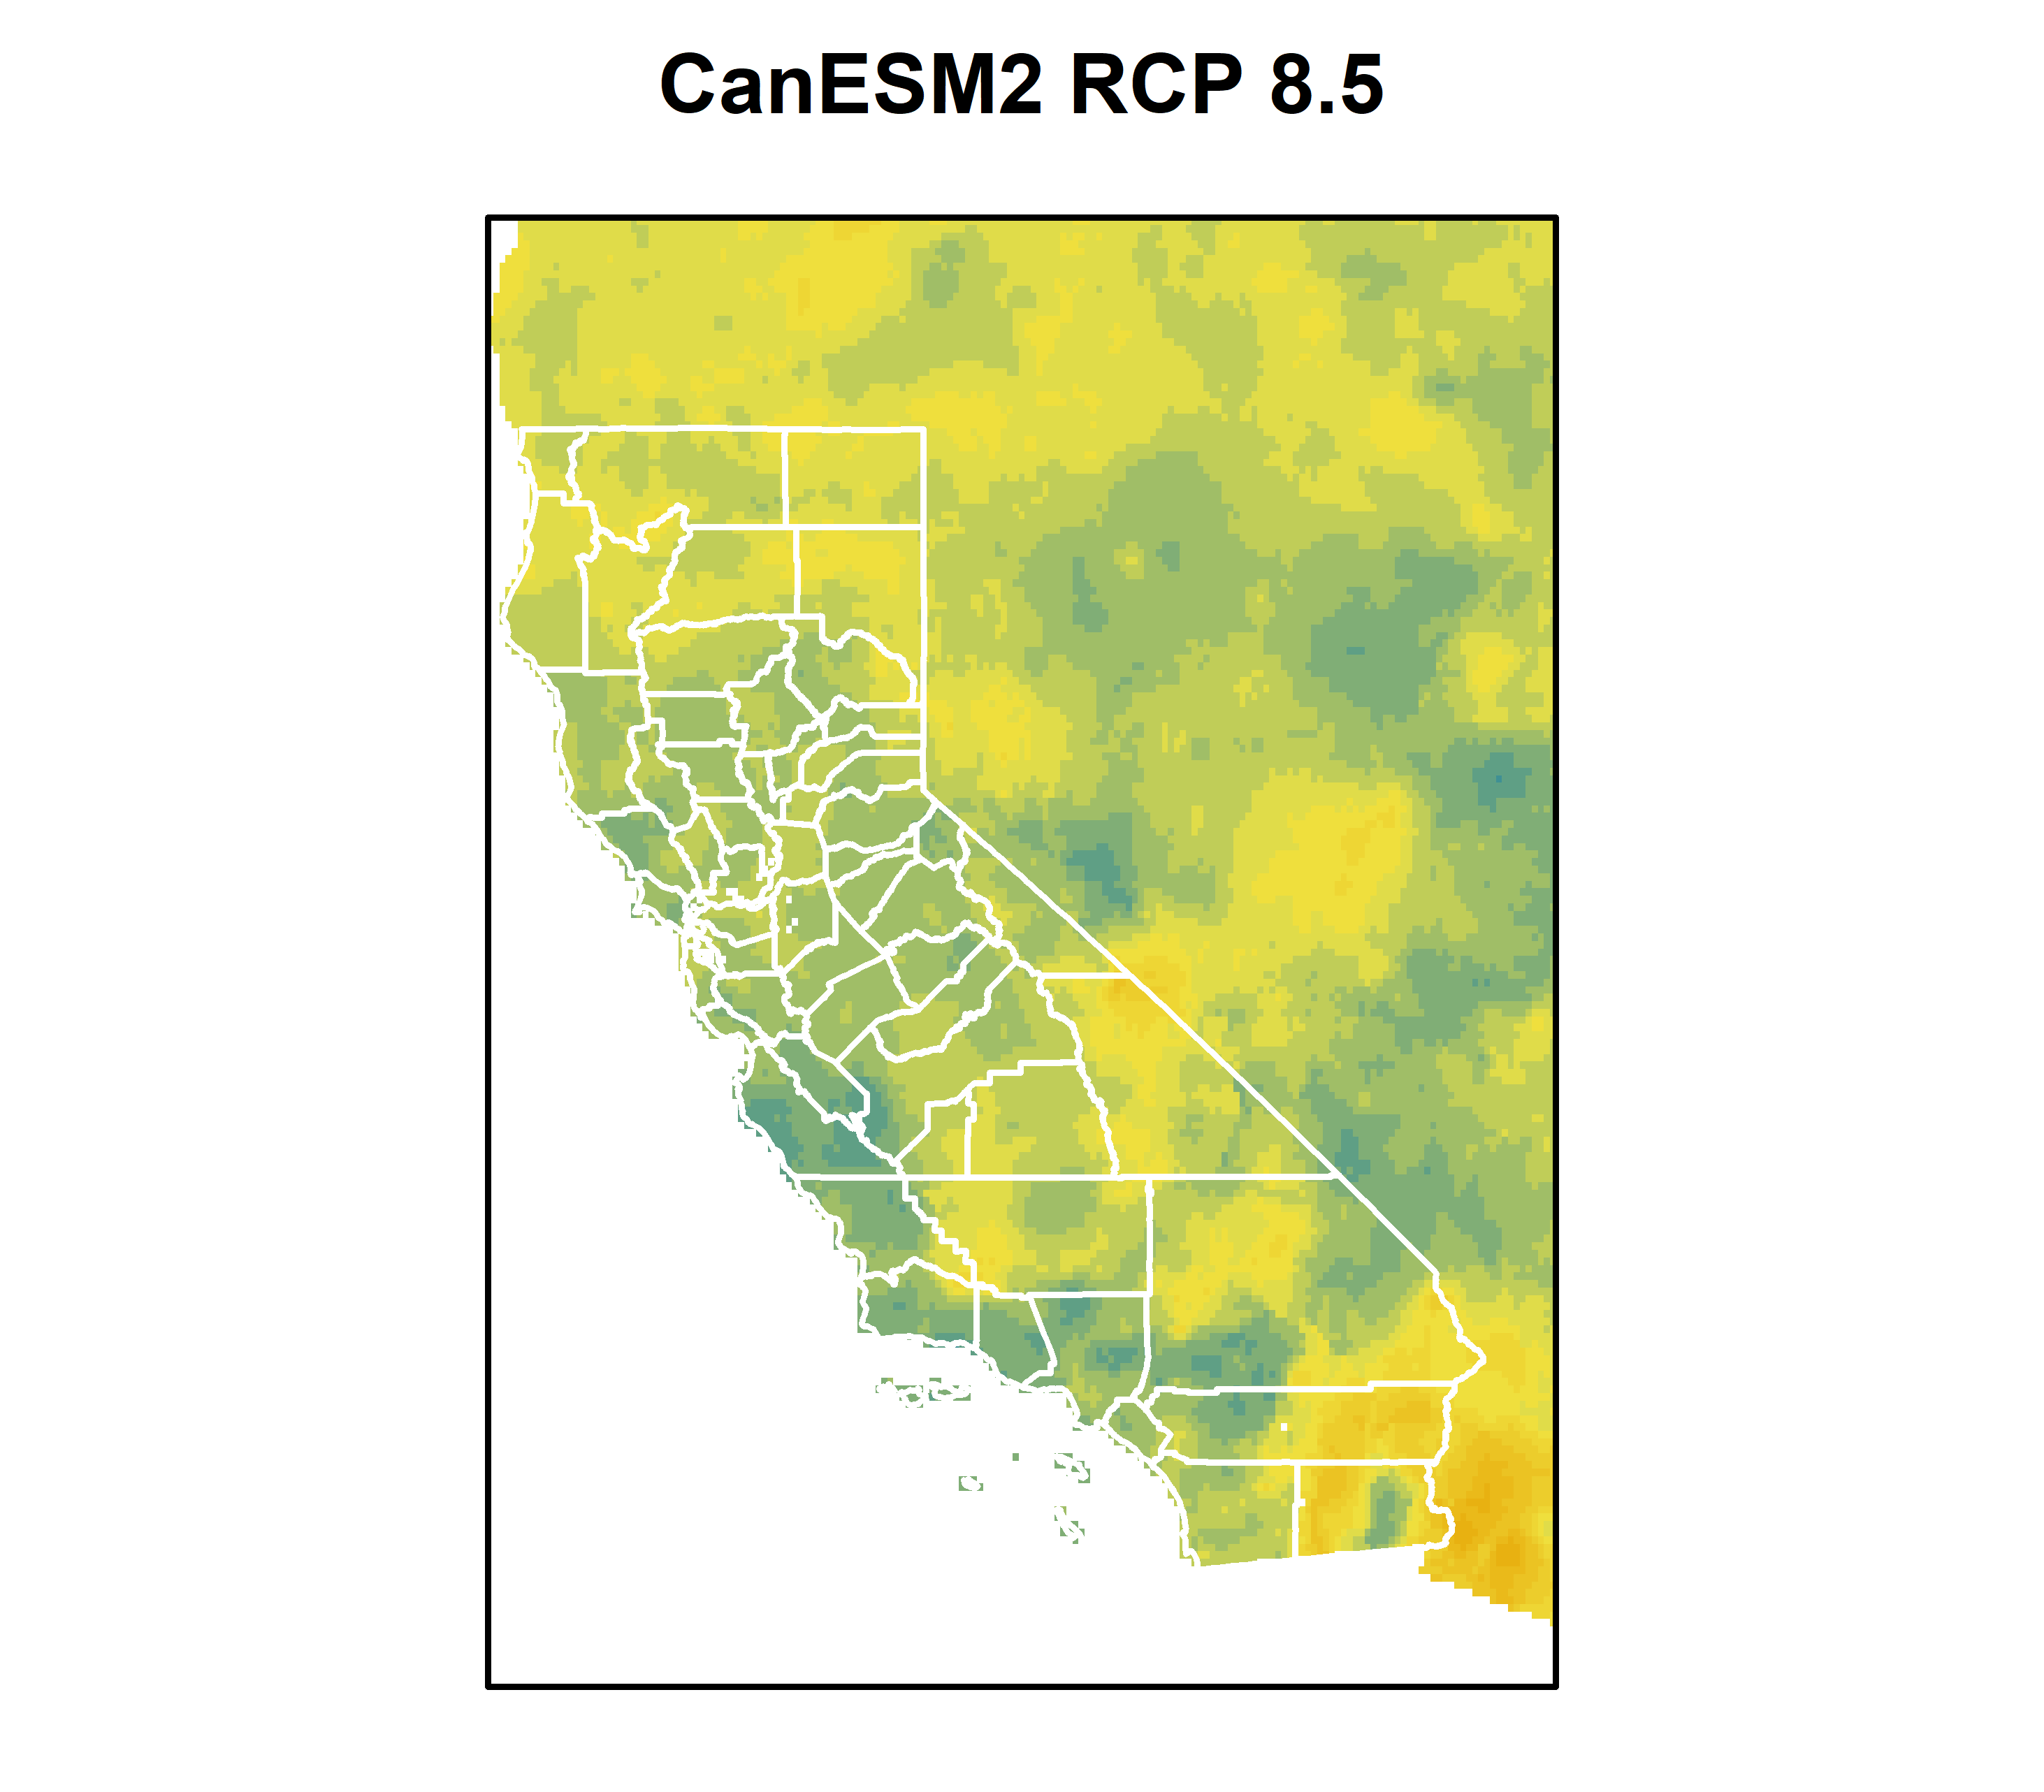
\includegraphics[width=.24\textwidth, trim={1cm 0 0 0}]{plots/rplot54_PPT_CanESM2_85_rpd.png}\hfill
    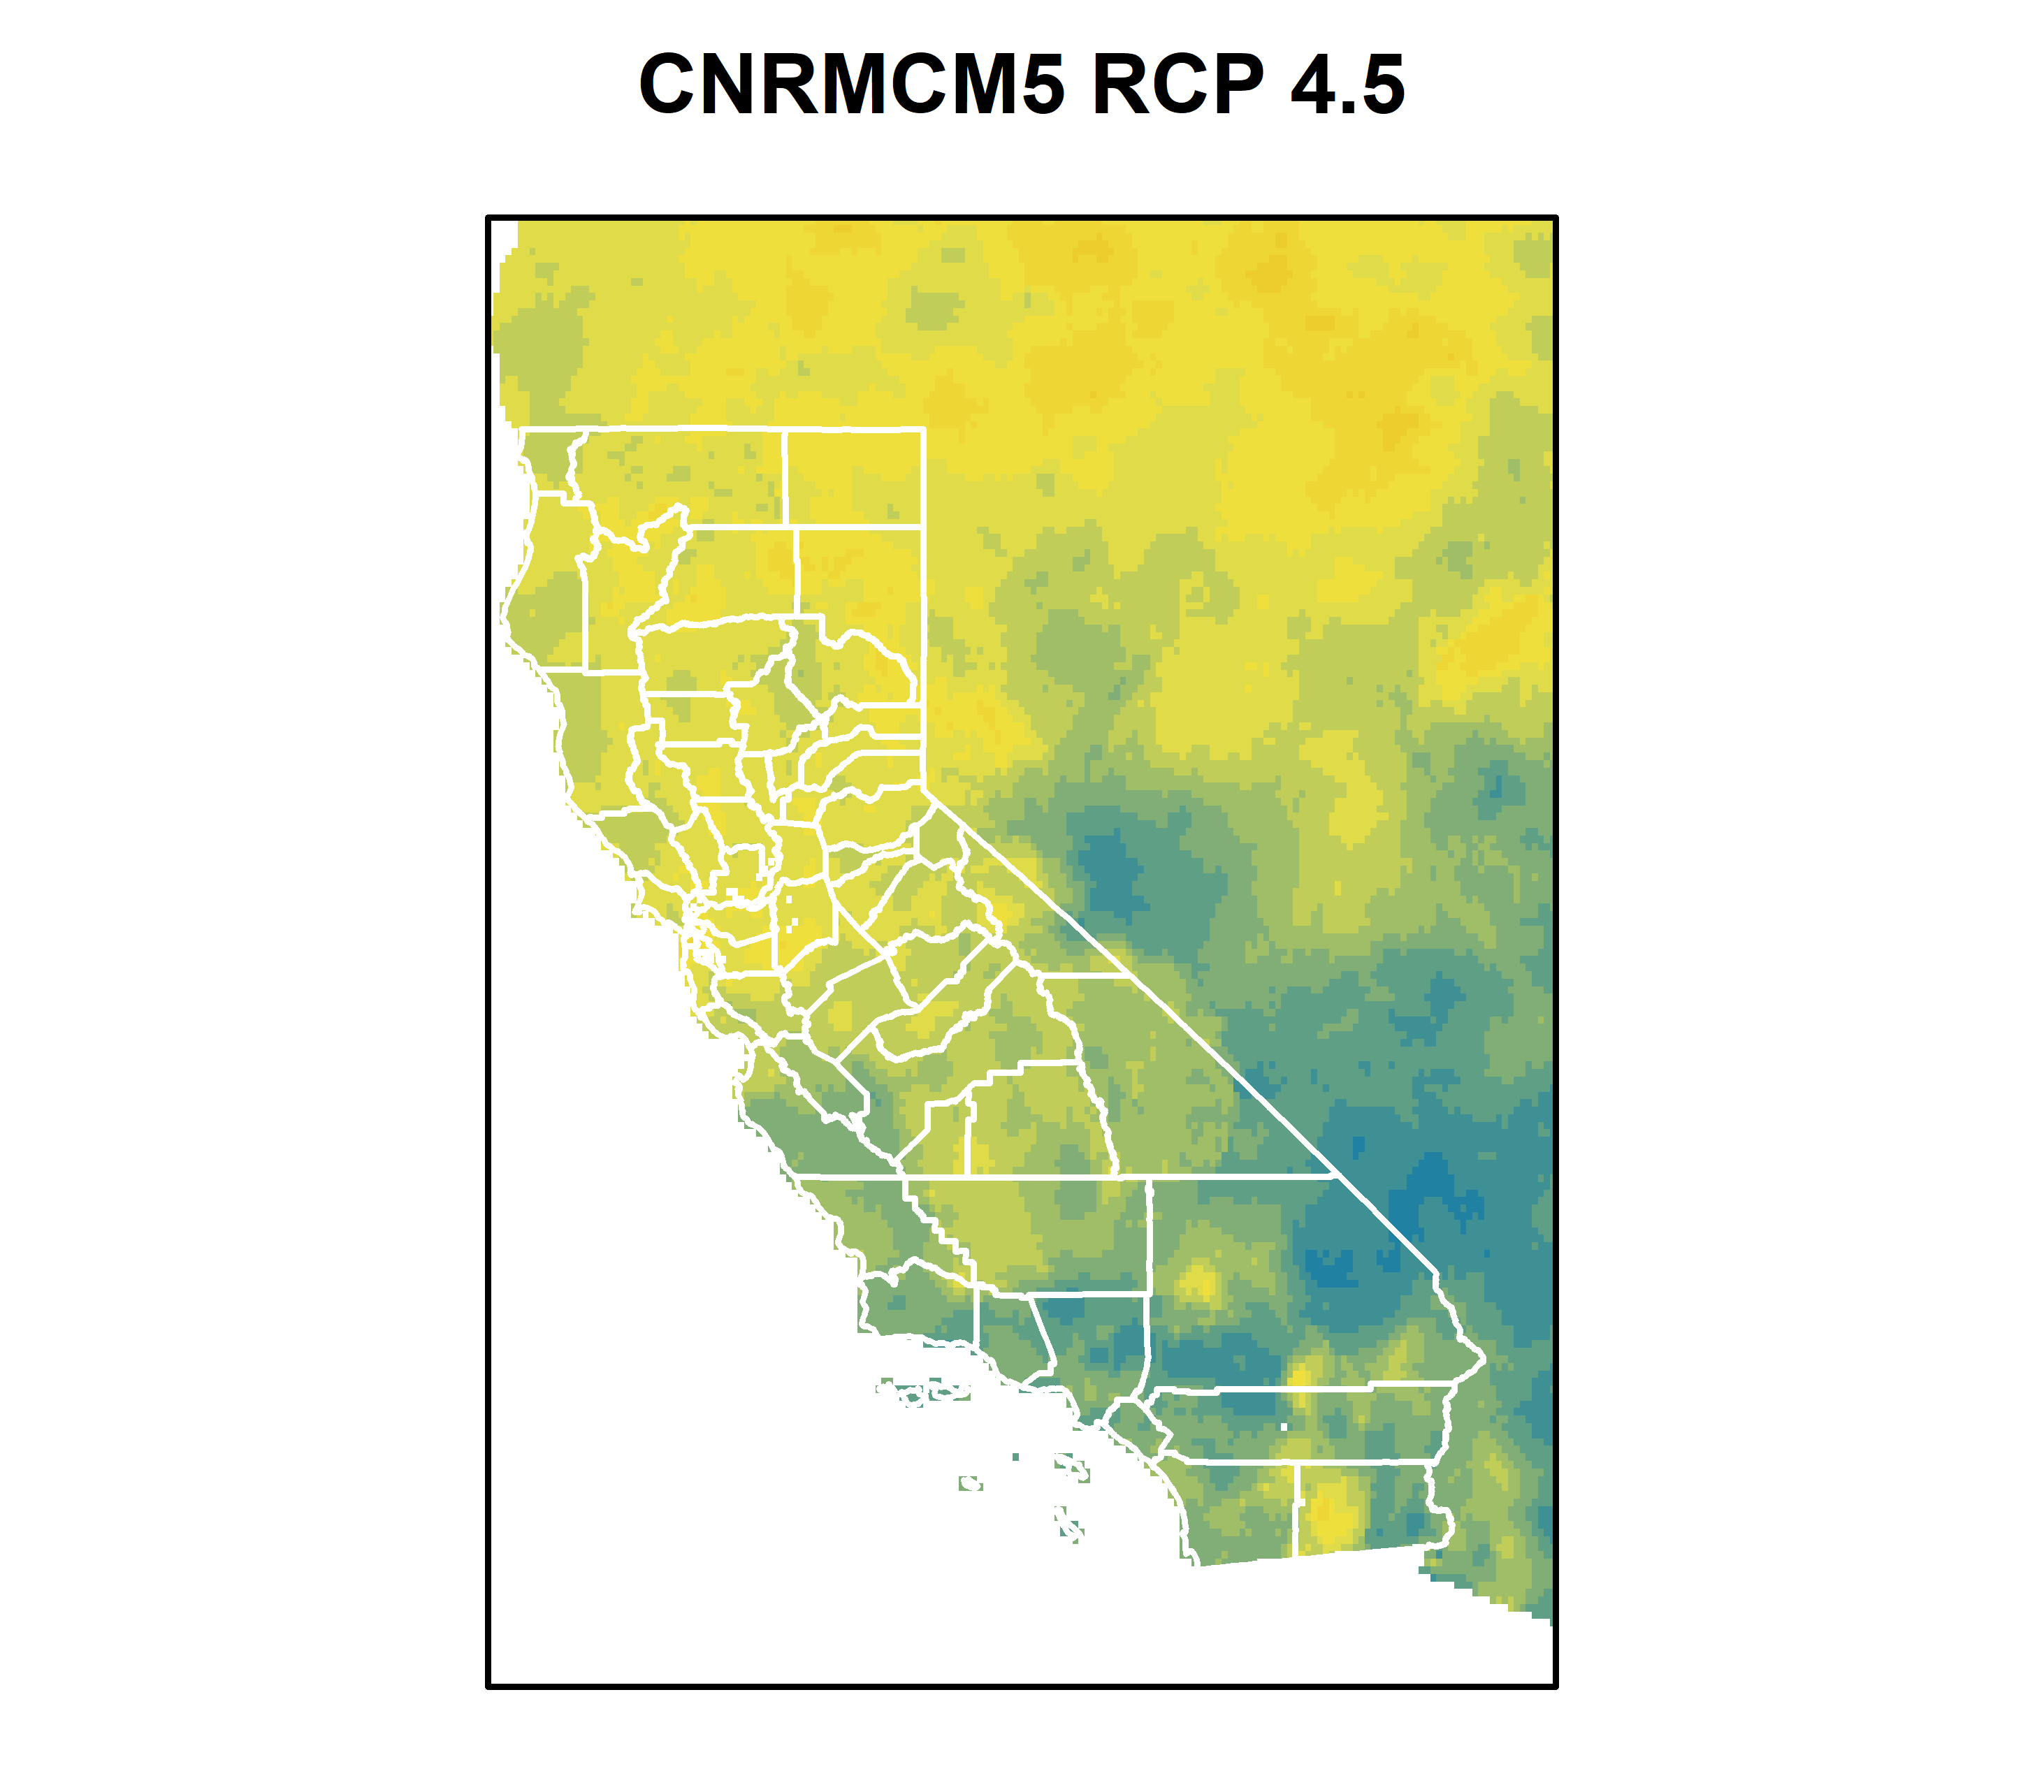
\includegraphics[width=.24\textwidth, trim={1cm 0 0 0}]{plots/rplot54_PPT_CNRMCM5_45_rpd.png}\hfill
    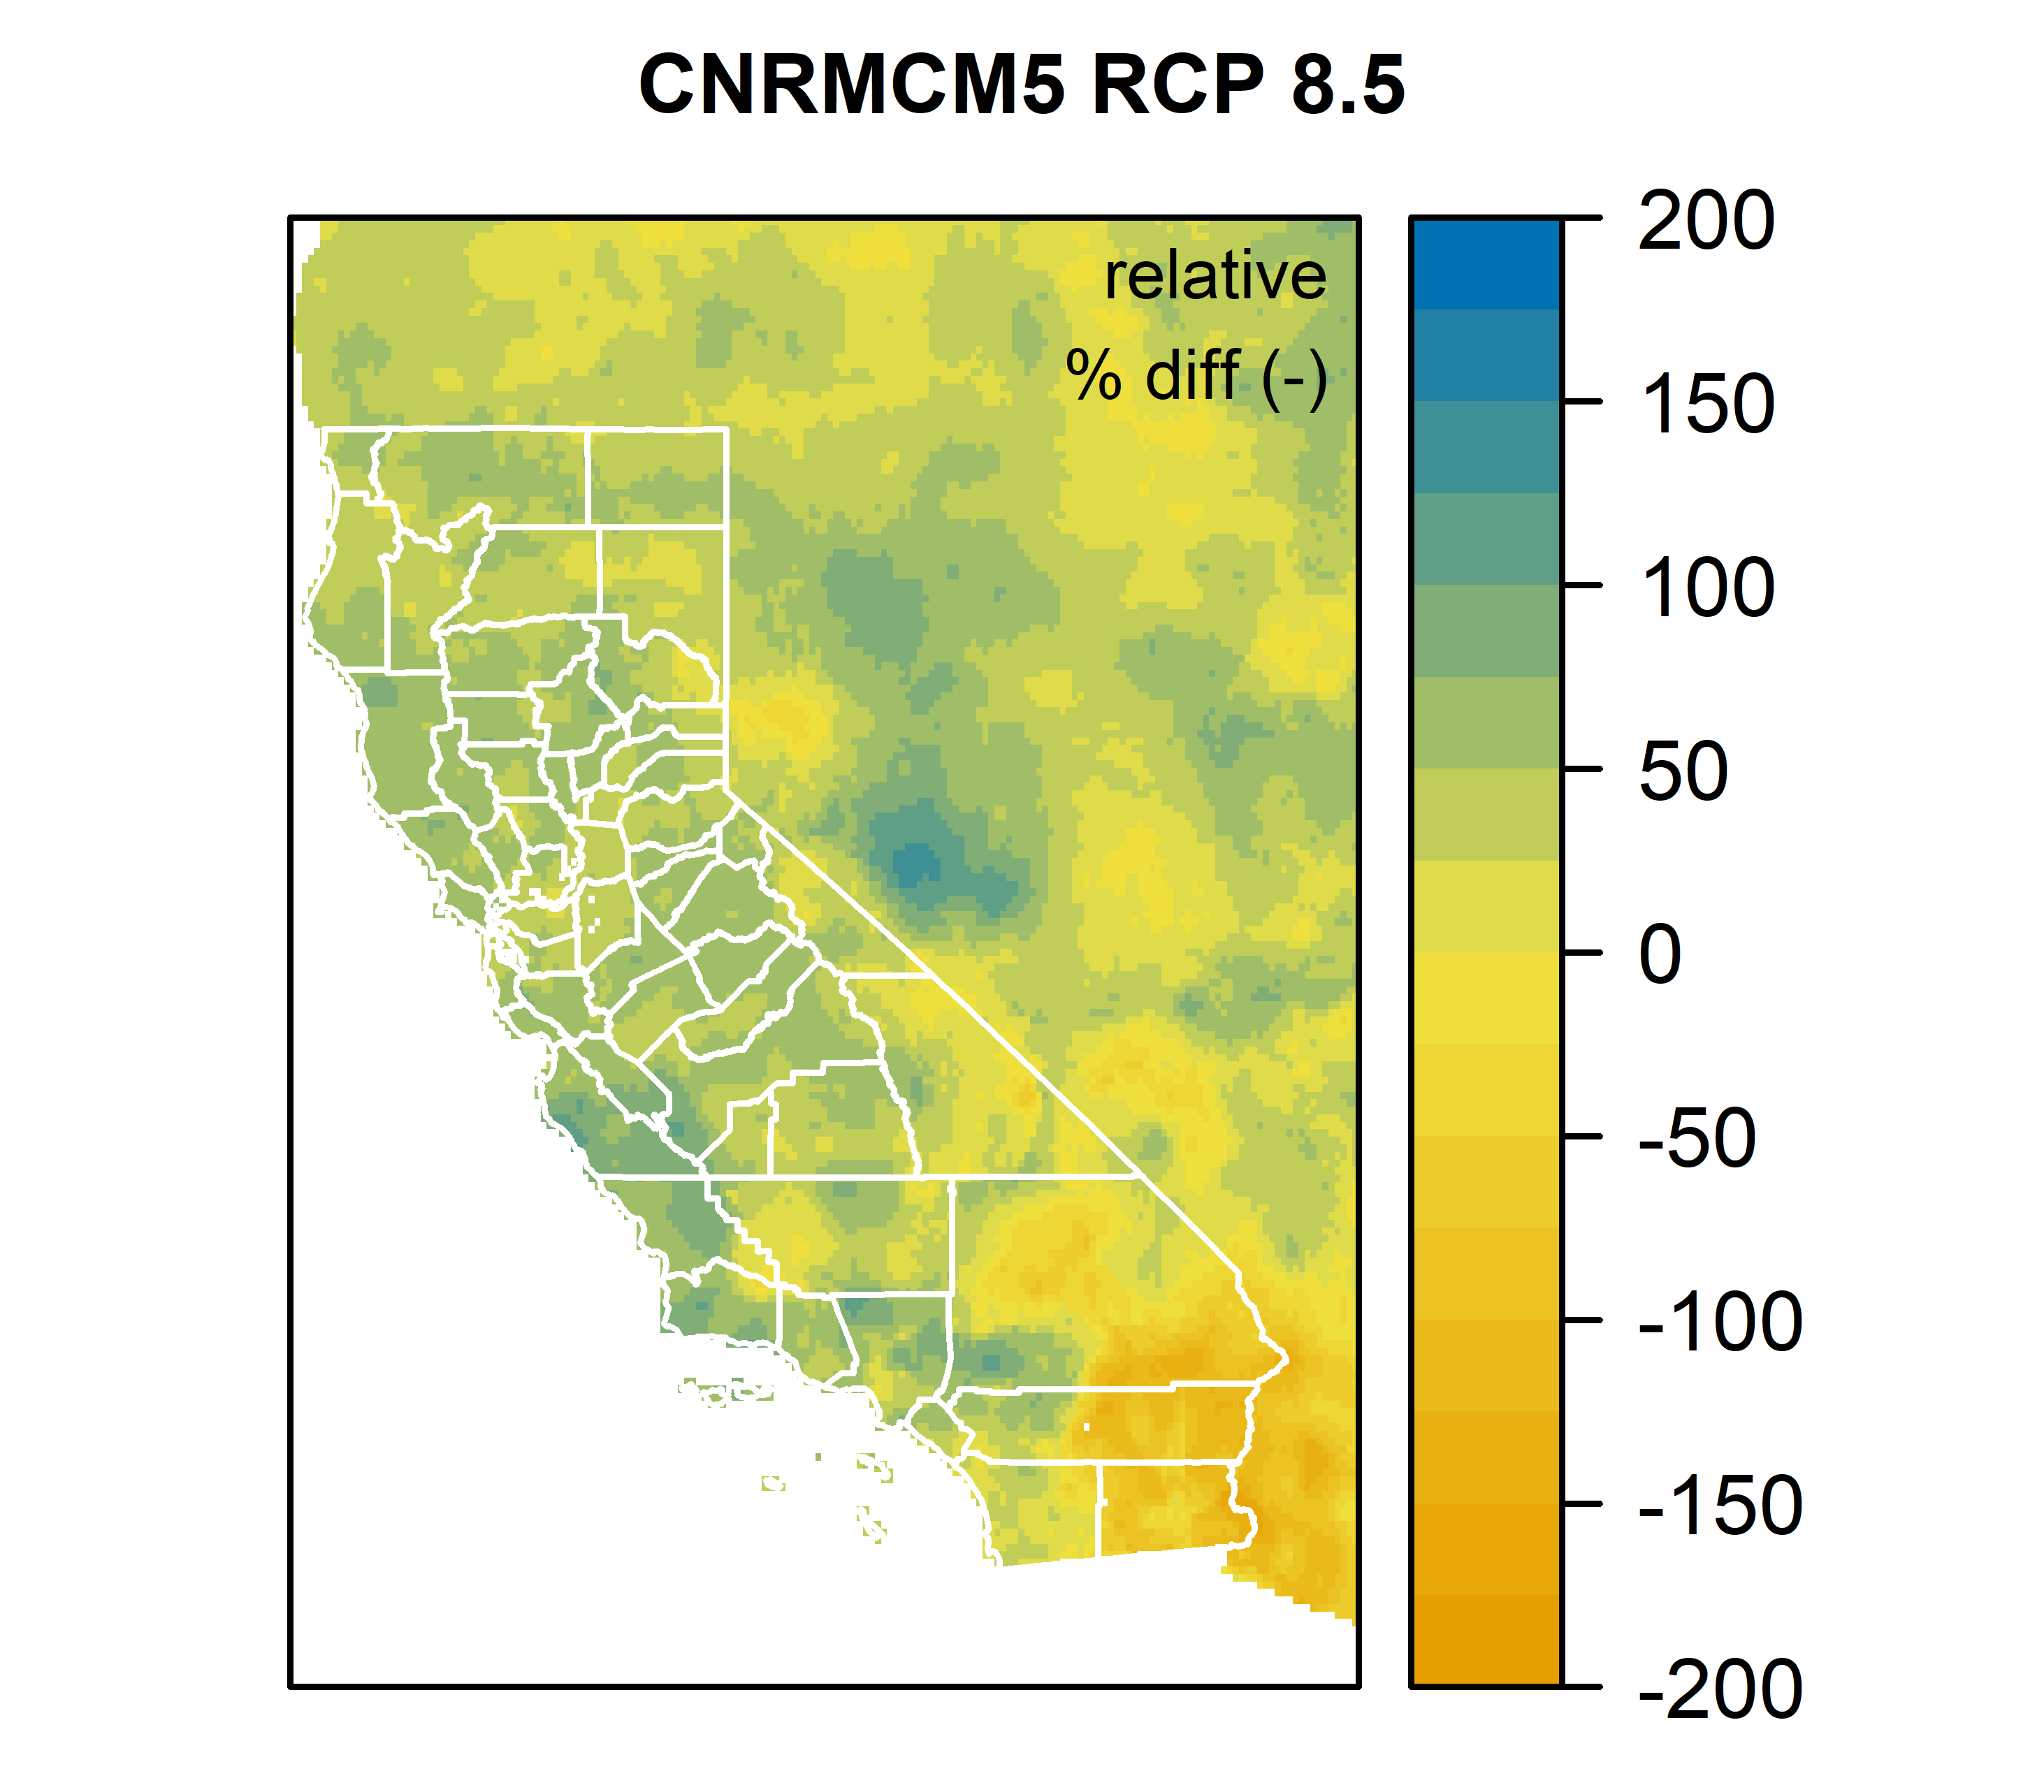
\includegraphics[width=.24\textwidth, trim={1cm 0 0 0}]{plots/rplot54_PPT_CNRMCM5_85_rpd.png}
    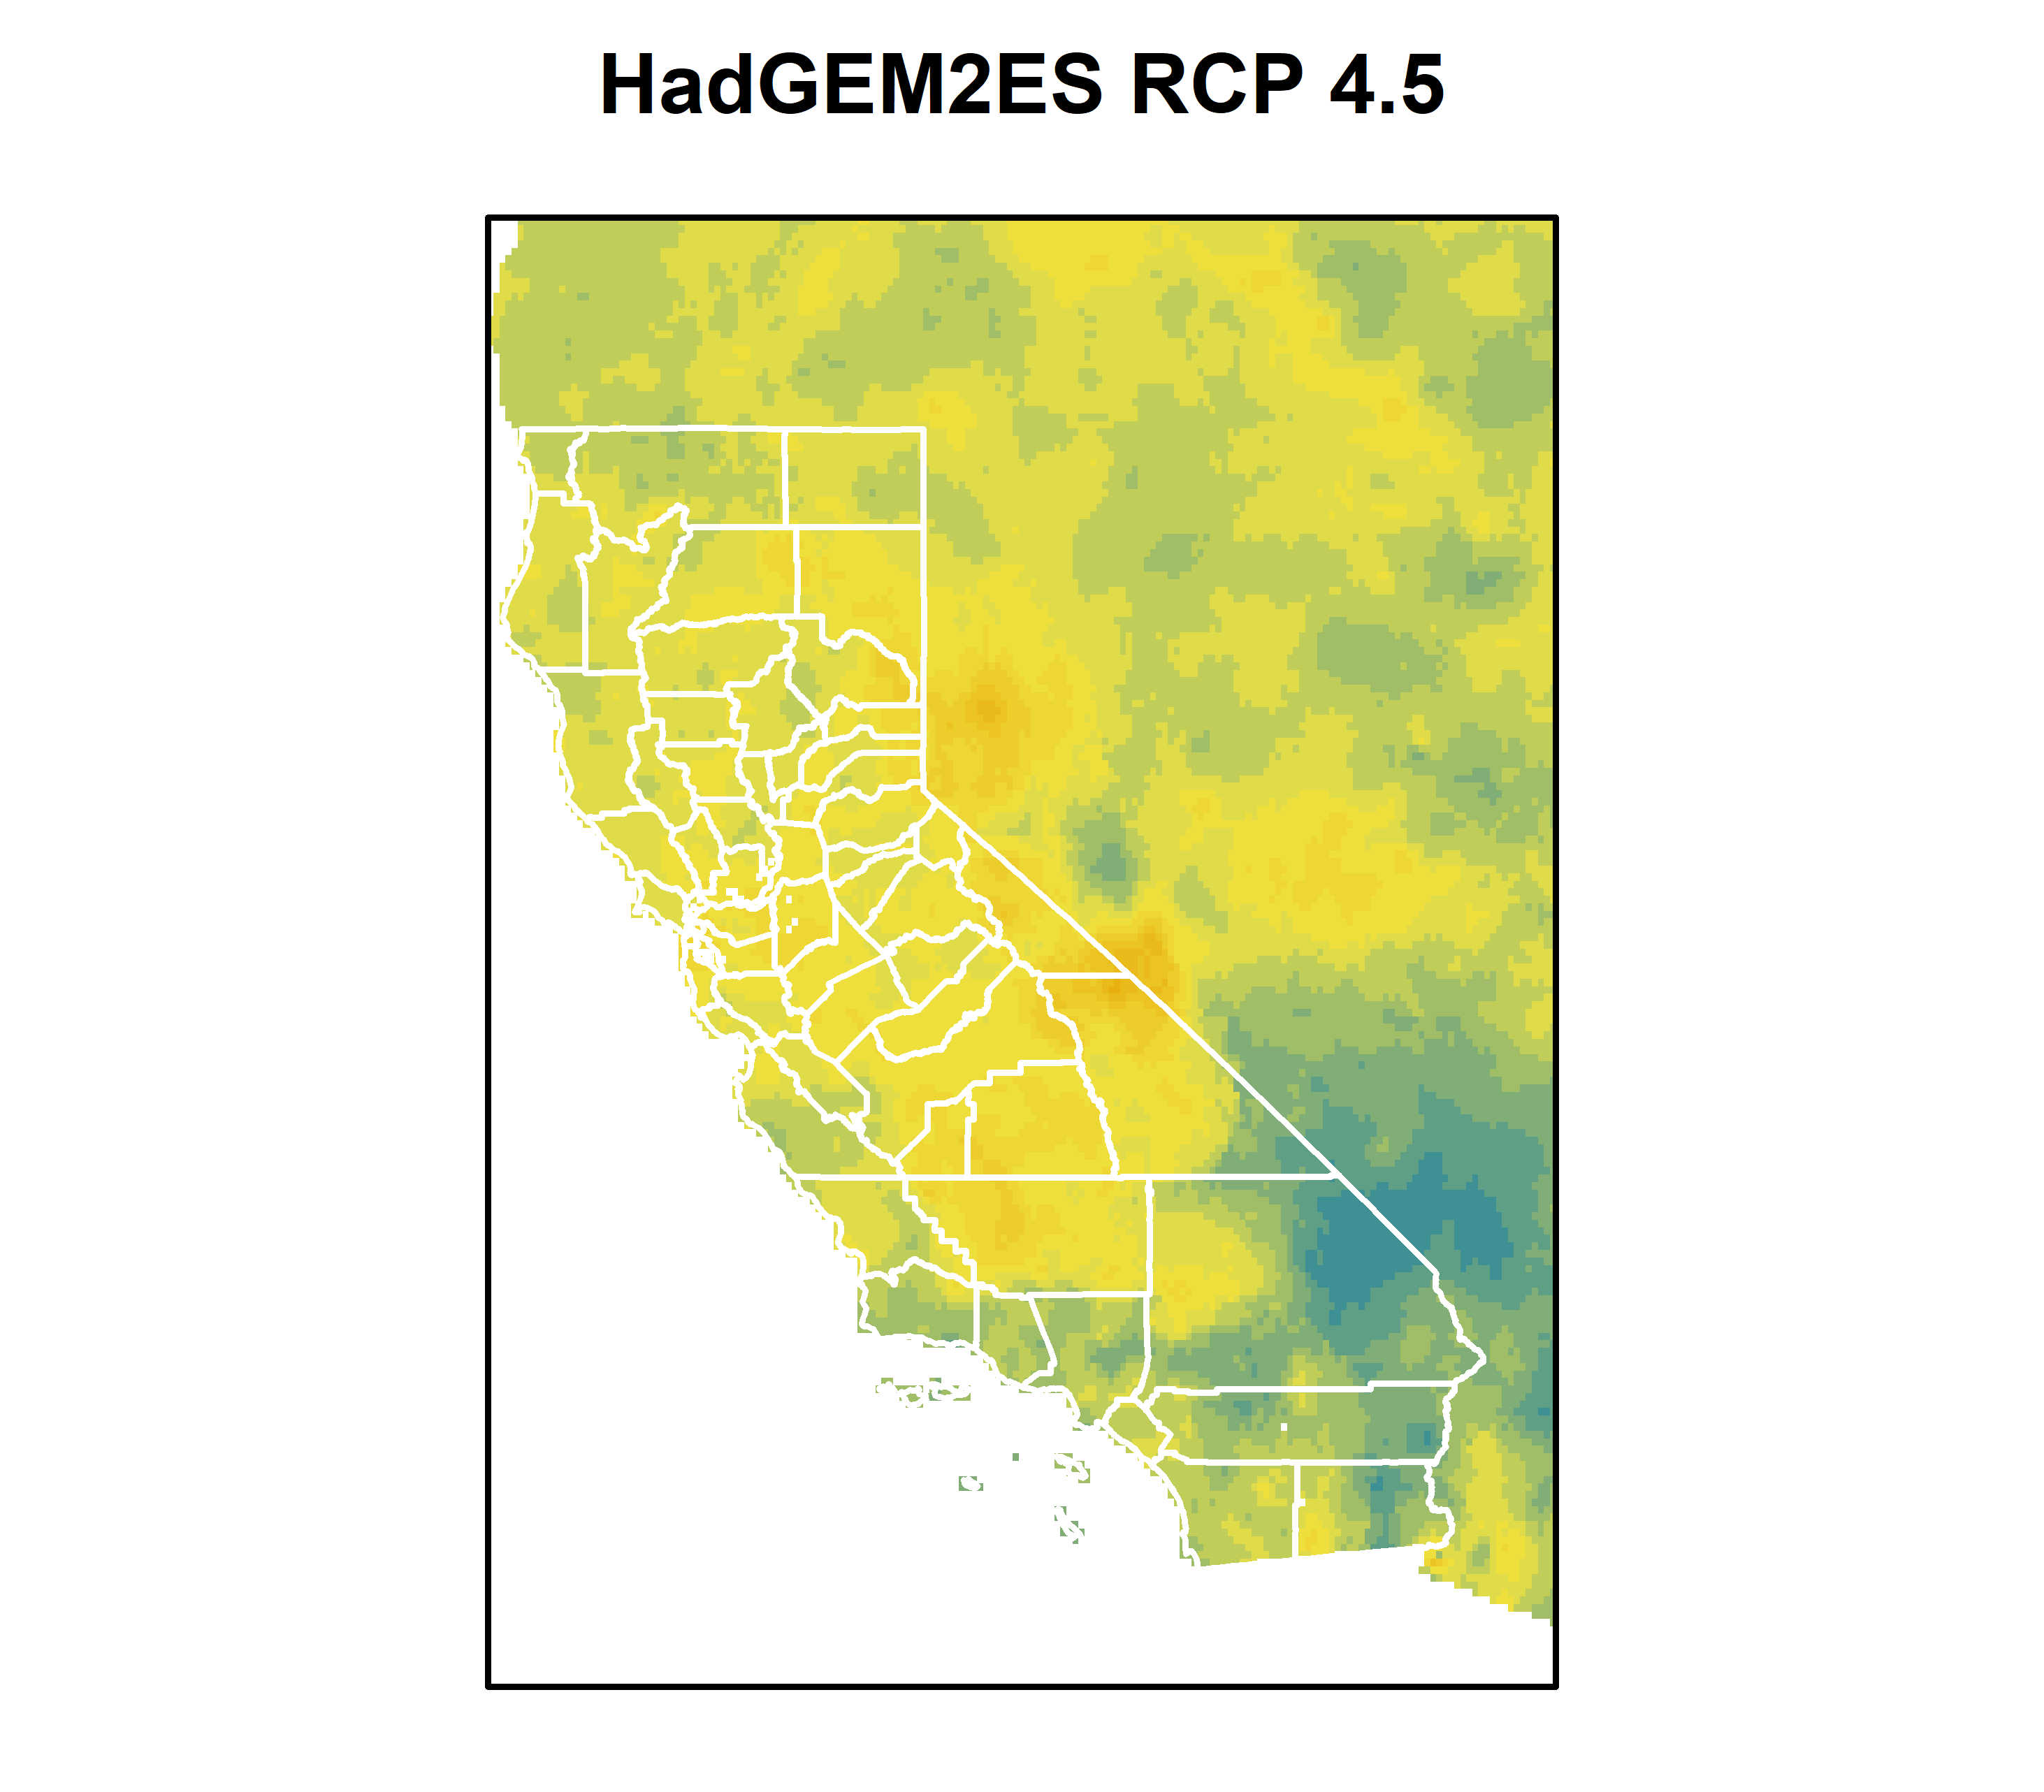
\includegraphics[width=.24\textwidth, trim={1cm 0 0 0}]{plots/rplot54_PPT_HadGEM2ES_45_rpd.png}\hfill
    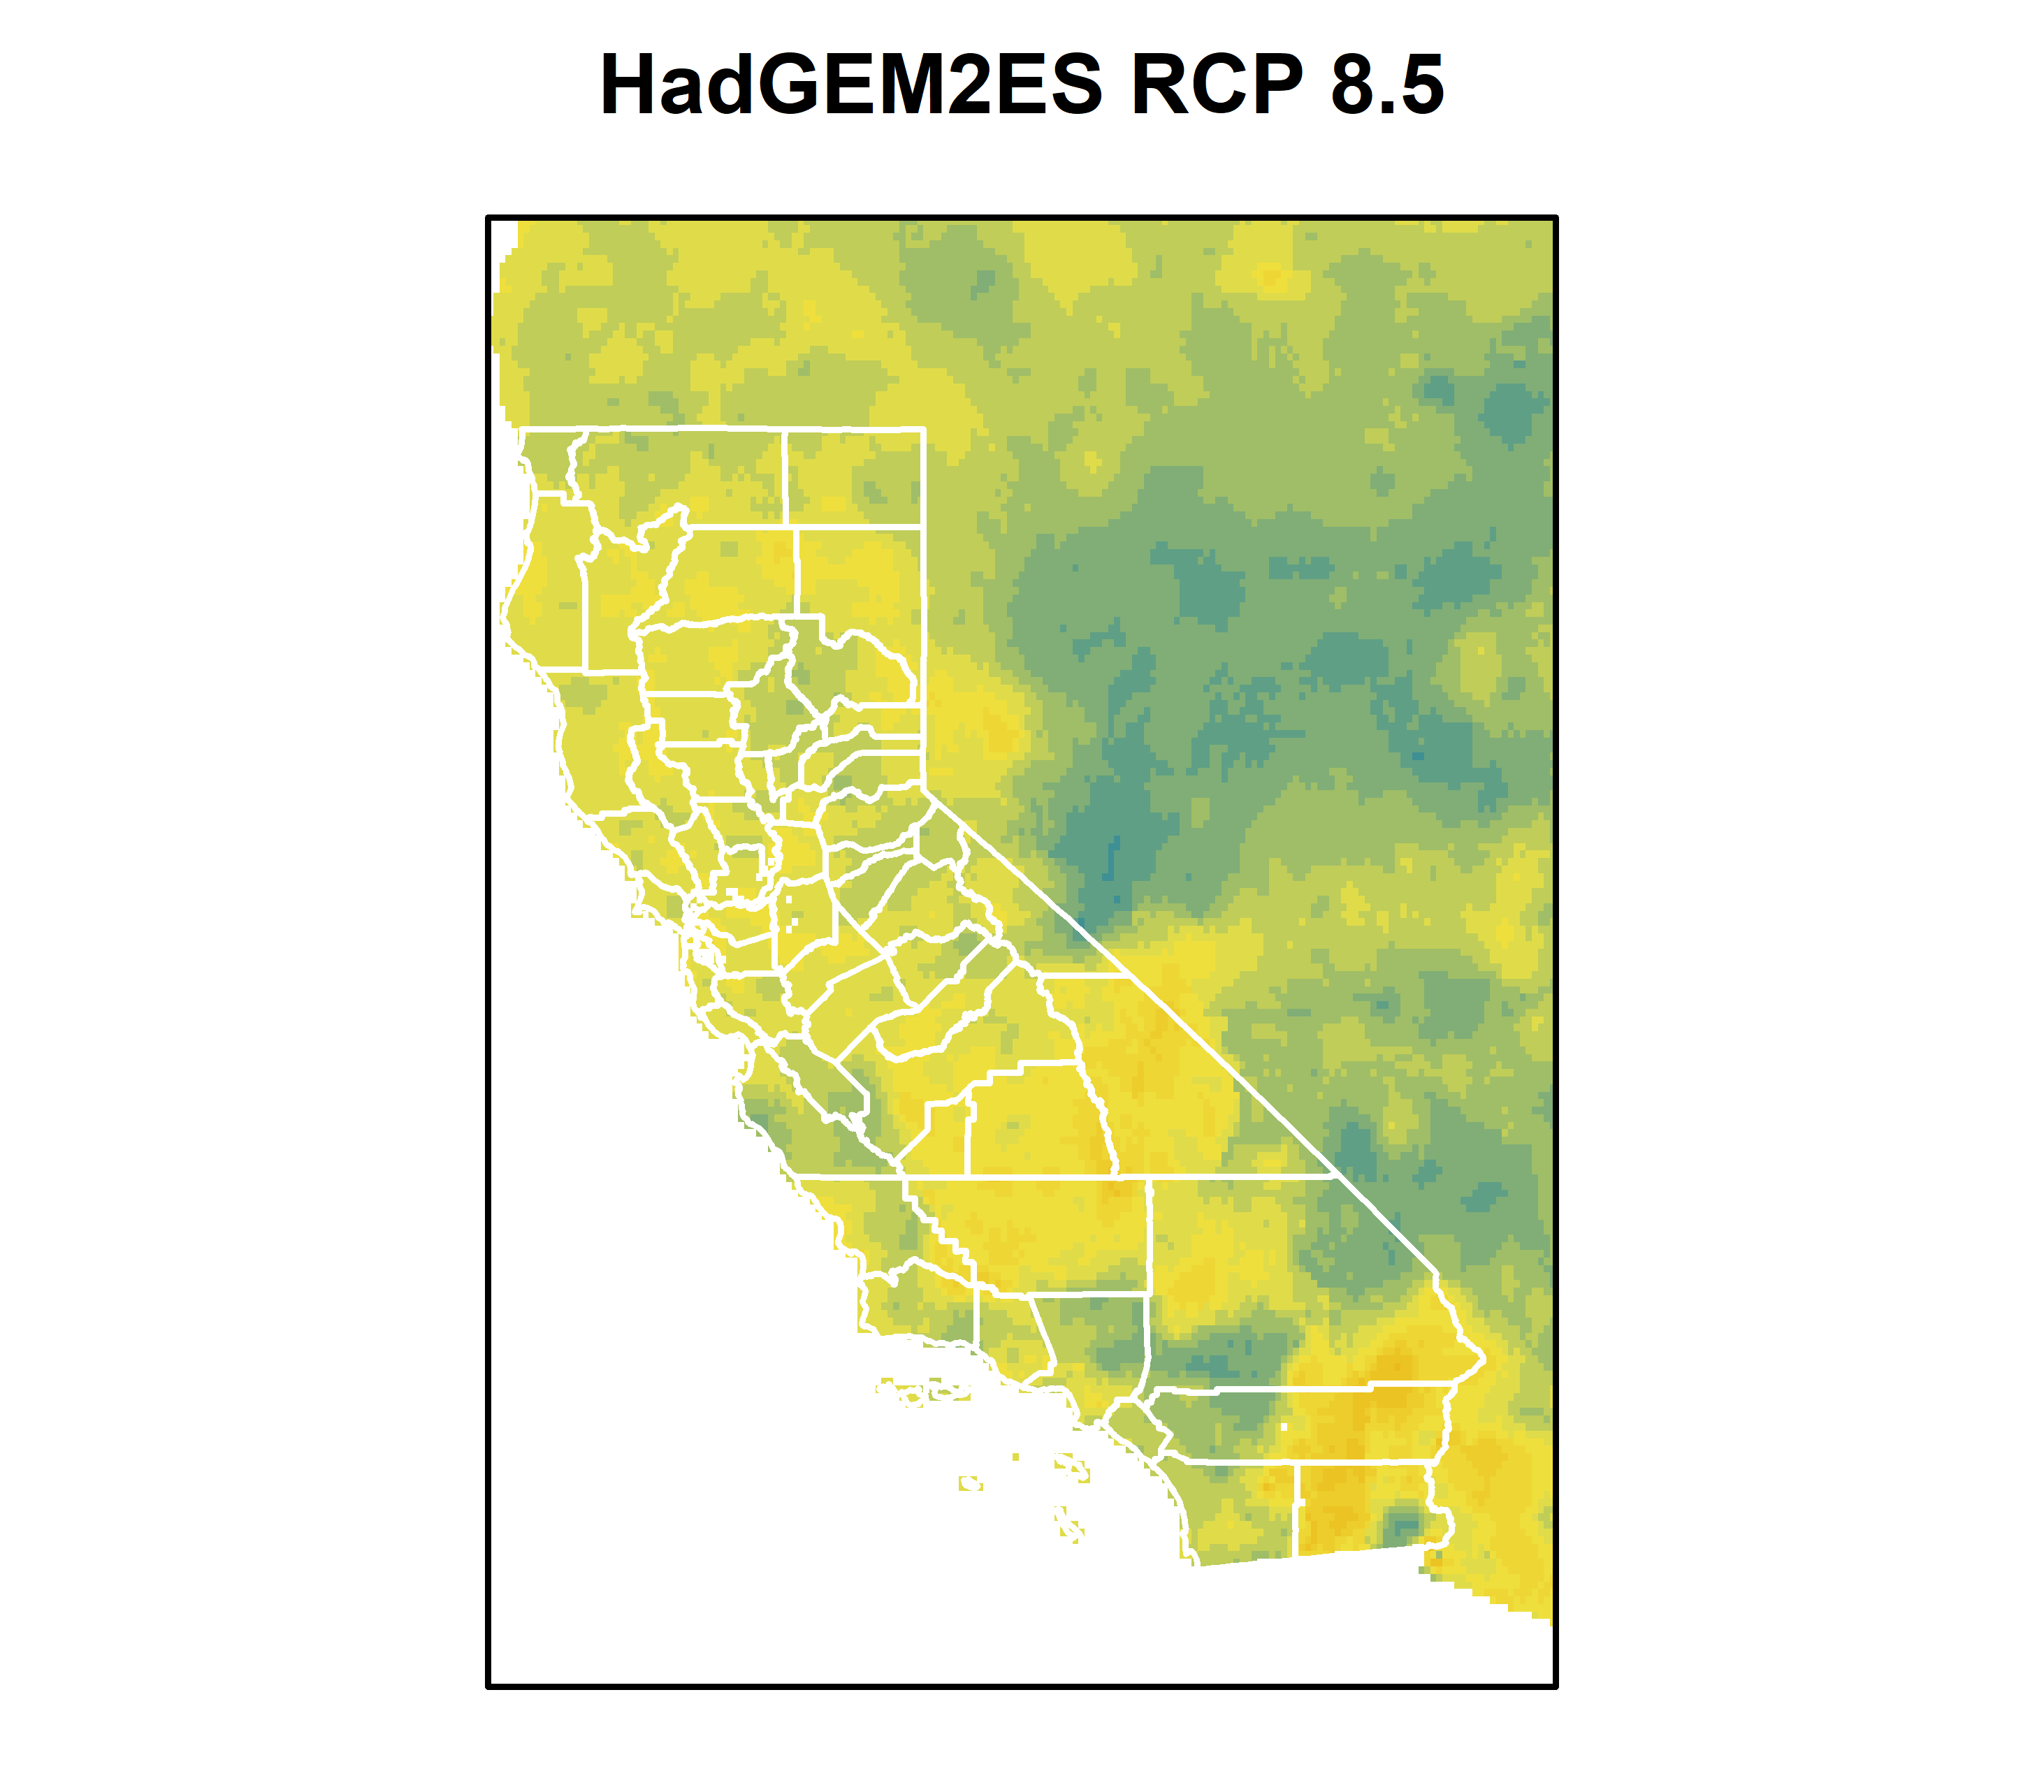
\includegraphics[width=.24\textwidth, trim={1cm 0 0 0}]{plots/rplot54_PPT_HadGEM2ES_85_rpd.png}\hfill
    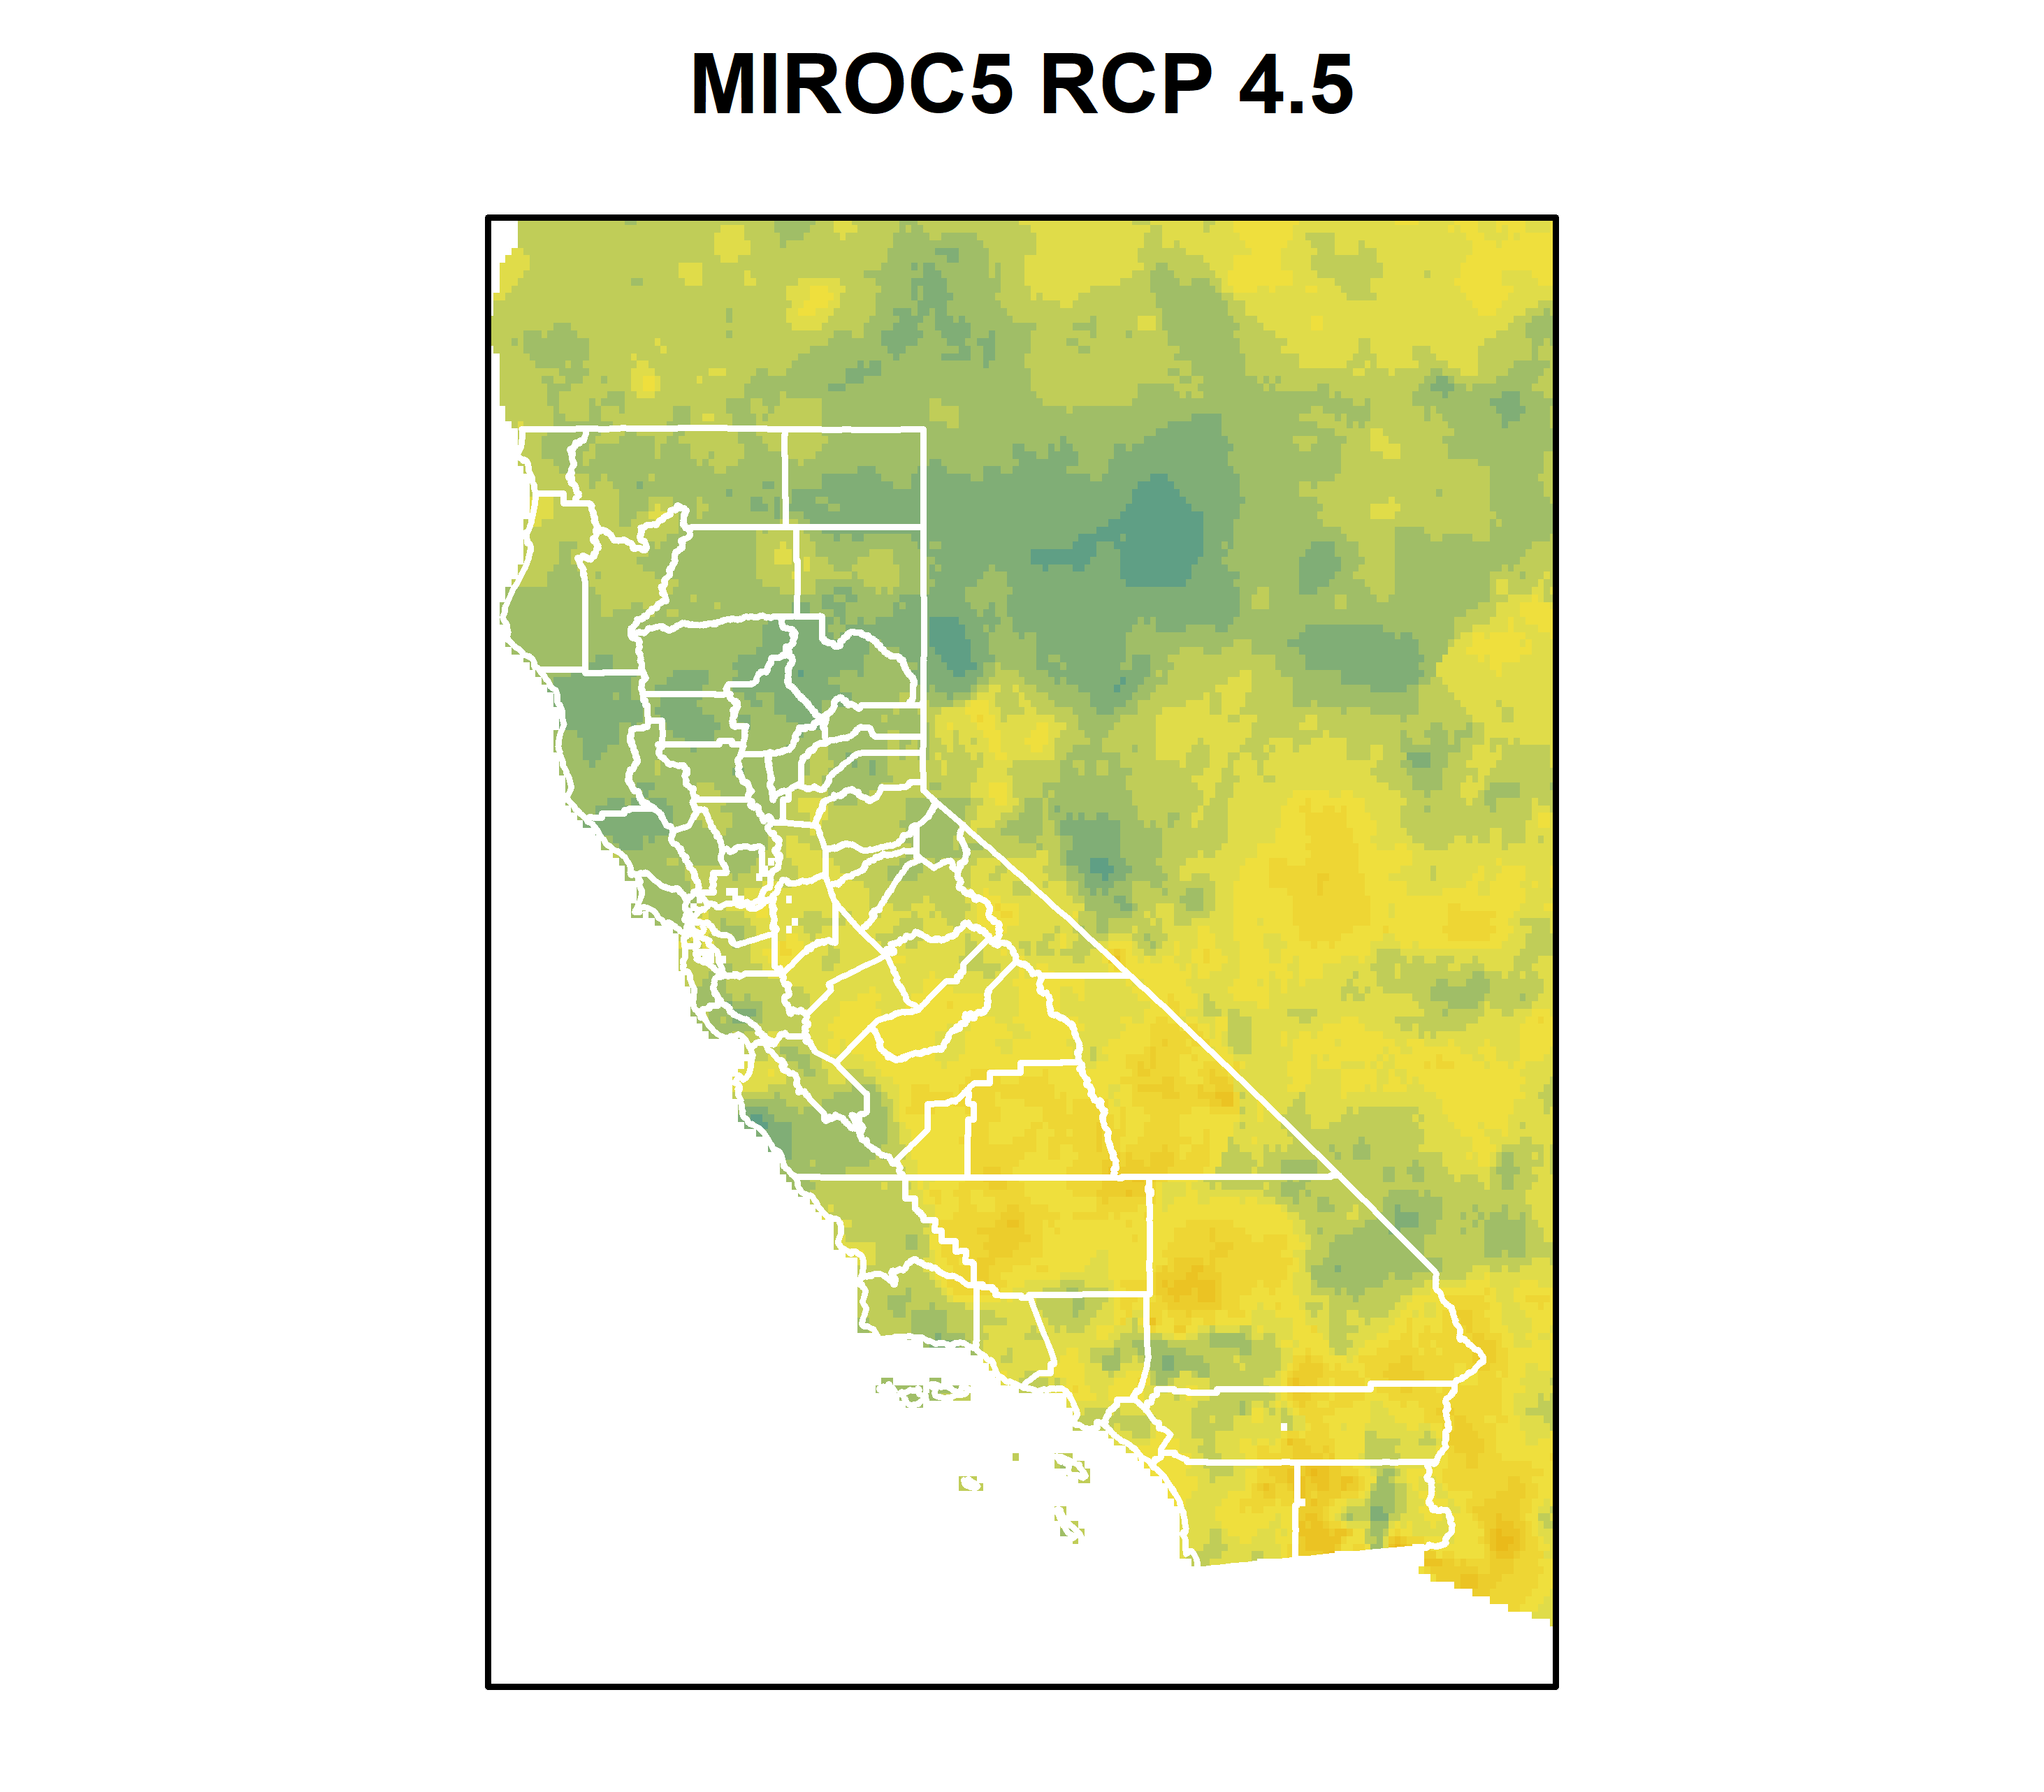
\includegraphics[width=.24\textwidth, trim={1cm 0 0 0}]{plots/rplot54_PPT_MIROC5_45_rpd.png}\hfill
    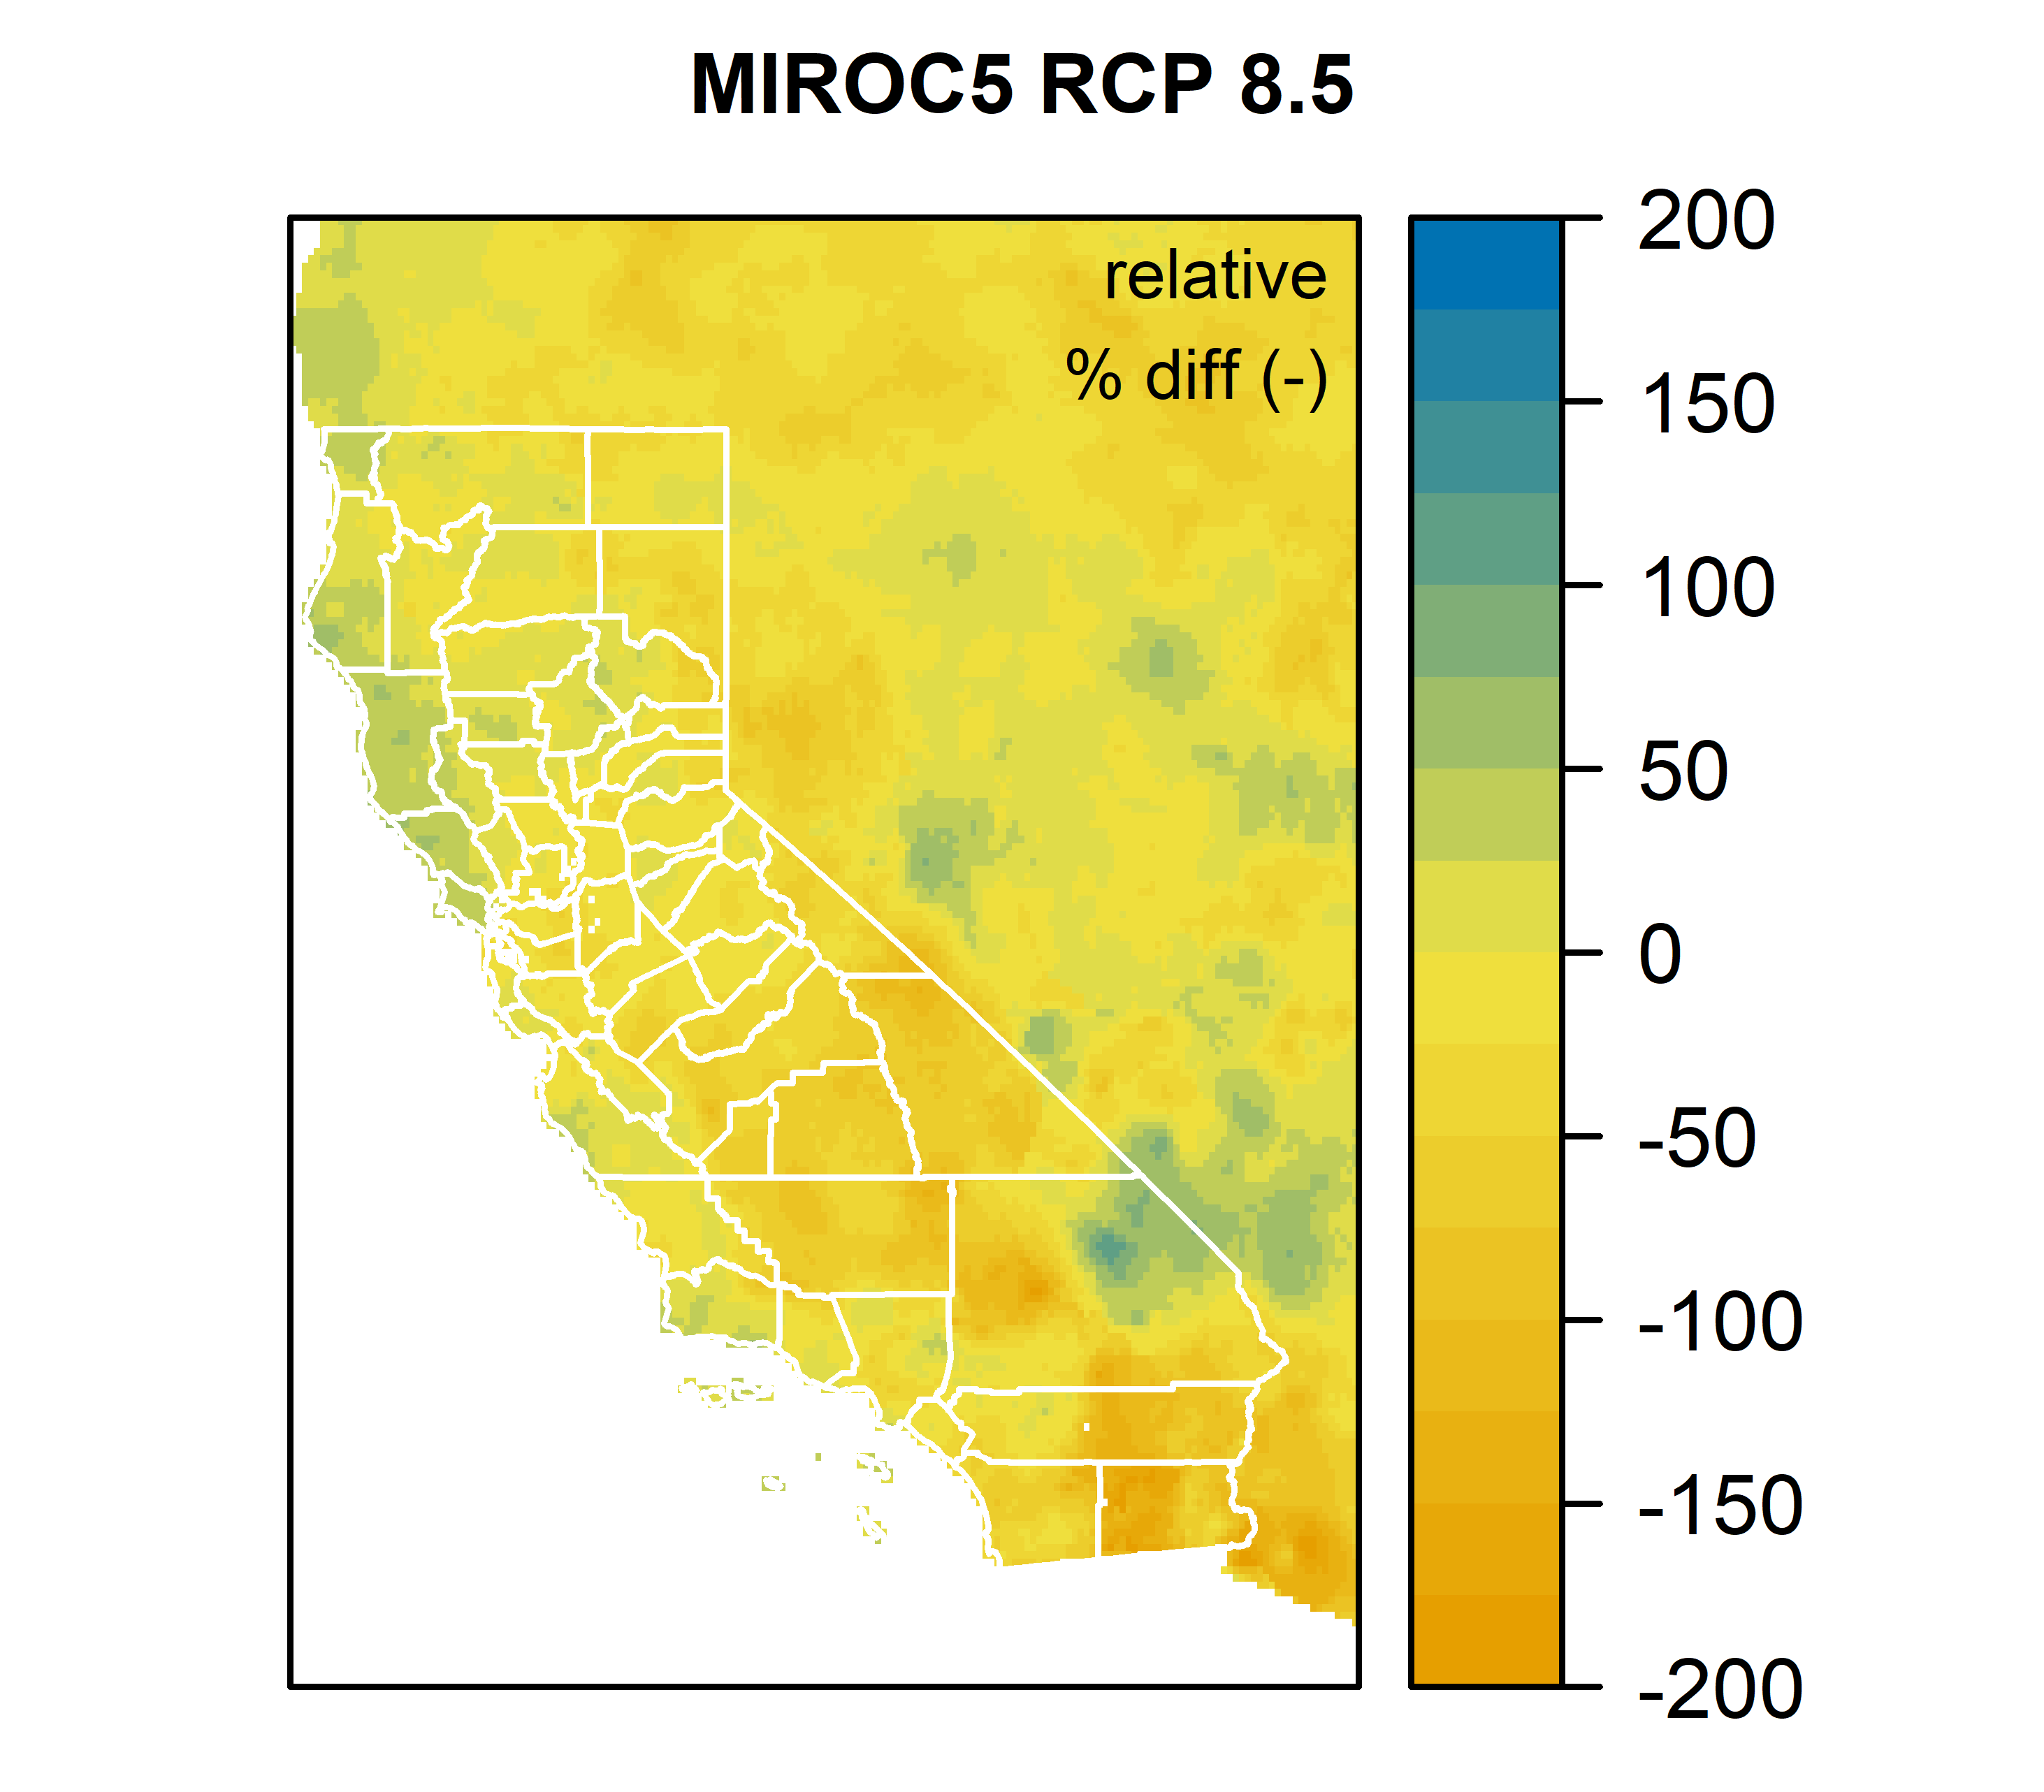
\includegraphics[width=.24\textwidth, trim={1cm 0 0 0}]{plots/rplot54_PPT_MIROC5_85_rpd.png}
    \caption[Relative percent difference in precipitation for each climate model.]{Relative percent difference in precipitation for each climate model. MIROC5 RCP 8.5 and CanESM2 RCP 4.5 show the most amount of dryness across California. In other models, southern California becomes wetter (e.g, CNRMCM5 RCP 4.5 and HadGEM2ES 4.5). This projected wetness can be viewed as a southward shift in the cooler/wetter climates of today. In all models, except for CanESM2, the RCP 8.5 scenario is dryer than its counter part RCP 4.5. }
    \label{fig:rpdmap_ppt}
\end{figure}

\begin{figure}
    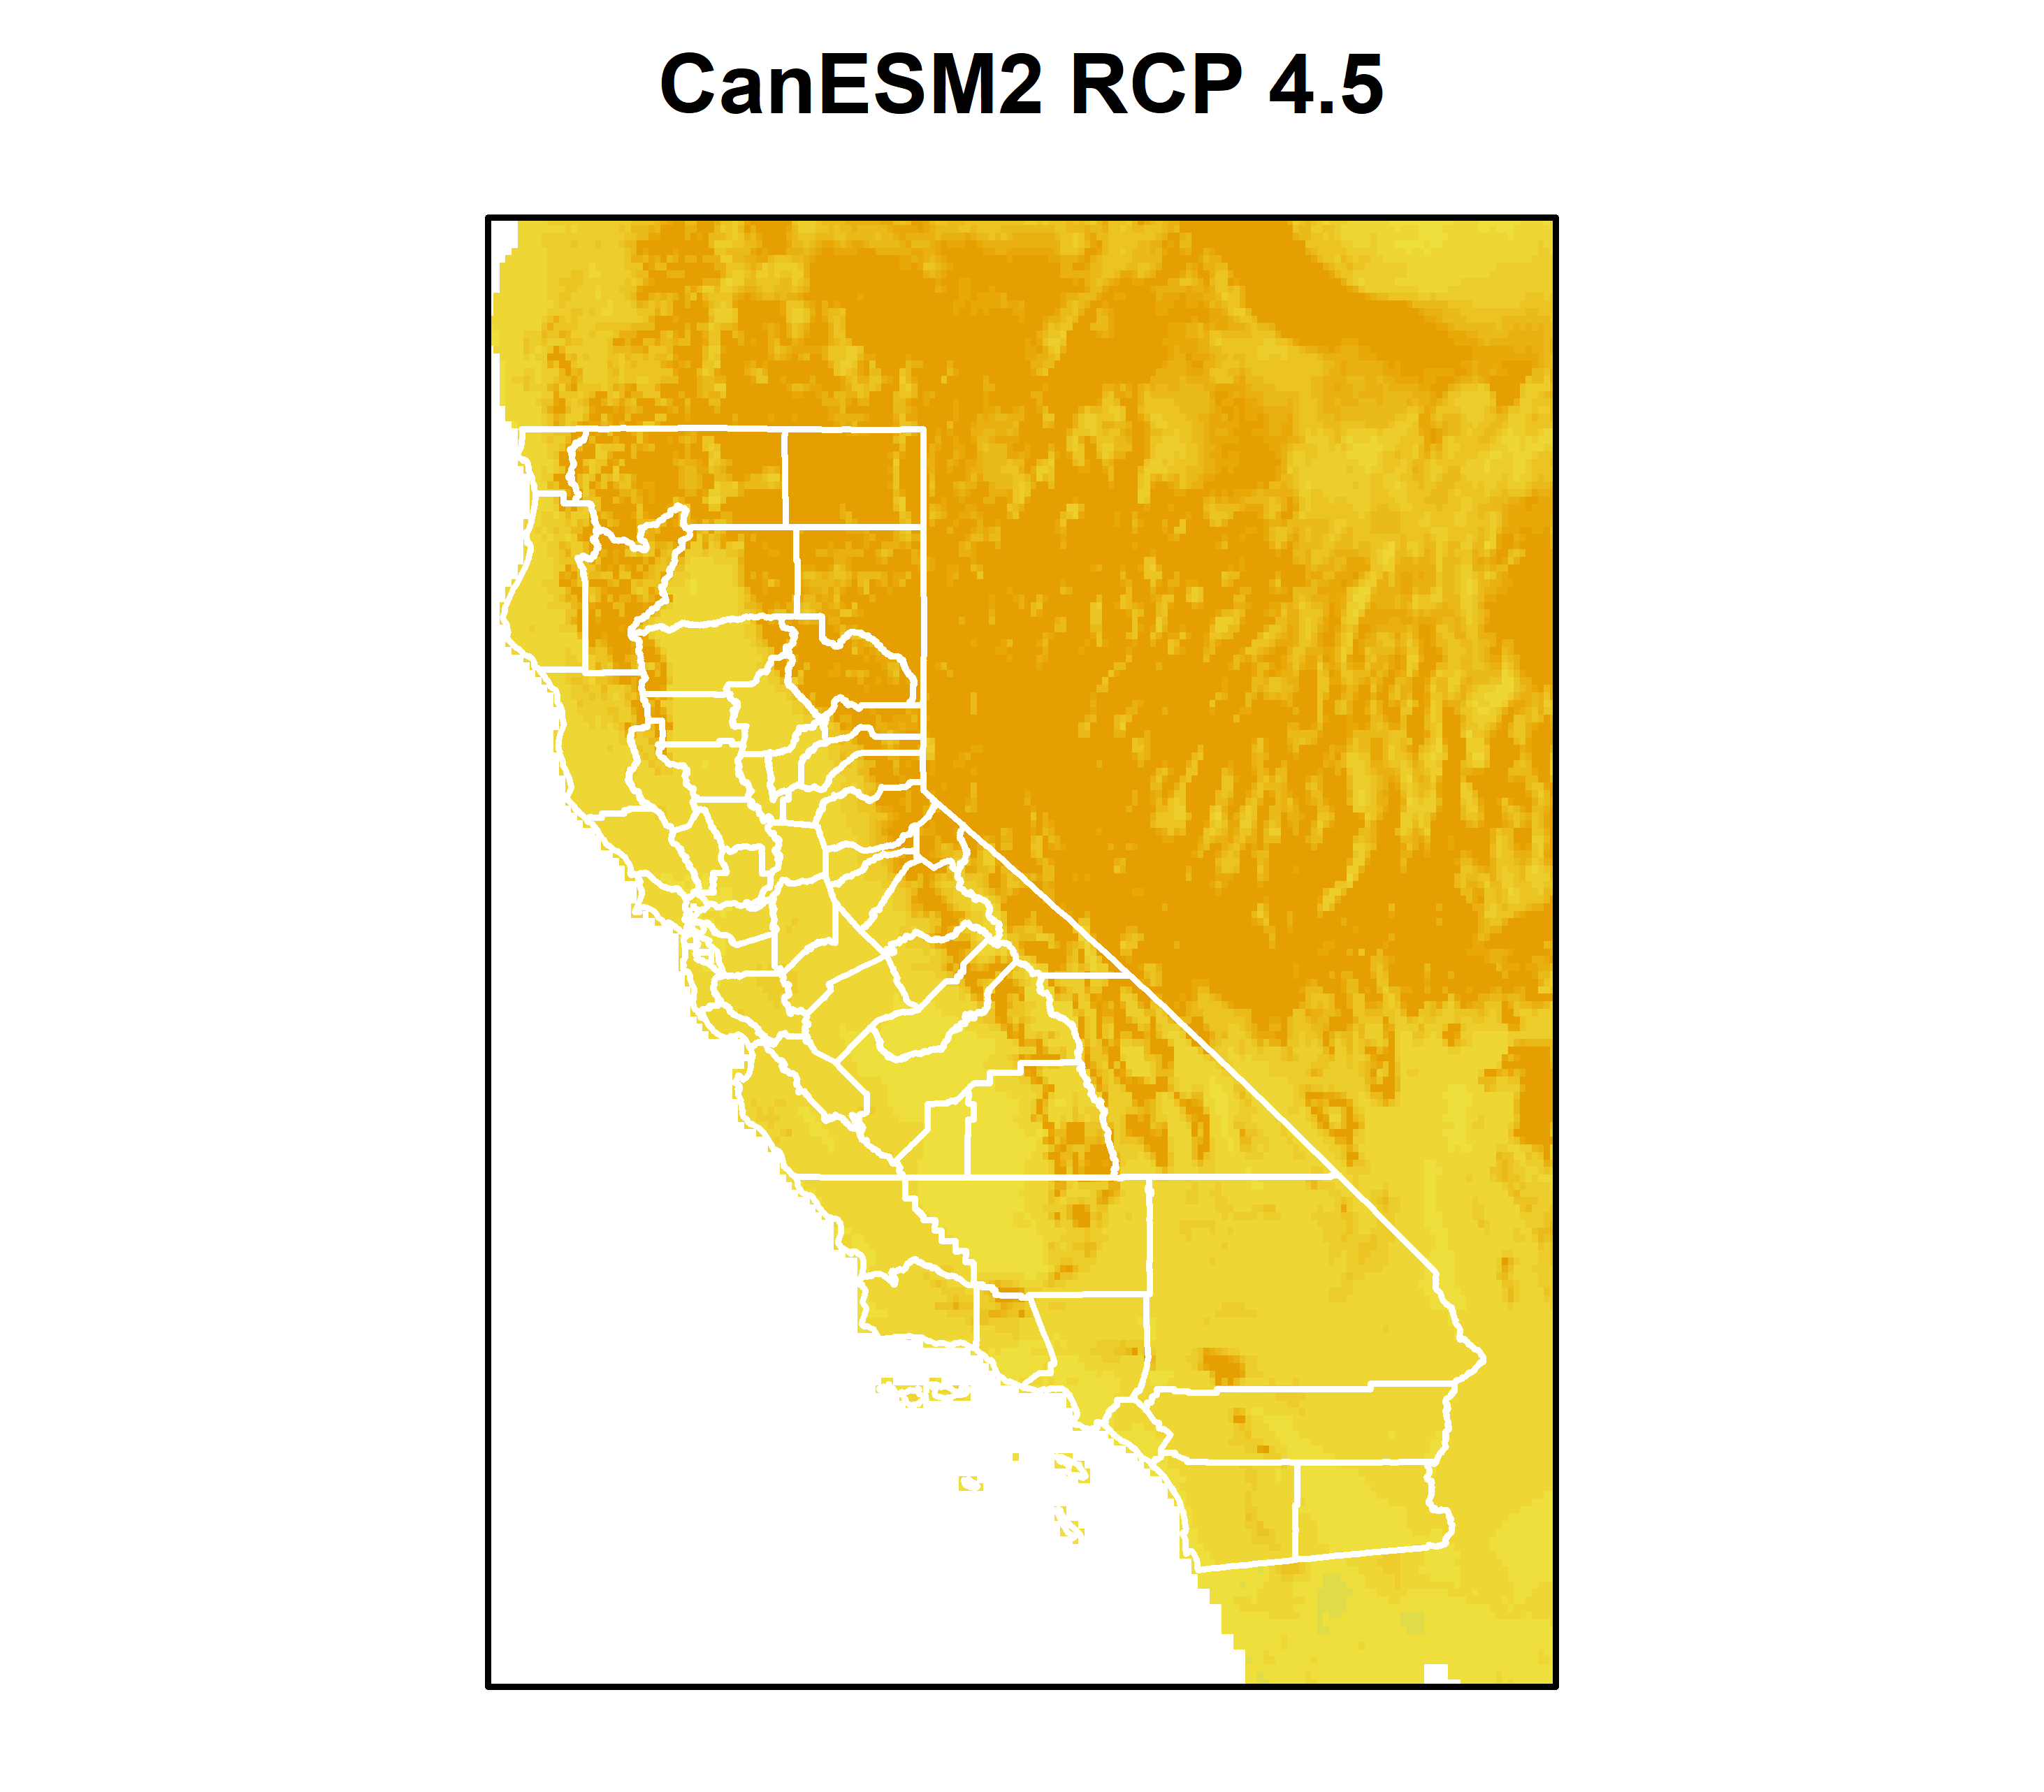
\includegraphics[width=.24\textwidth, trim={1cm 0 0 0}]{plots/rplot54_TMP_CanESM2_45_rpd.png}\hfill
    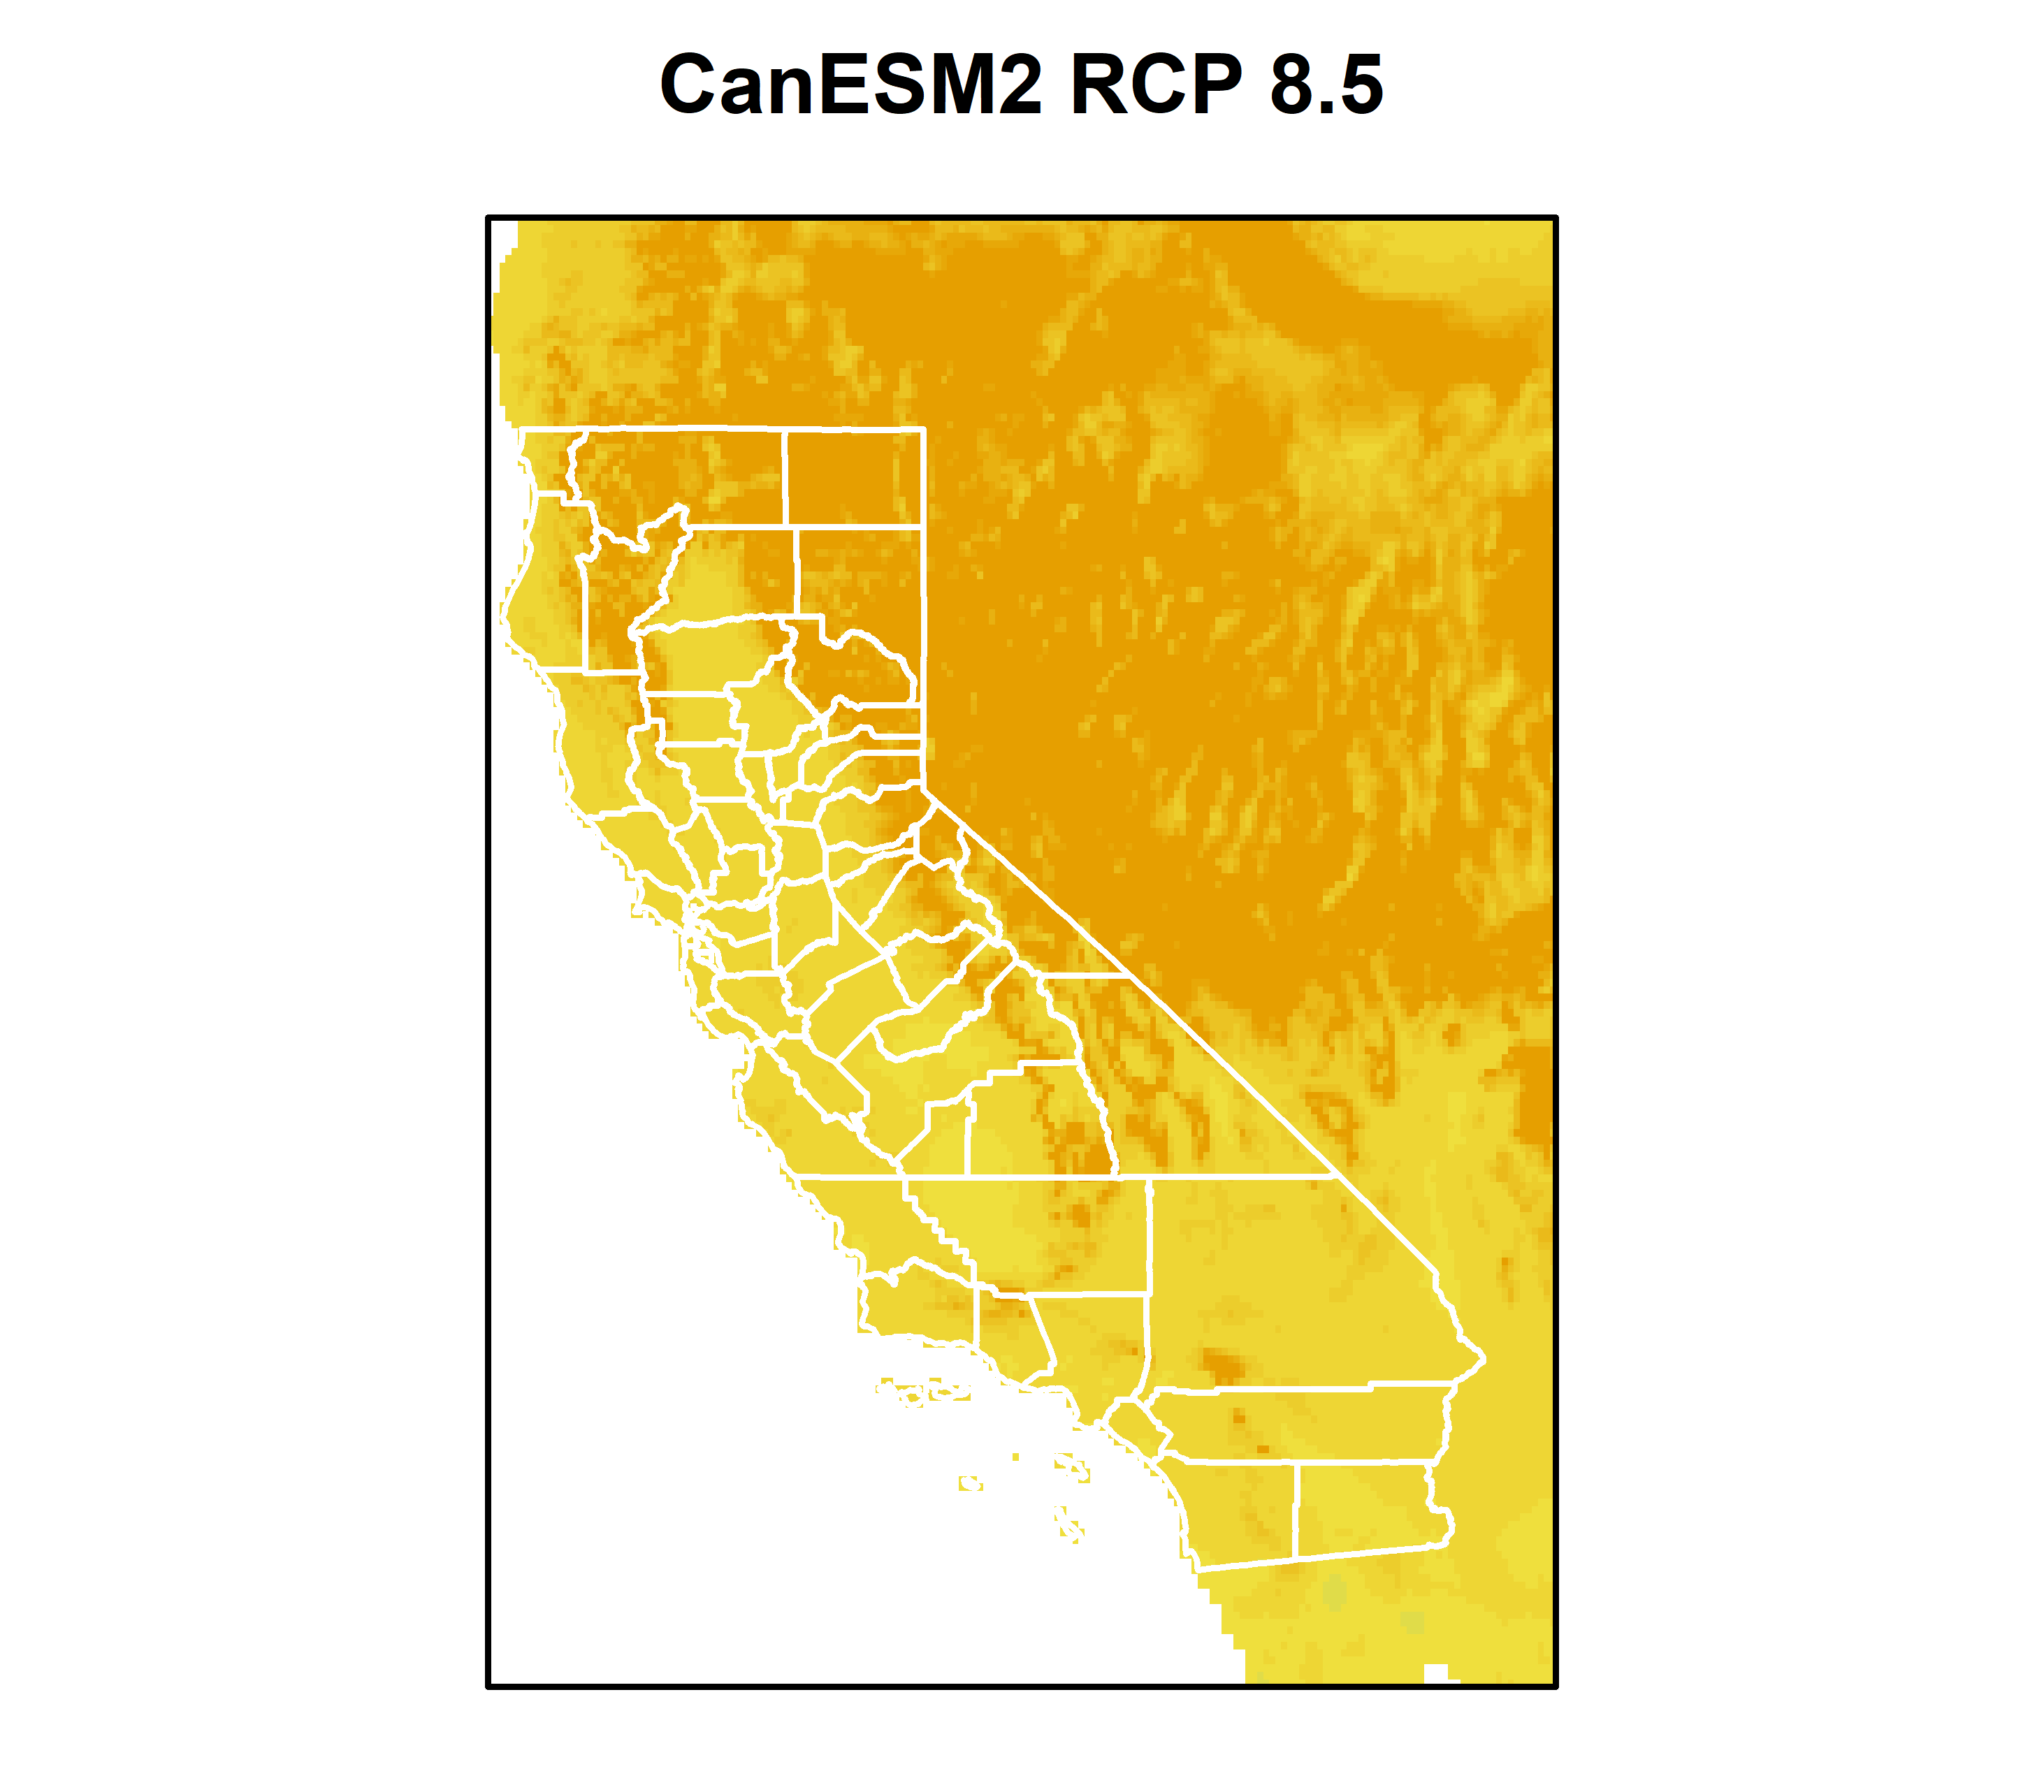
\includegraphics[width=.24\textwidth, trim={1cm 0 0 0}]{plots/rplot54_TMP_CanESM2_85_rpd.png}\hfill
    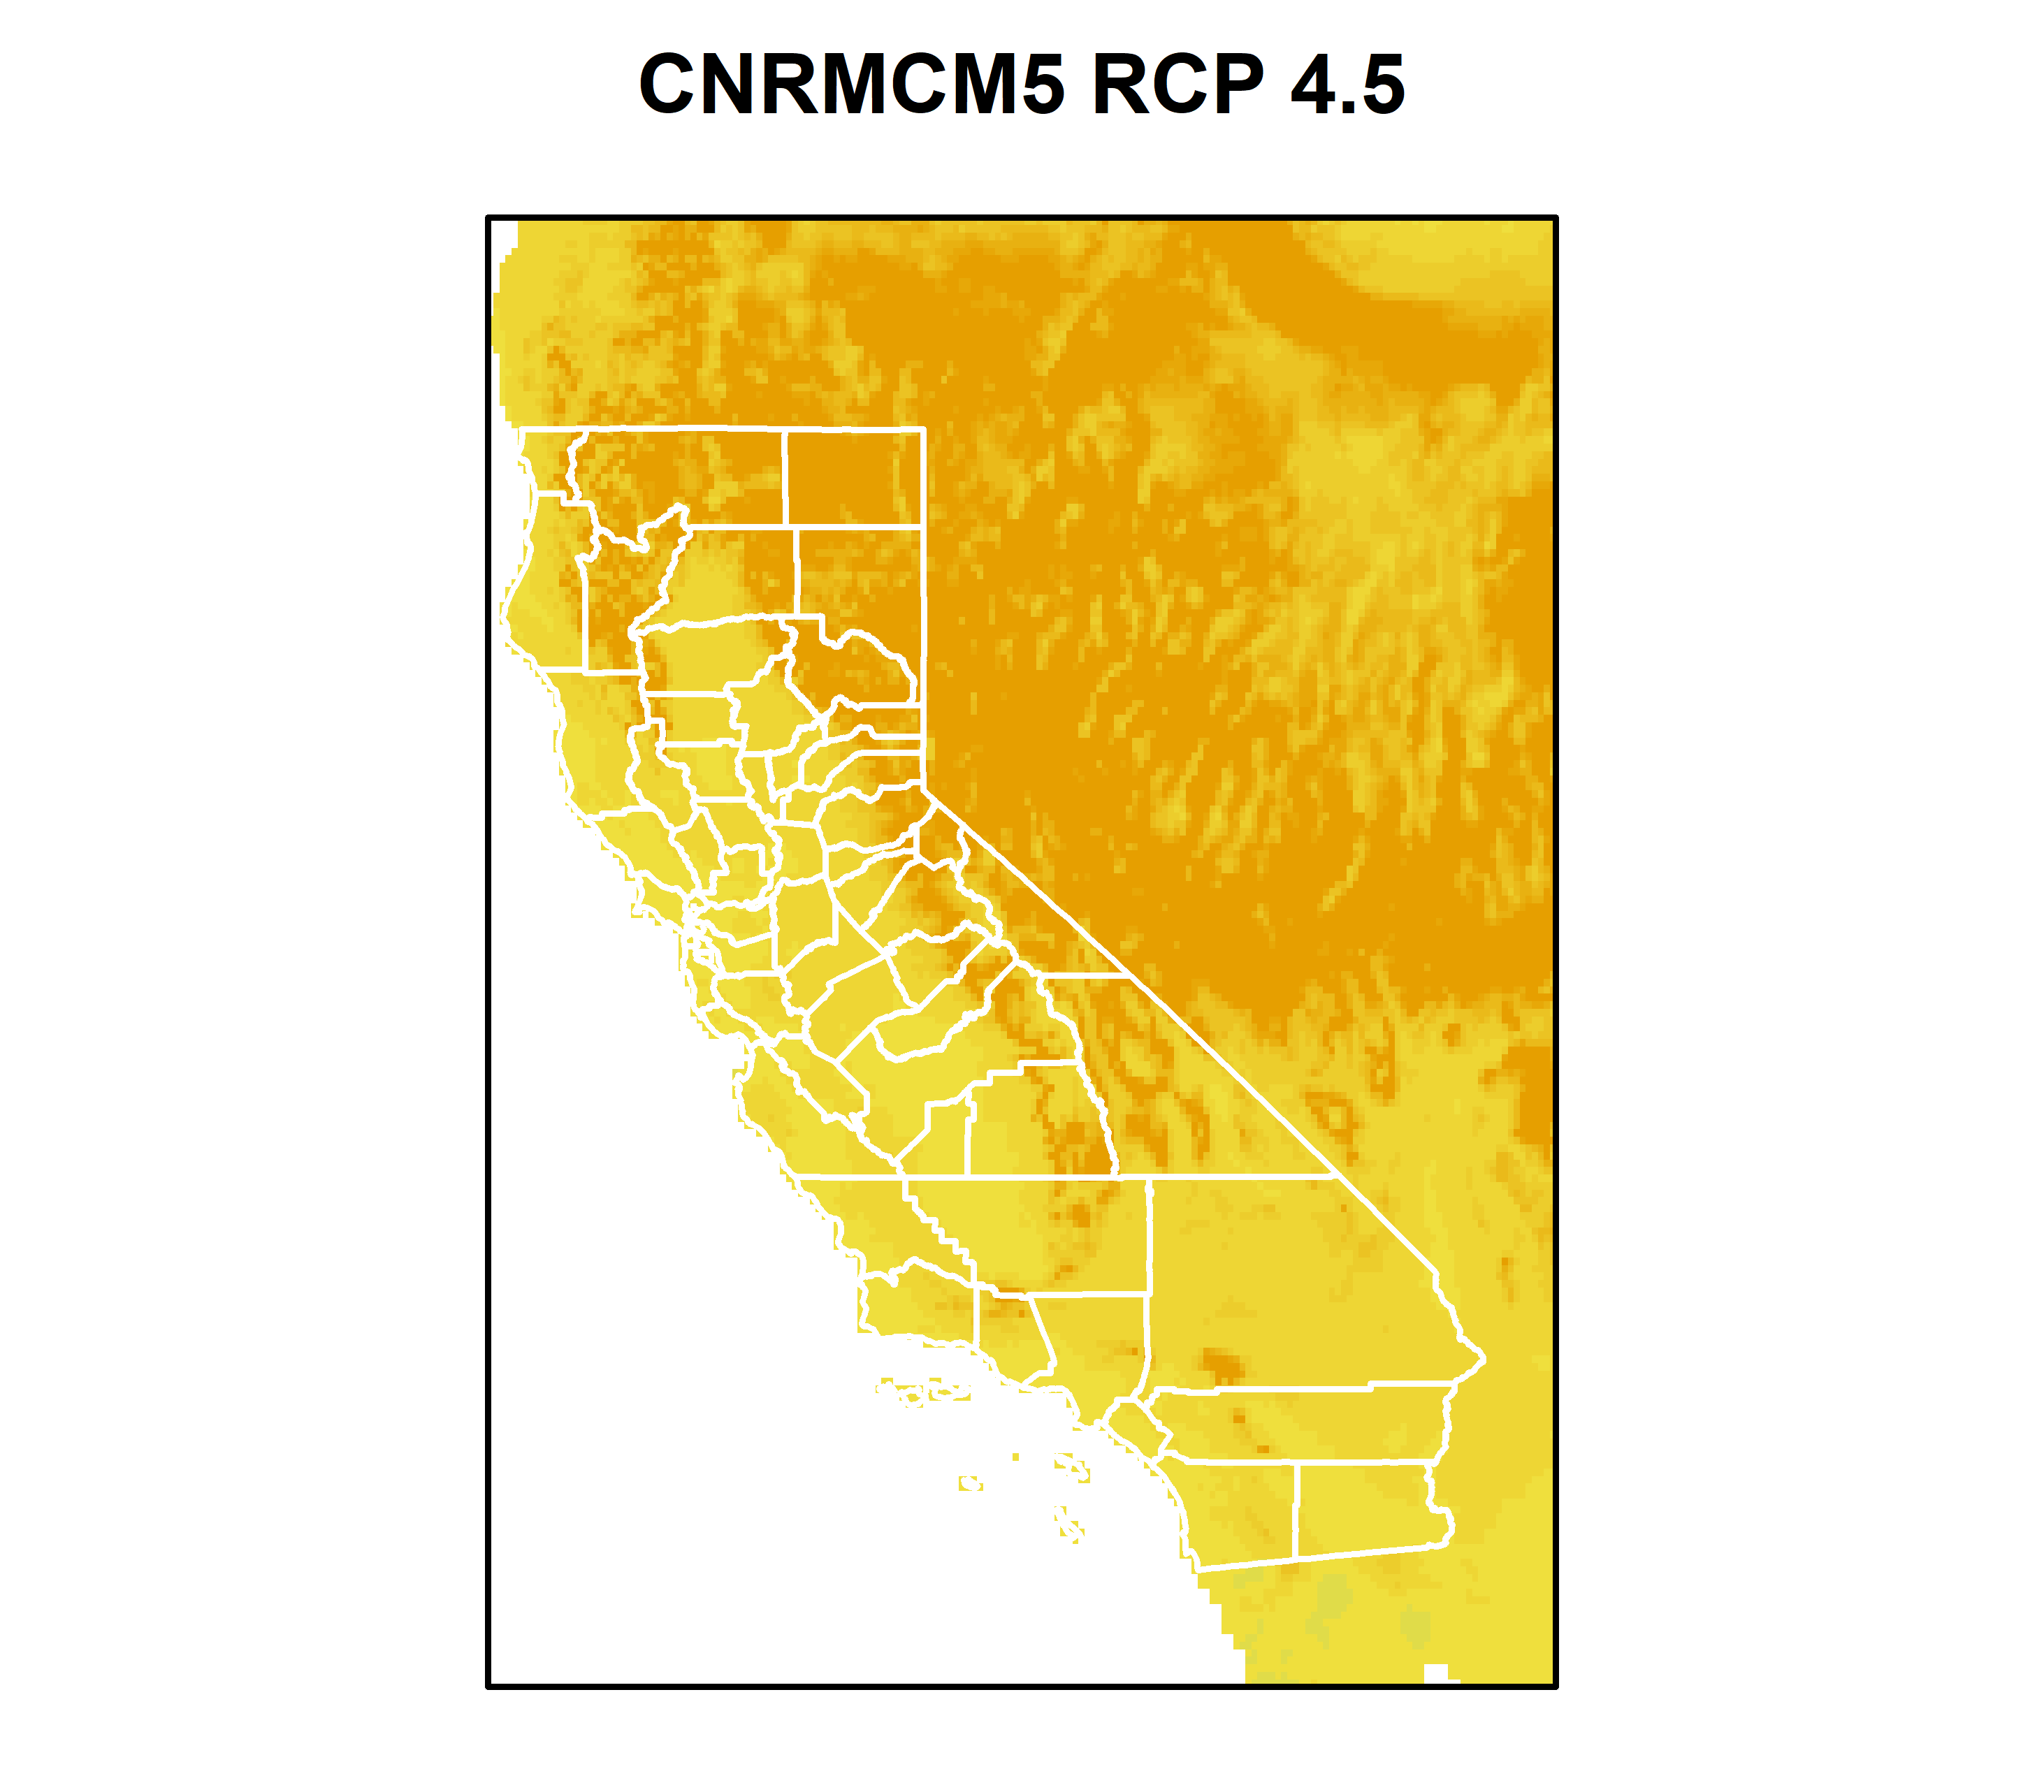
\includegraphics[width=.24\textwidth, trim={1cm 0 0 0}]{plots/rplot54_TMP_CNRMCM5_45_rpd.png}\hfill
    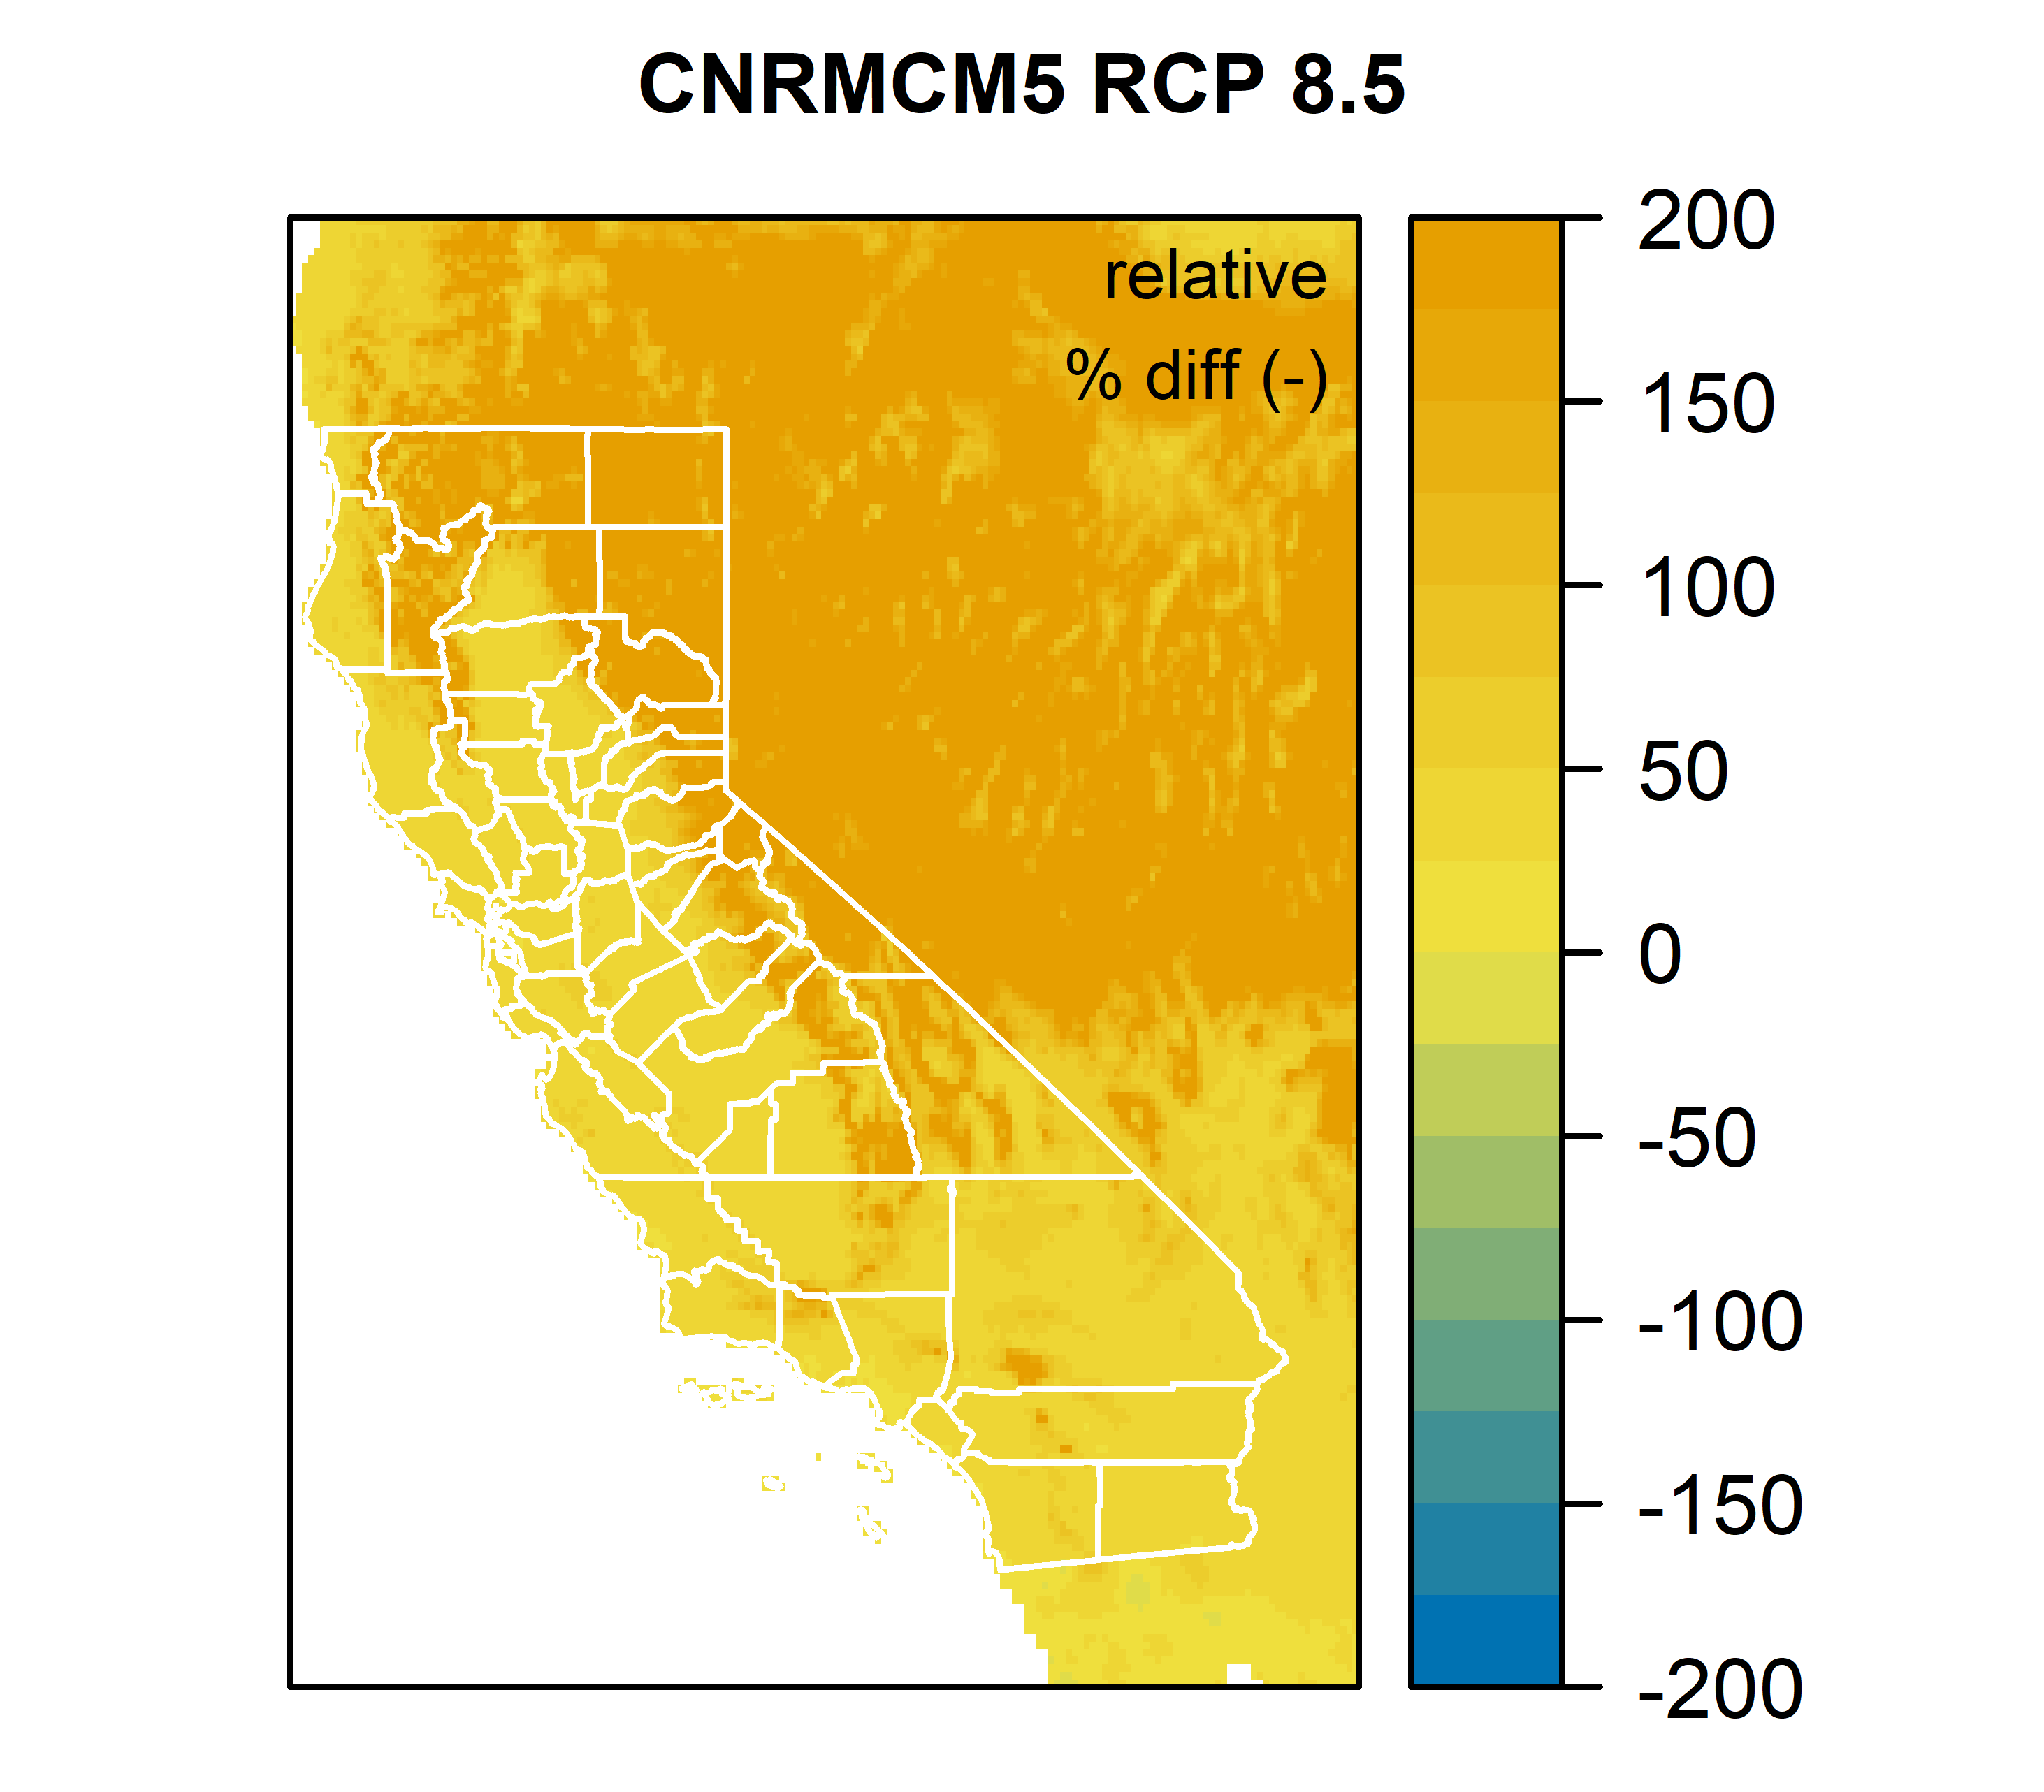
\includegraphics[width=.24\textwidth, trim={1cm 0 0 0}]{plots/rplot54_TMP_CNRMCM5_85_rpd.png}
    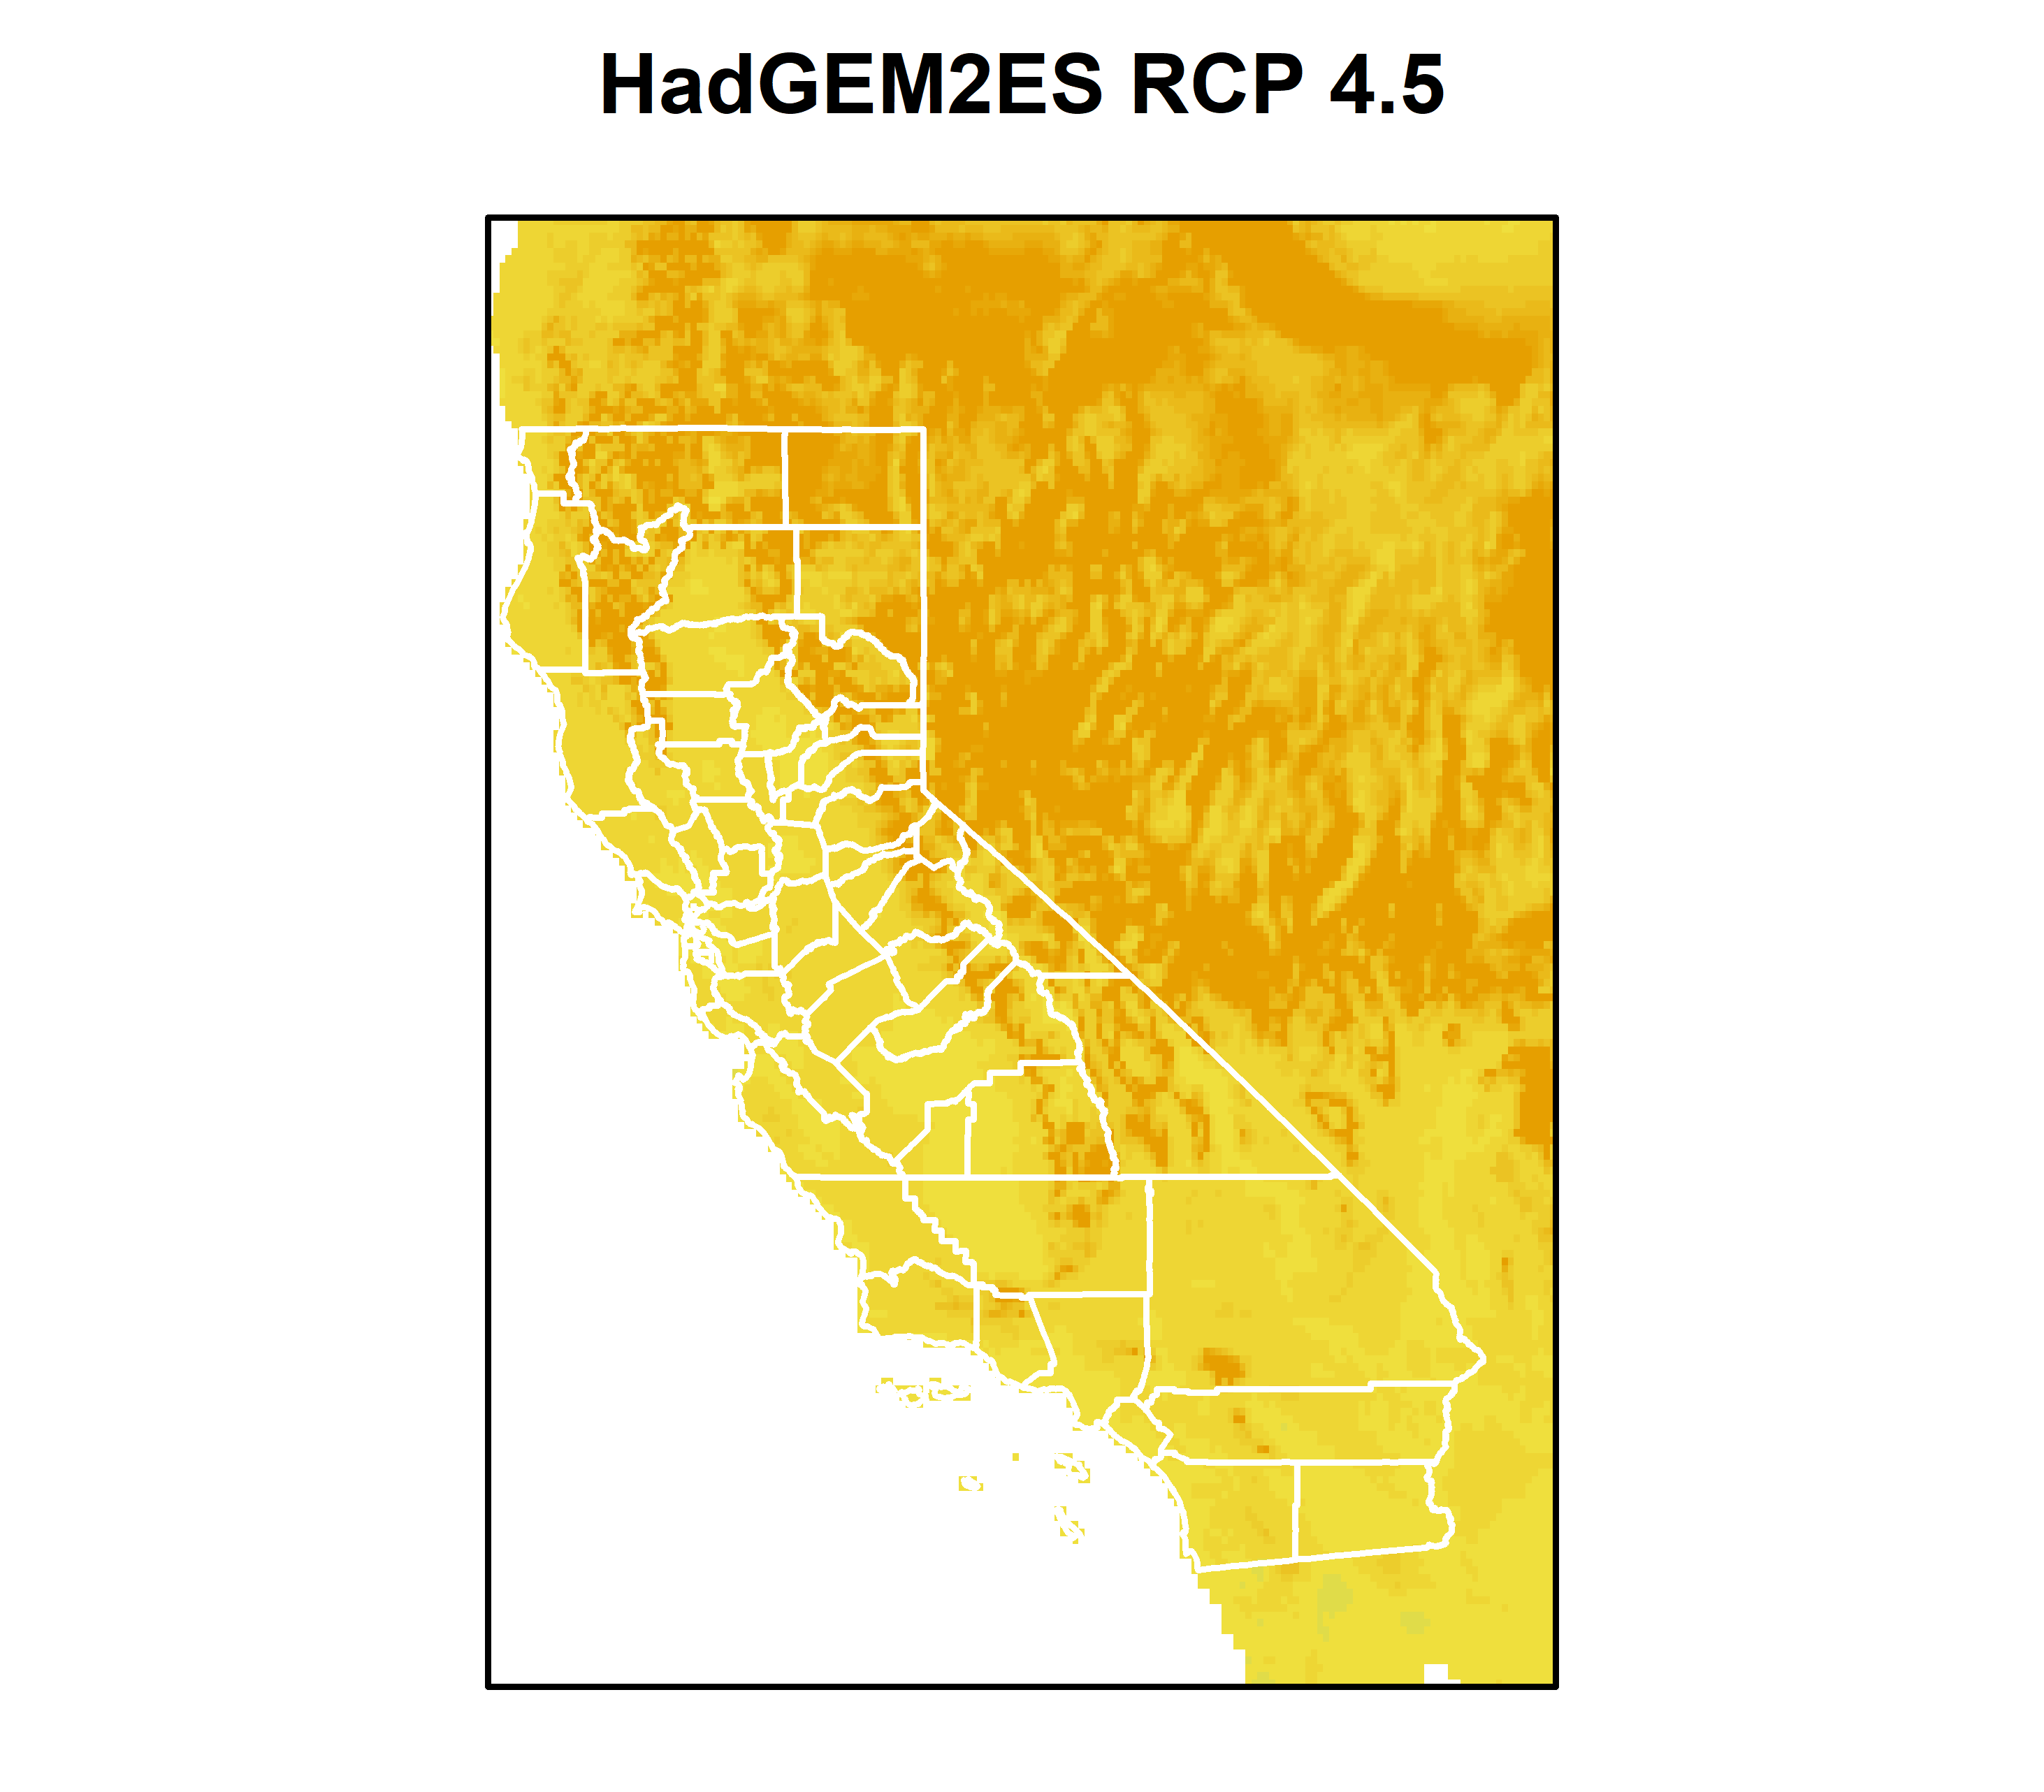
\includegraphics[width=.24\textwidth, trim={1cm 0 0 0}]{plots/rplot54_TMP_HadGEM2ES_45_rpd.png}\hfill
    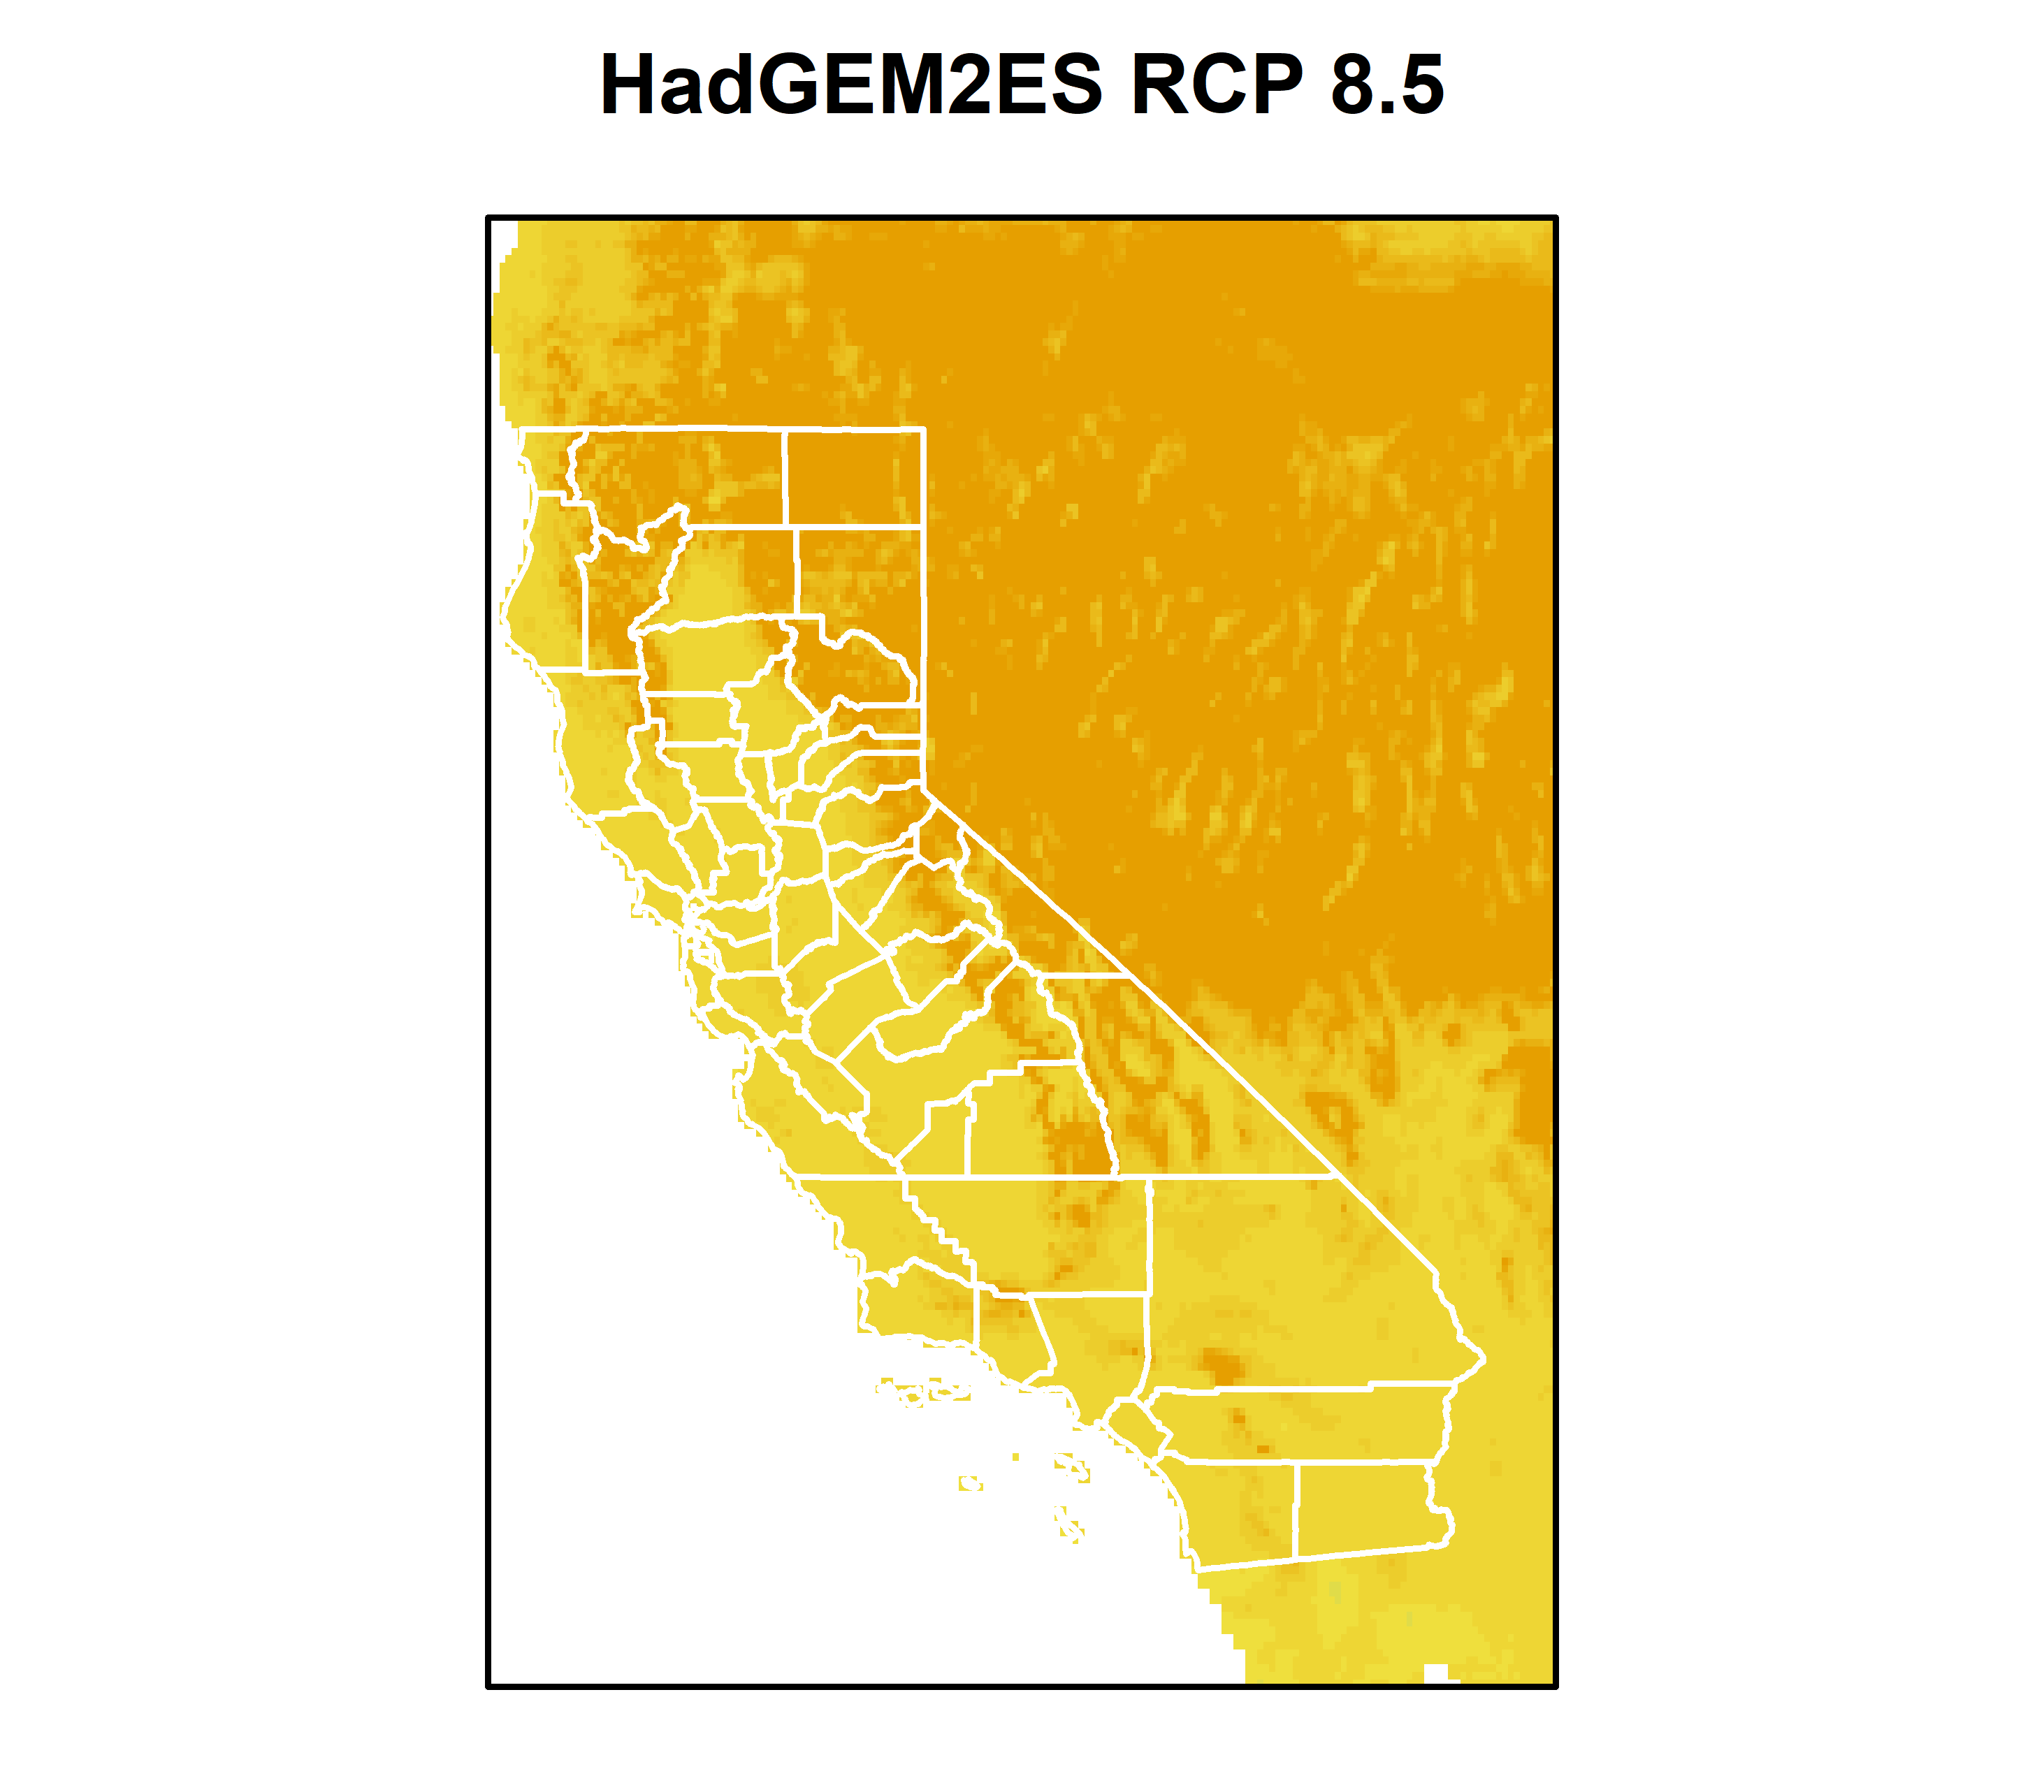
\includegraphics[width=.24\textwidth, trim={1cm 0 0 0}]{plots/rplot54_TMP_HadGEM2ES_85_rpd.png}\hfill
    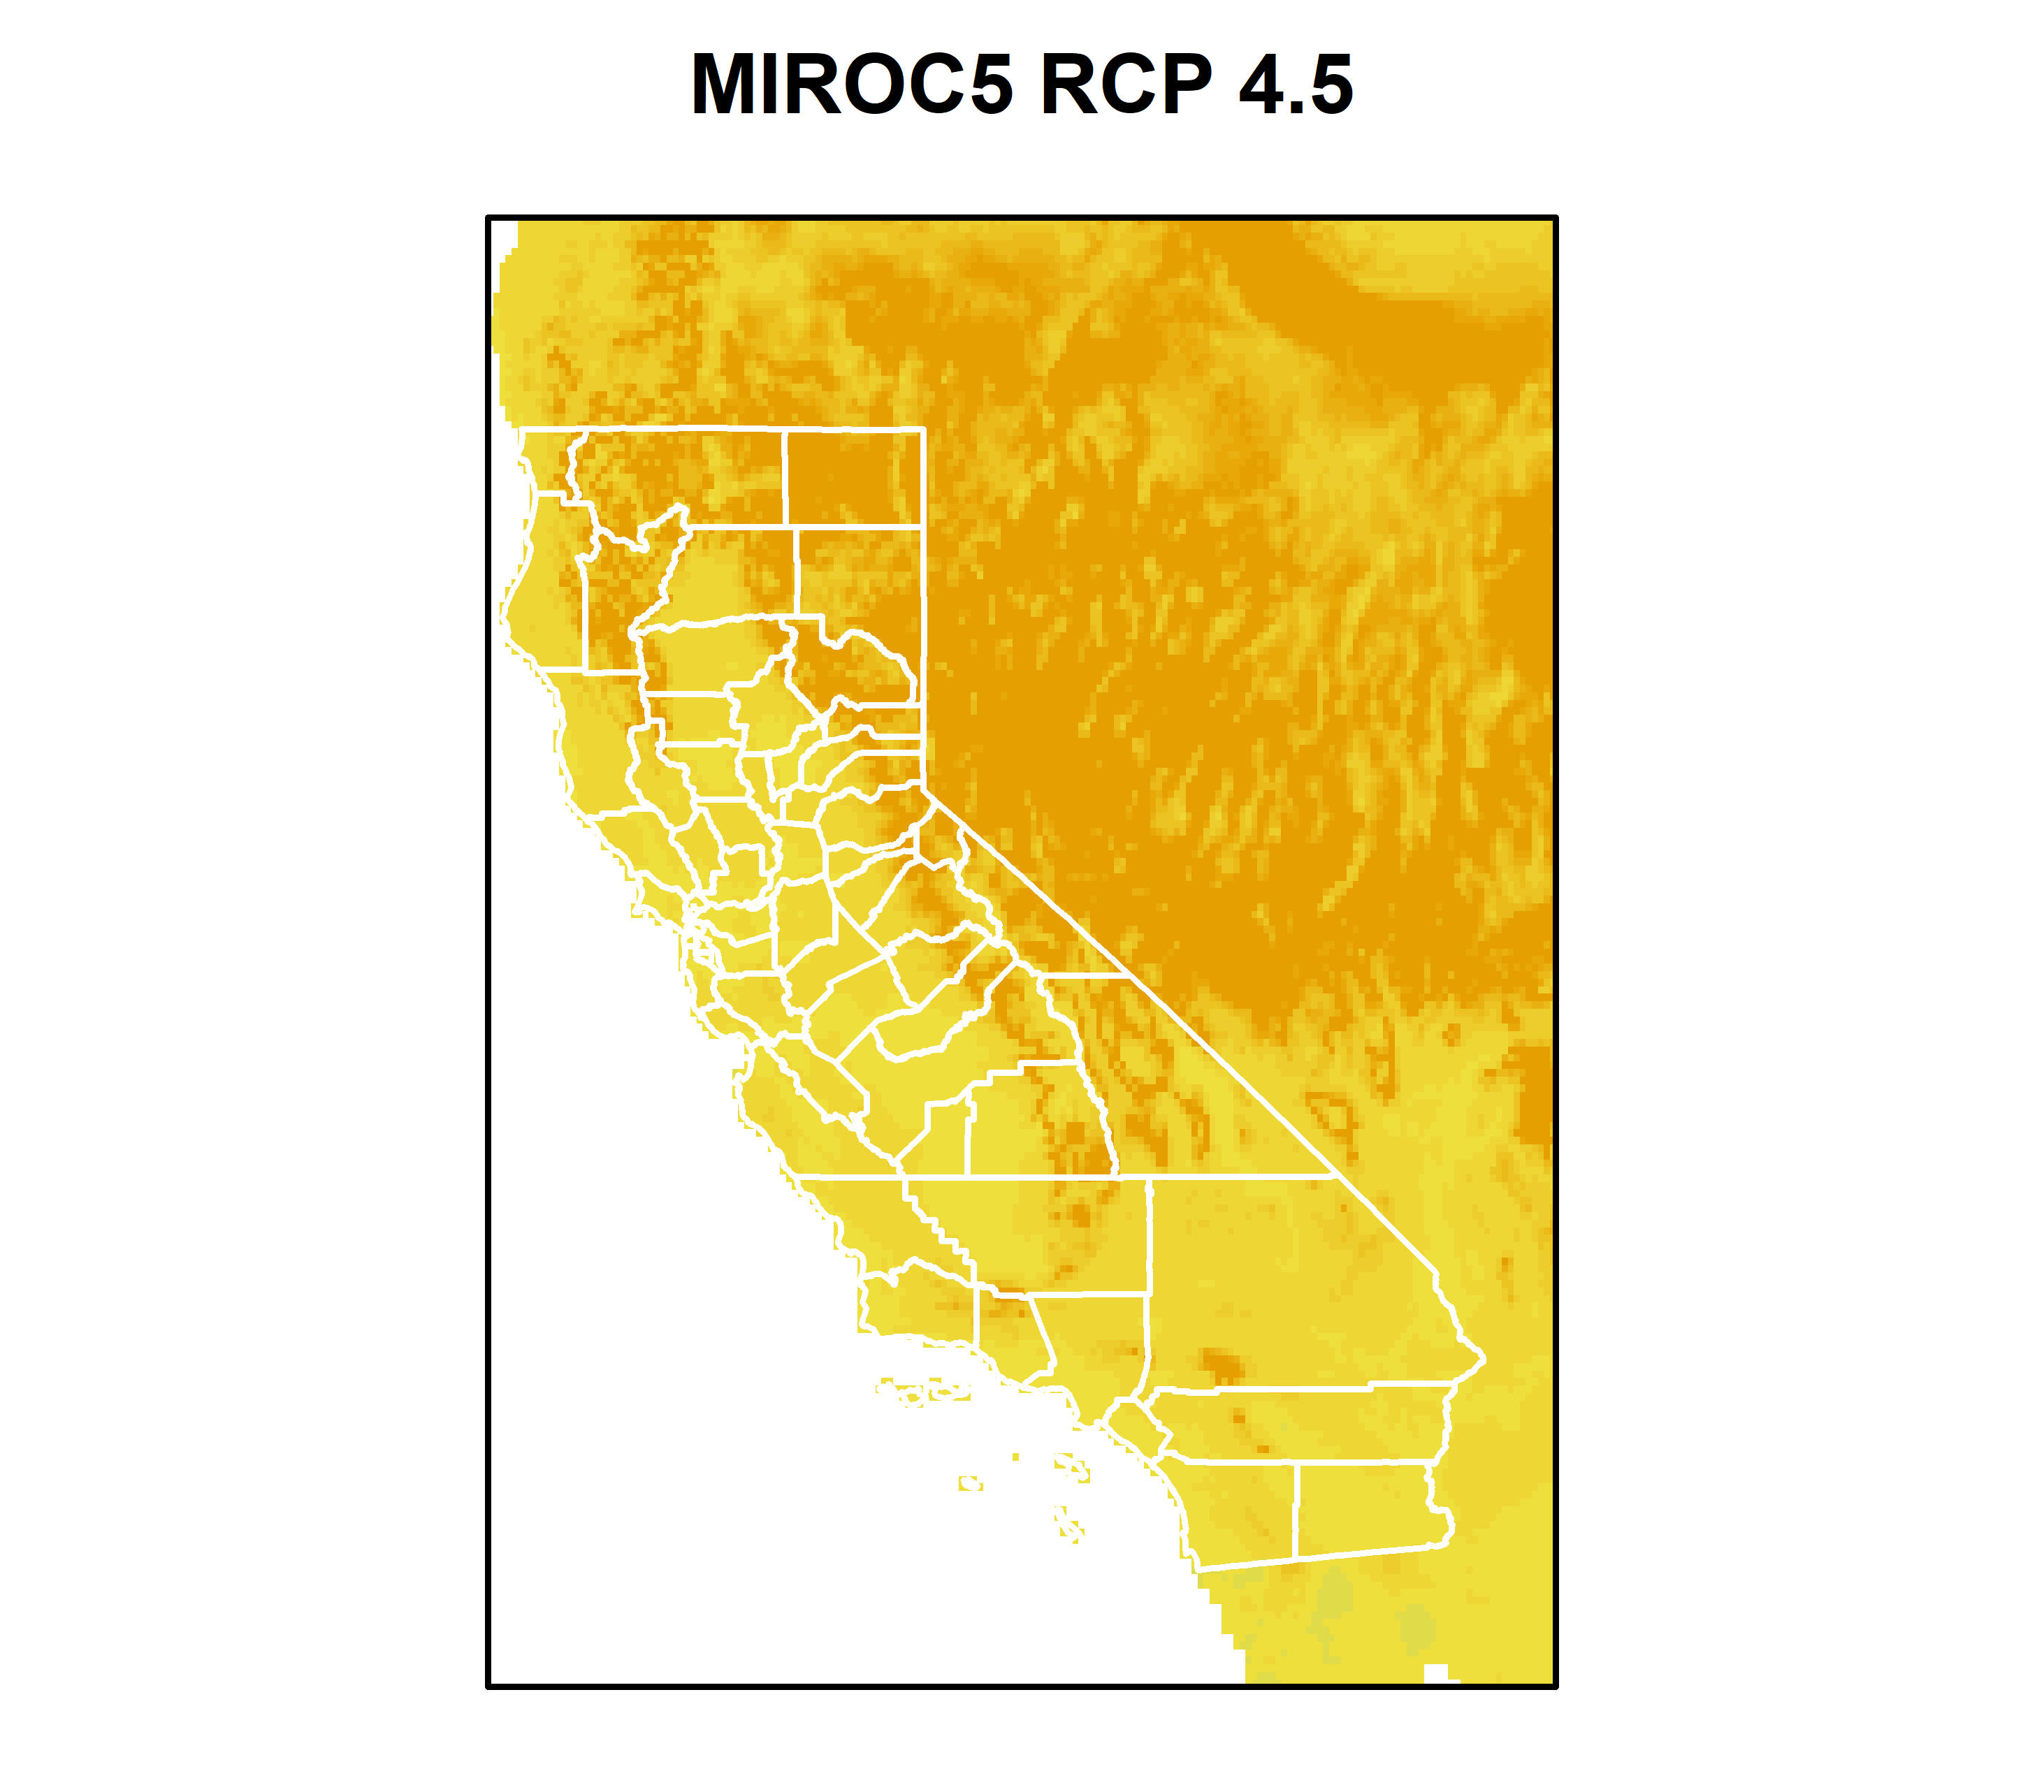
\includegraphics[width=.24\textwidth, trim={1cm 0 0 0}]{plots/rplot54_TMP_MIROC5_45_rpd.png}\hfill
    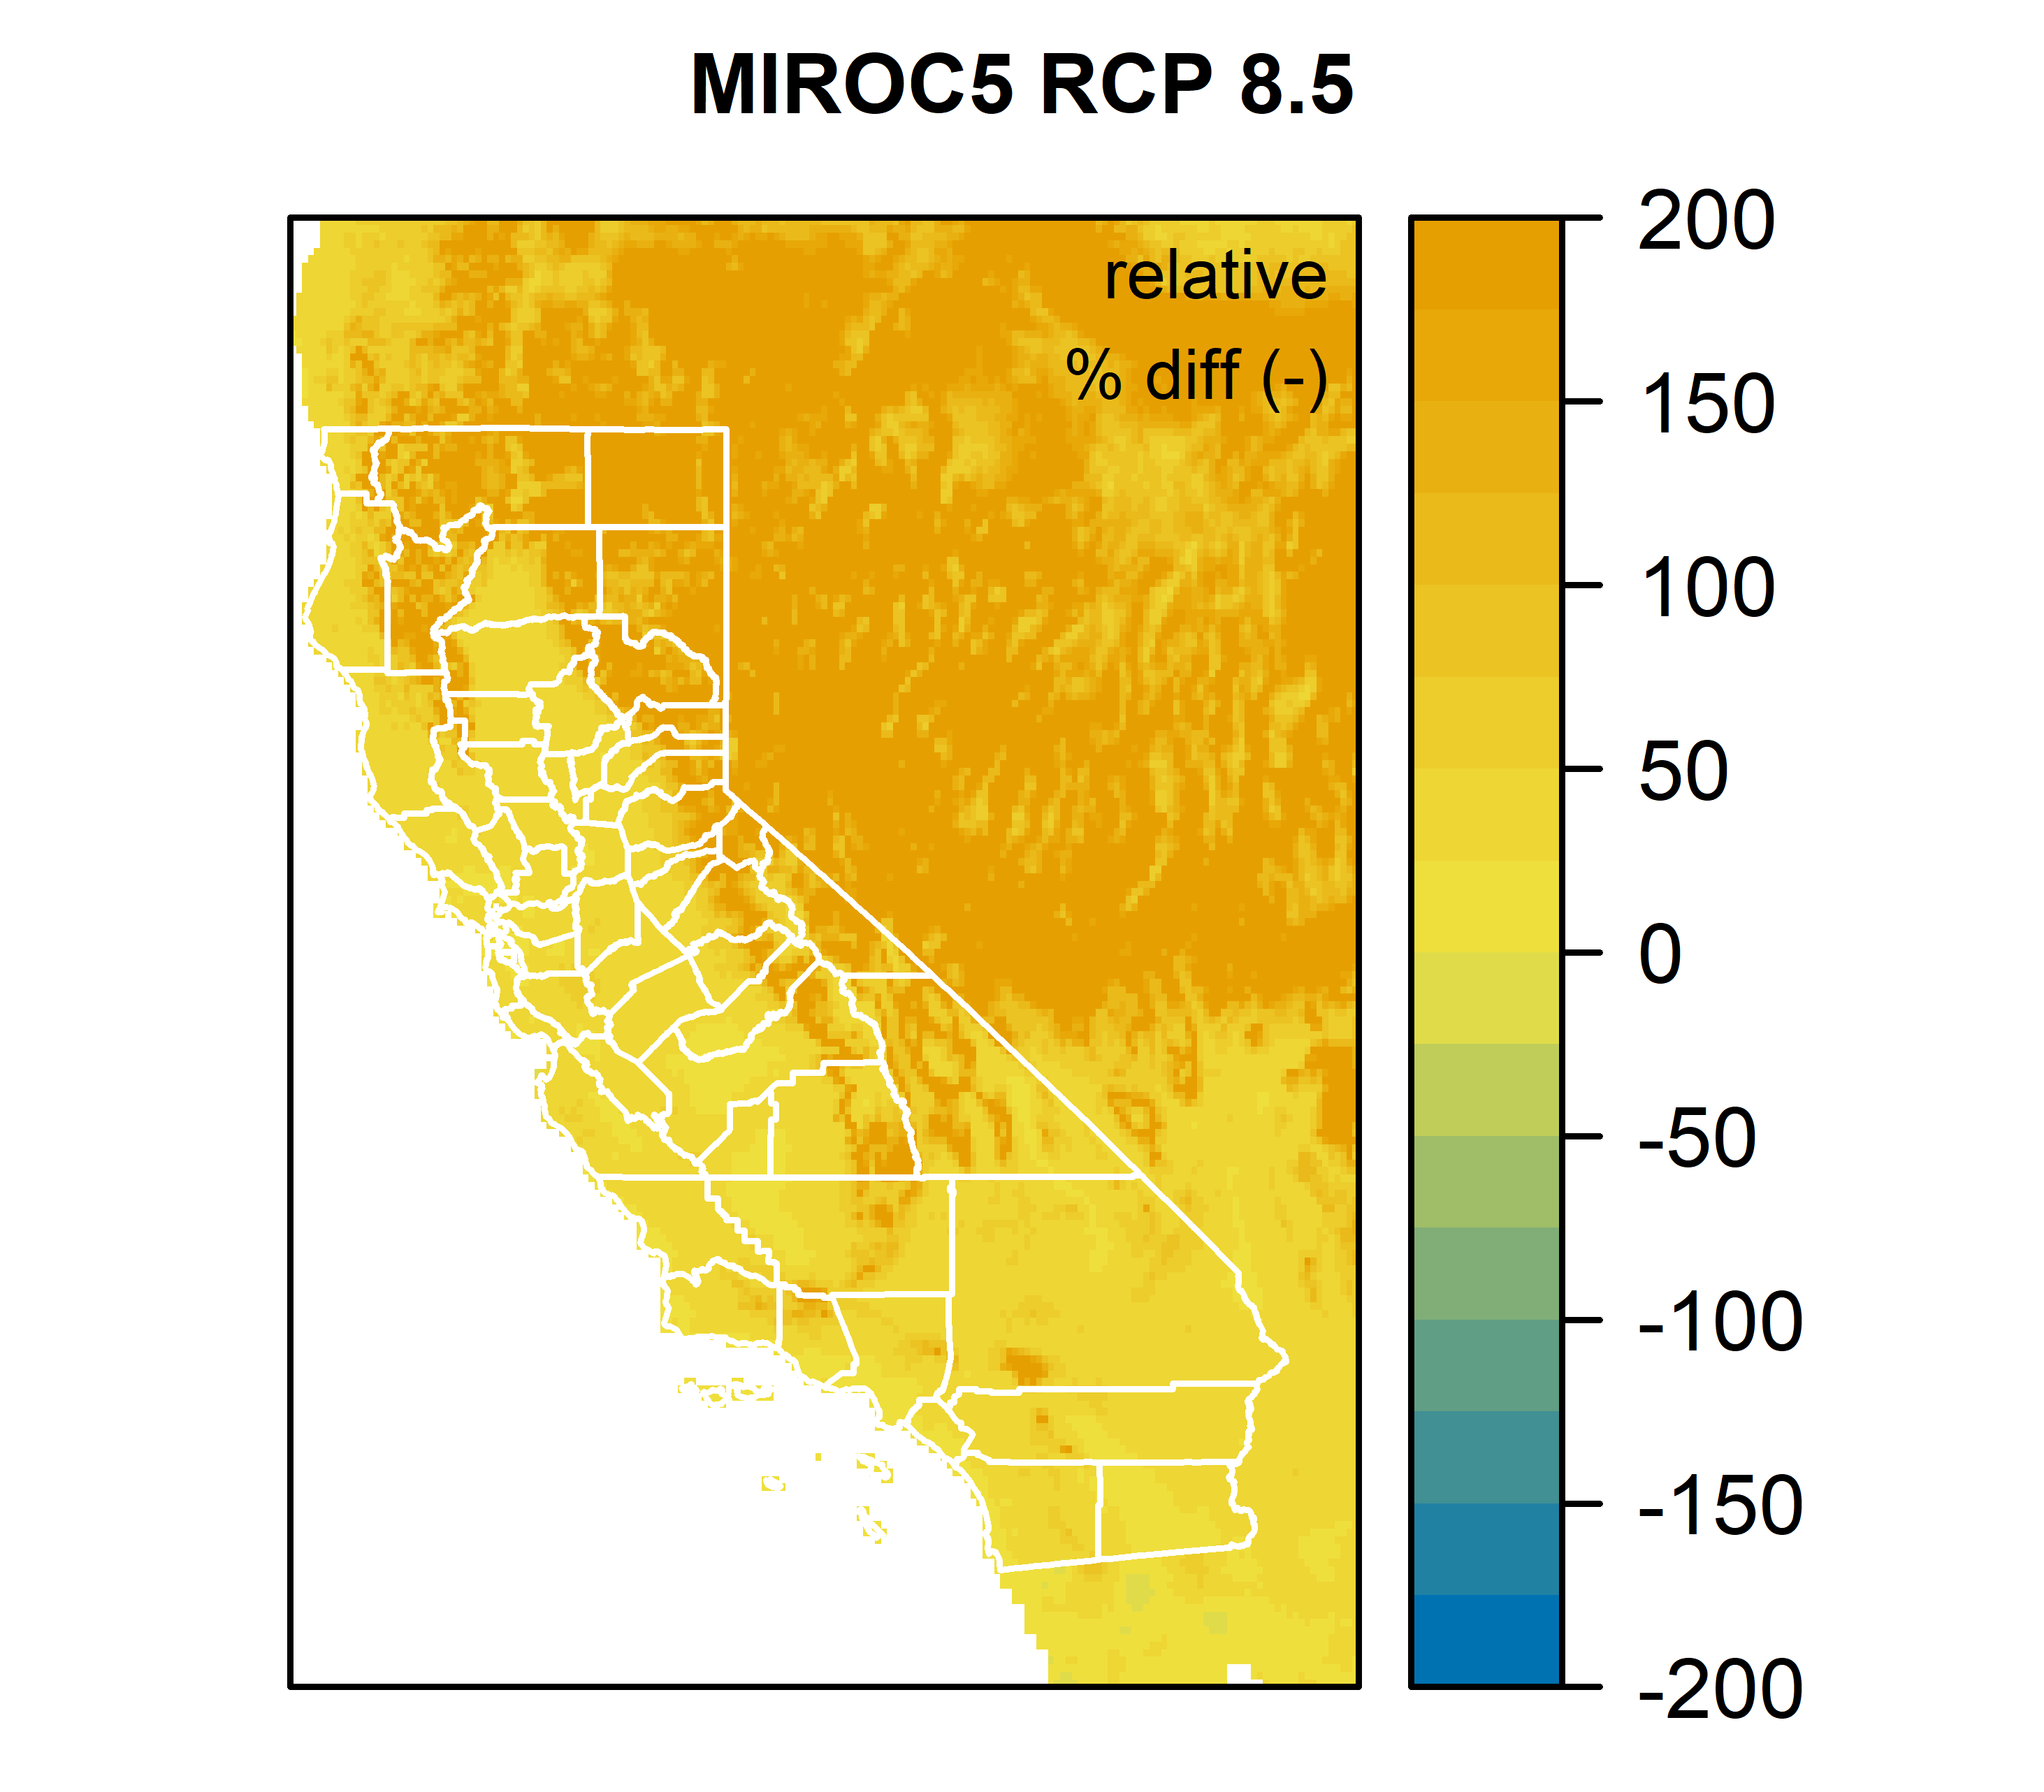
\includegraphics[width=.24\textwidth, trim={1cm 0 0 0}]{plots/rplot54_TMP_MIROC5_85_rpd.png}
    \caption[Relative percent difference in air temperature for each climate model.]{Relative percent difference in air temperature for each climate model. In all models, California becomes hotter in all areas of the state; the relative percent difference is never negative. The Sierra-Nevada range and the northern part of California are projected to experience the brunt of the warming and the central valley and southern California are projected warm to a lesser extent. In all models, the RCP 8.5 scenario is slightly hotter than its counterpart RCP 4.5. Overall, there is more agreement between the models on air temperature changes than there is with precipitation.}
    \label{fig:rpdmap_tmp}
\end{figure}

\begin{figure}
    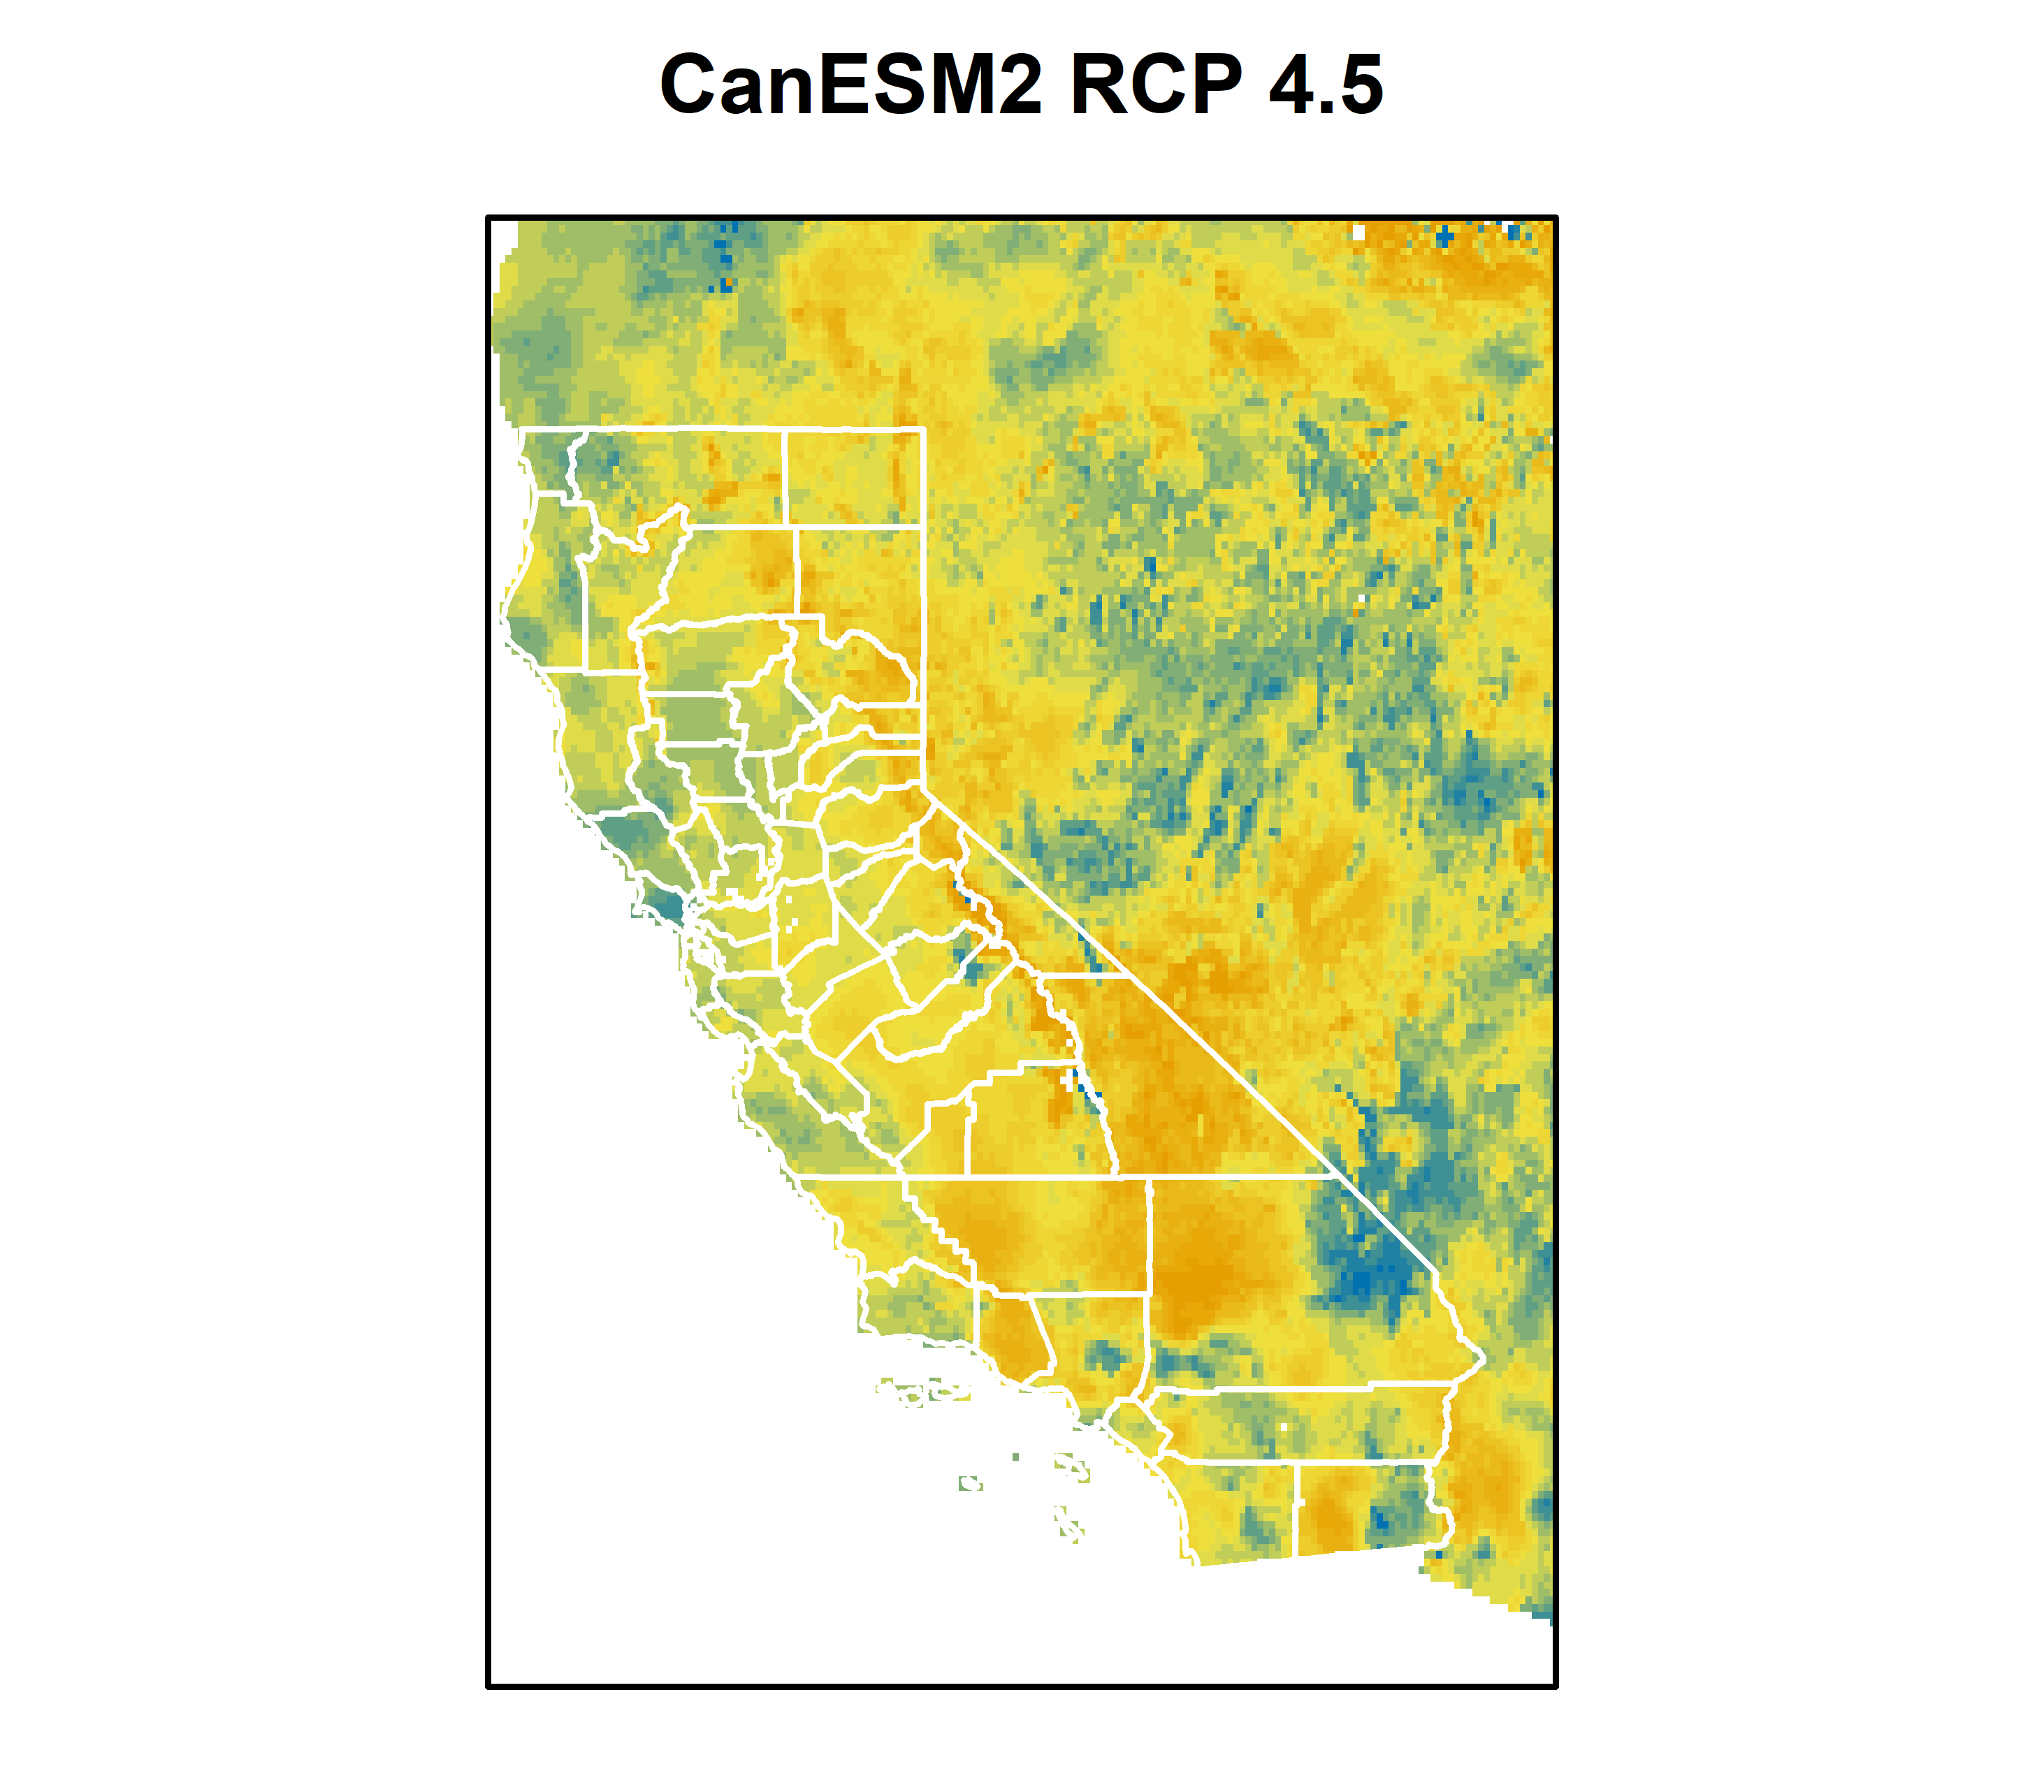
\includegraphics[width=.24\textwidth, trim={1cm 0 0 0}]{plots/rplot54_RNF_CanESM2_45_rpd.png}\hfill
    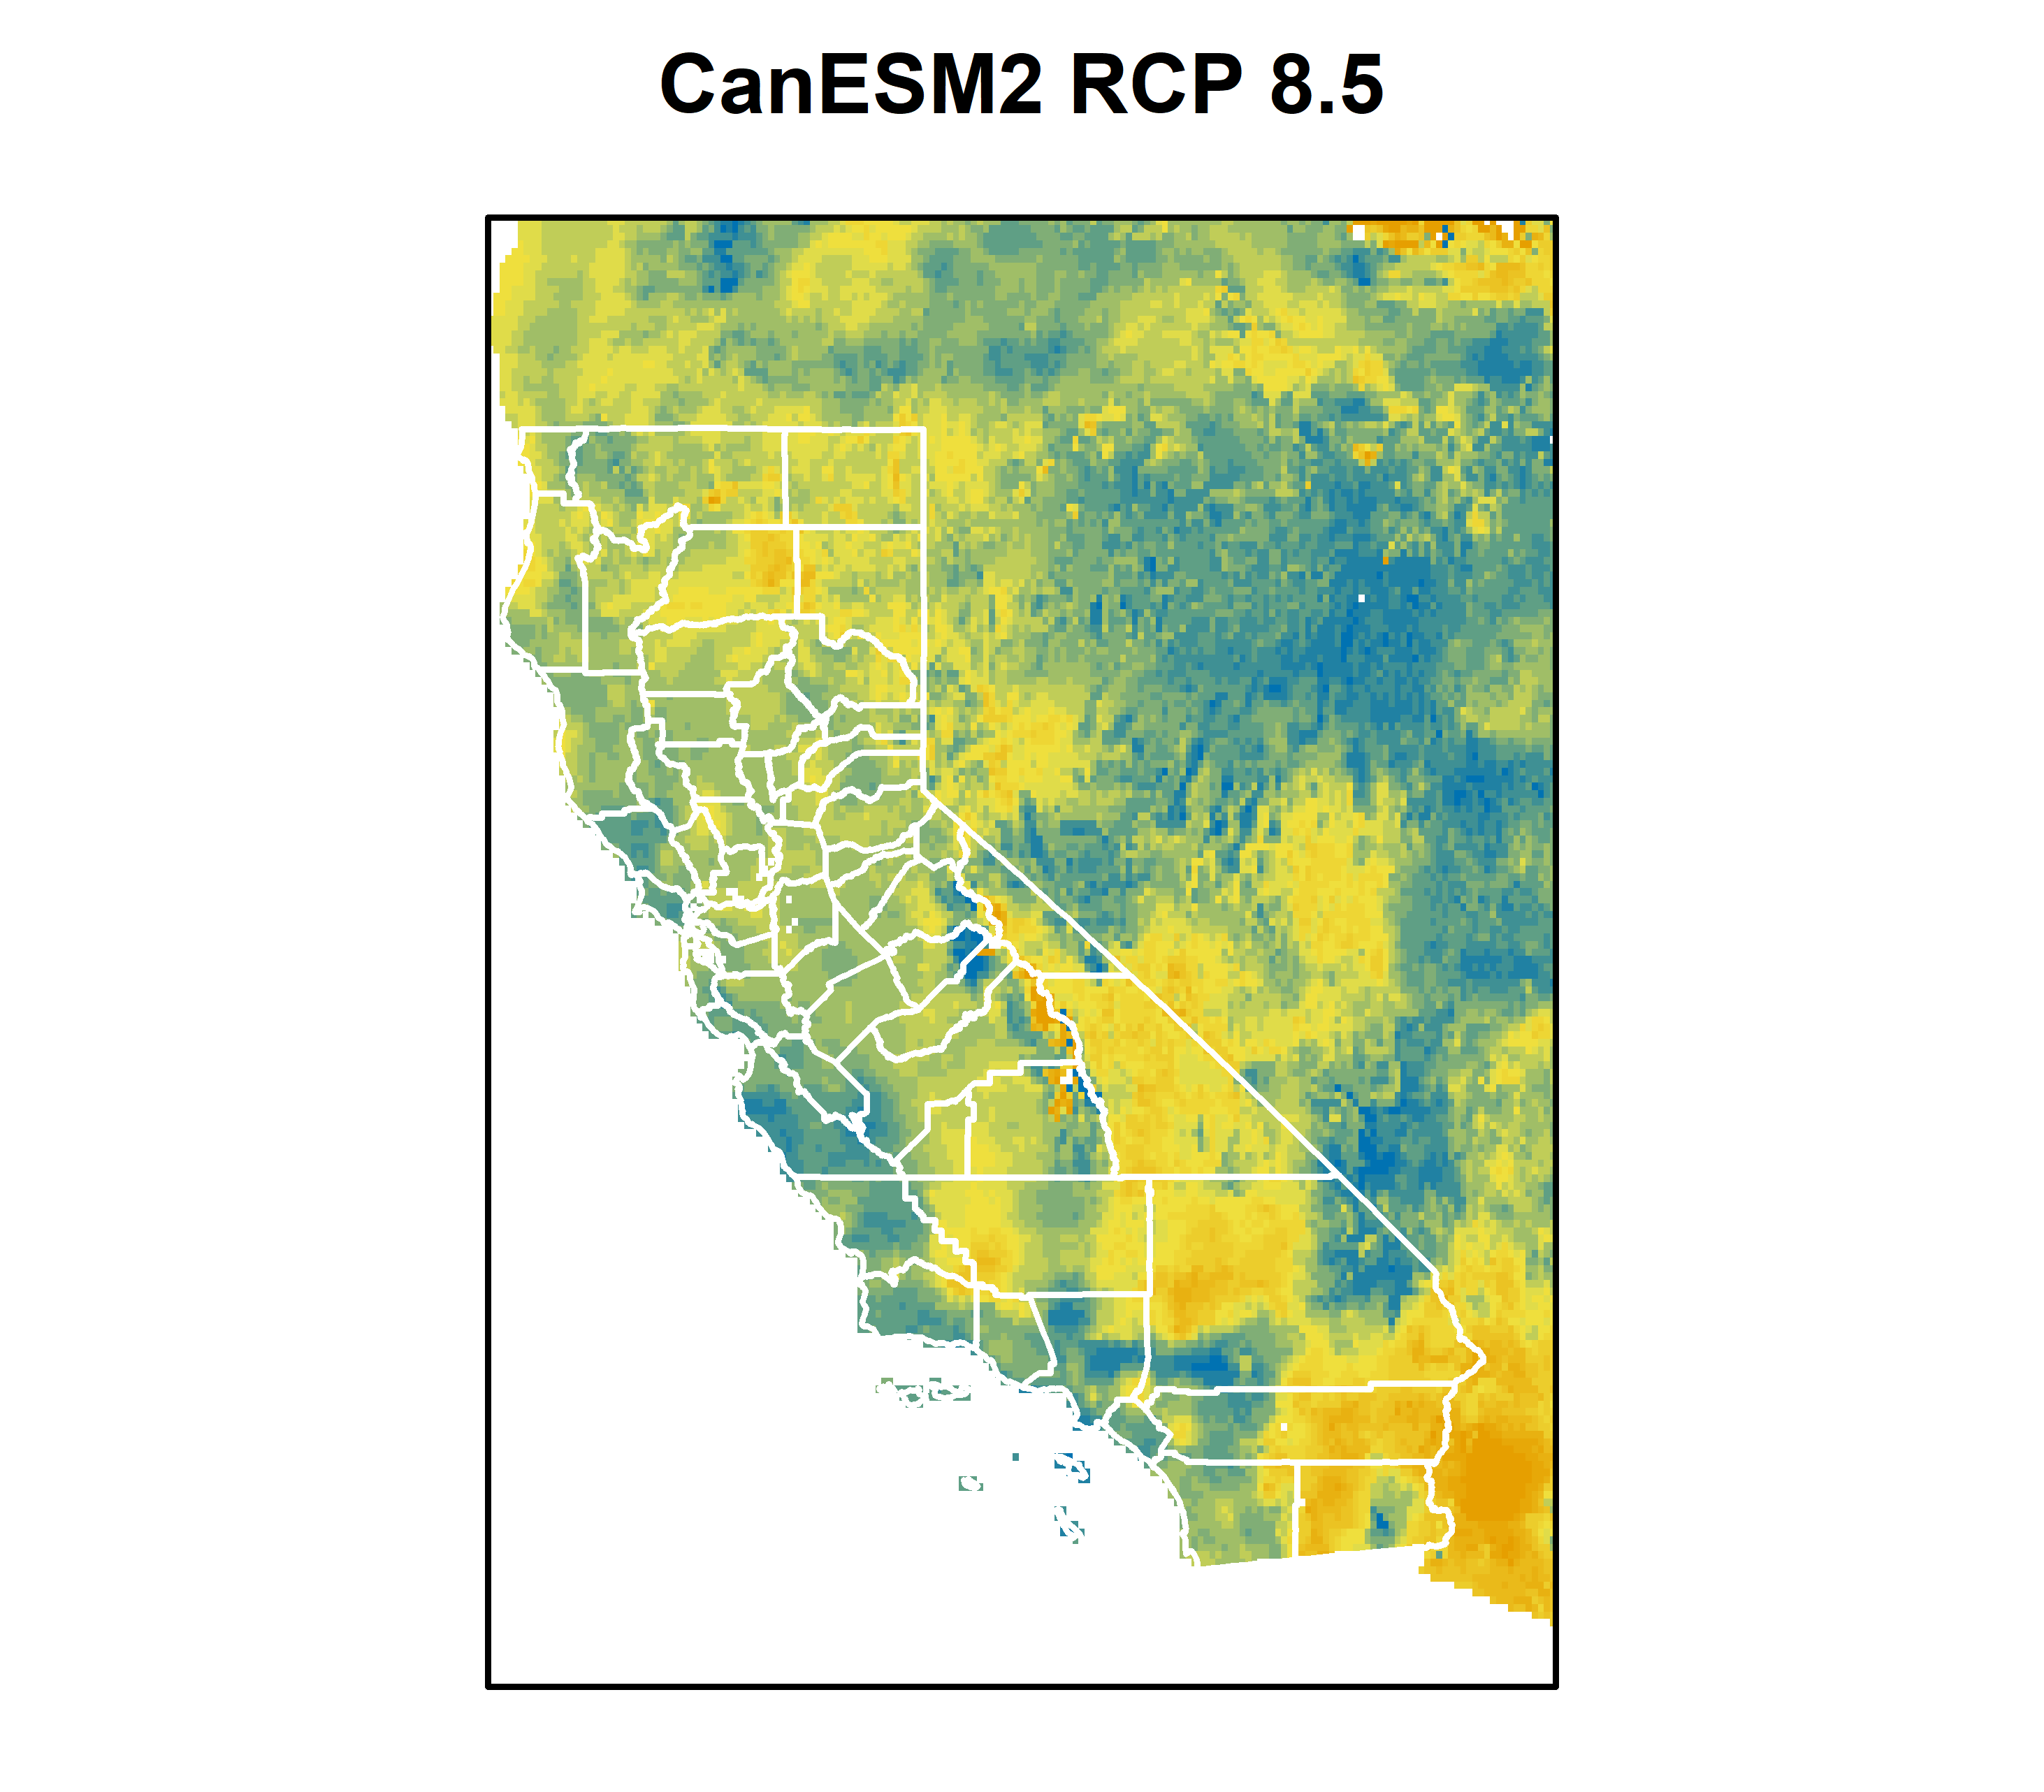
\includegraphics[width=.24\textwidth, trim={1cm 0 0 0}]{plots/rplot54_RNF_CanESM2_85_rpd.png}\hfill
    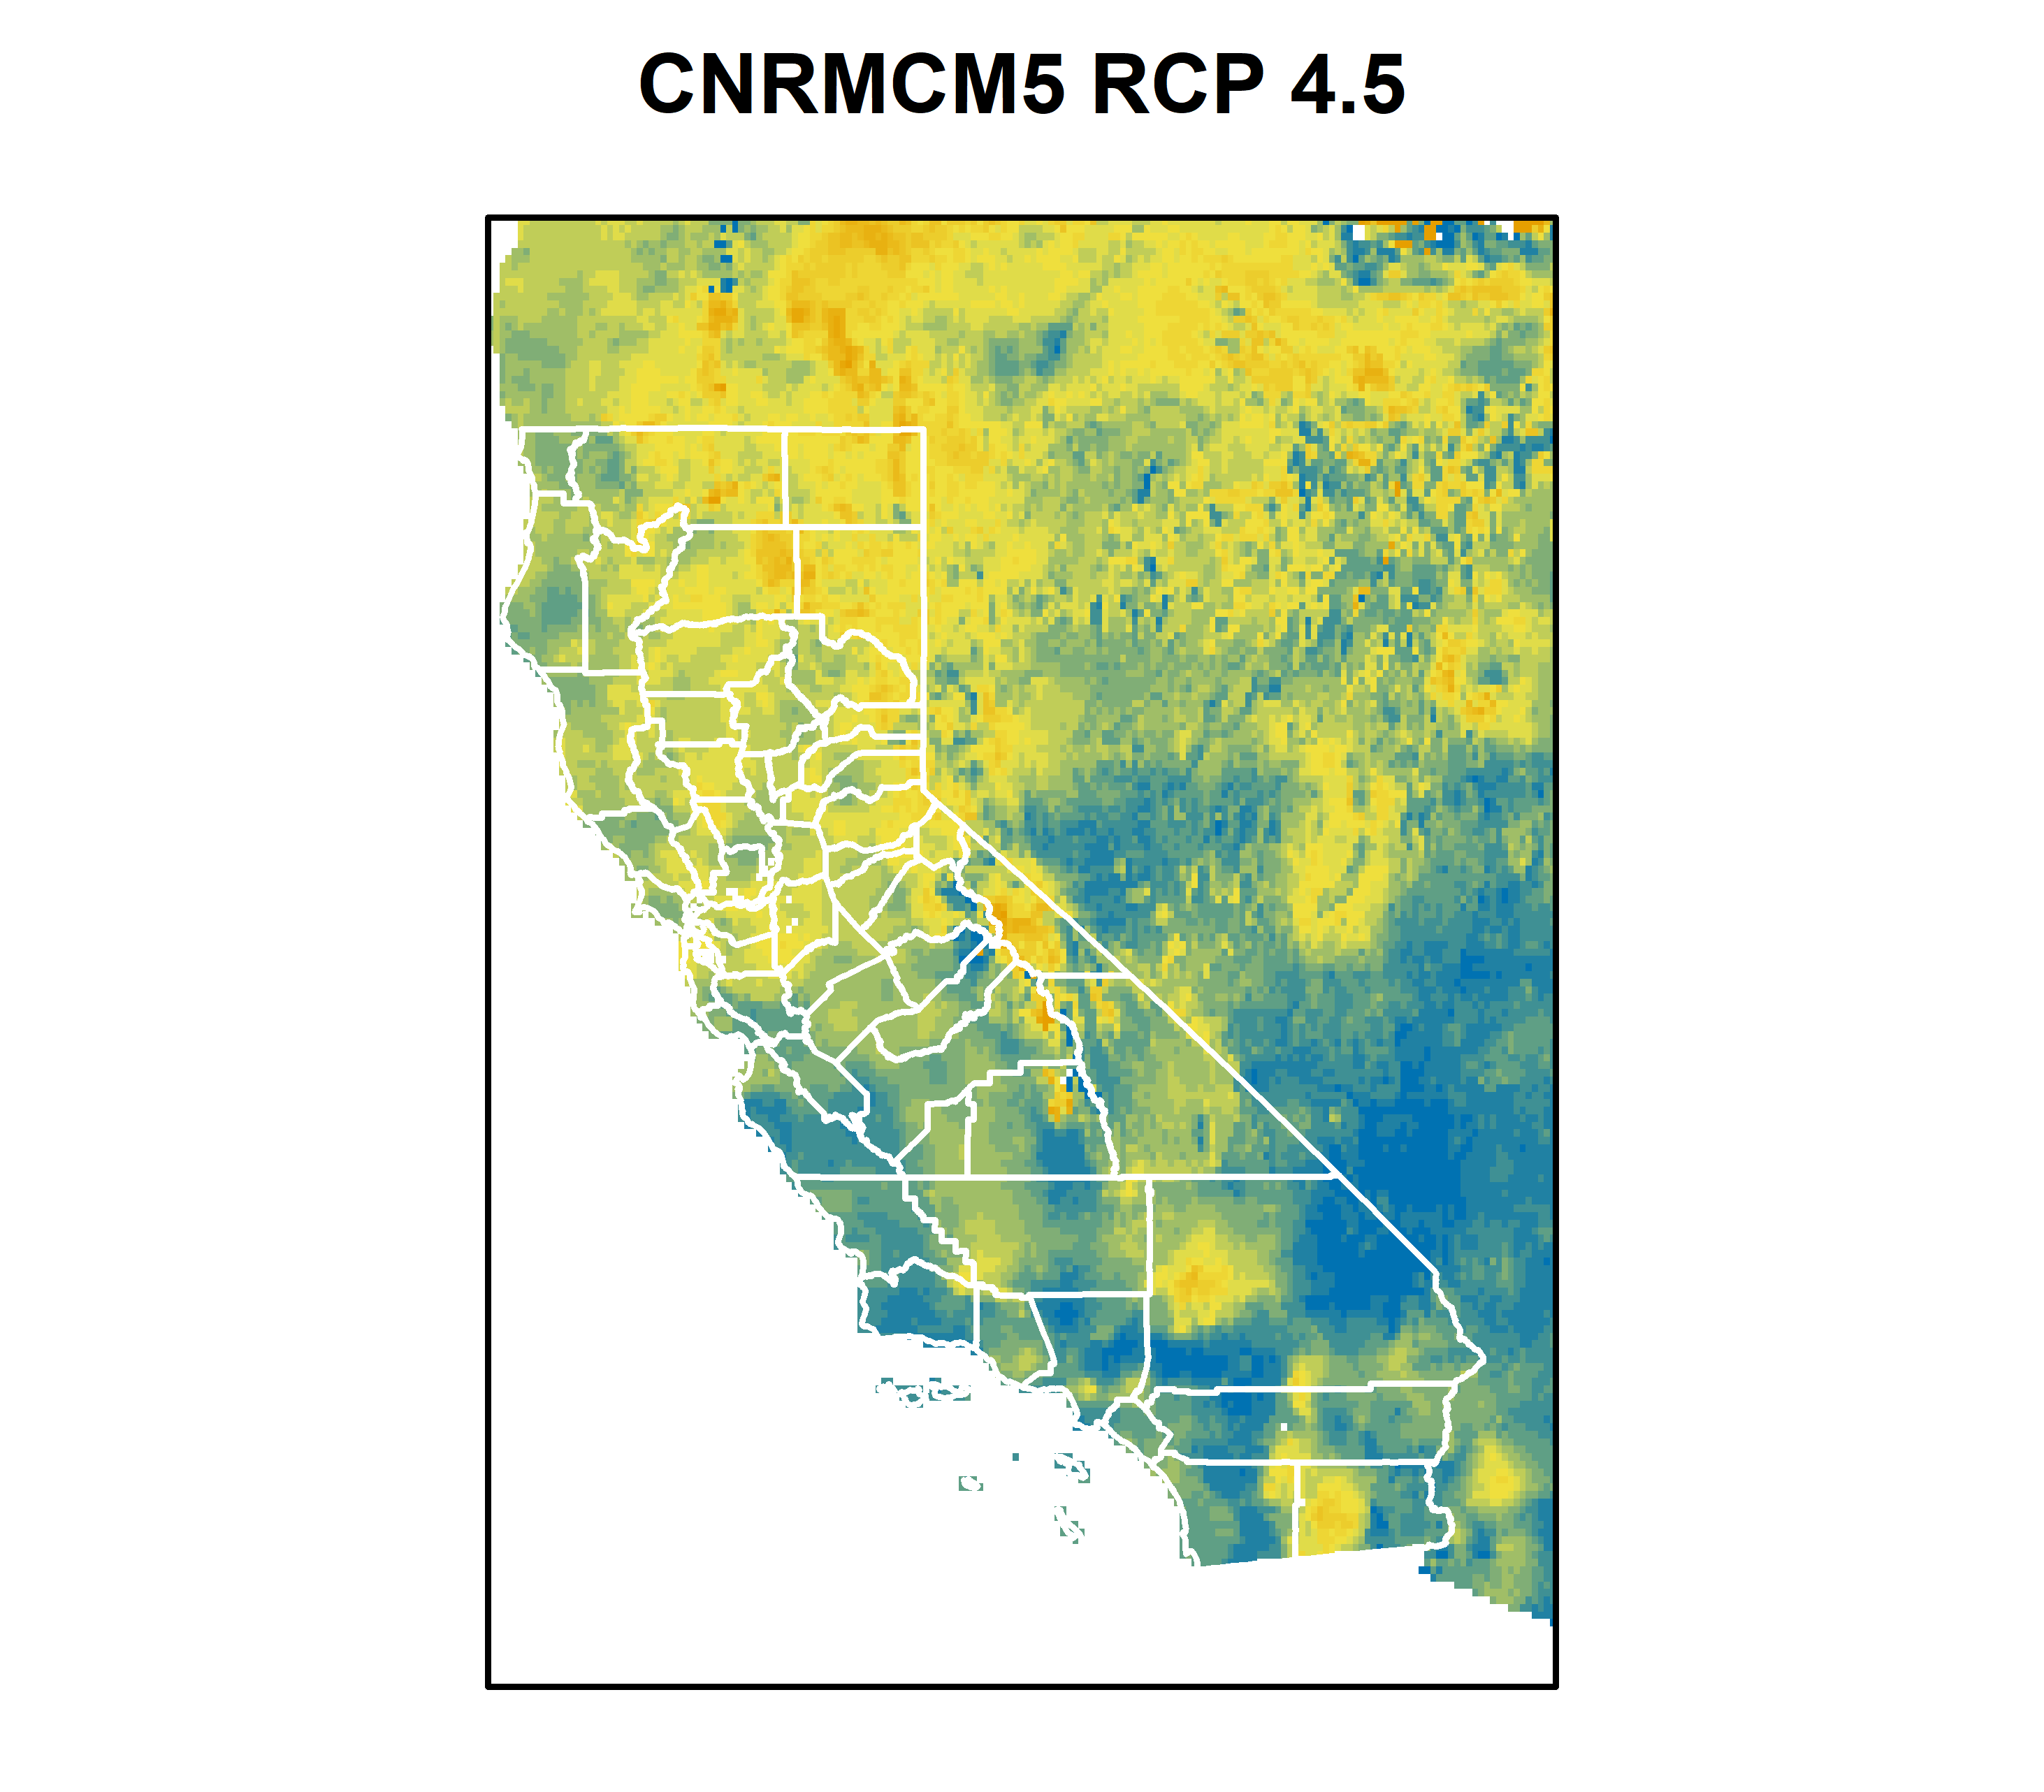
\includegraphics[width=.24\textwidth, trim={1cm 0 0 0}]{plots/rplot54_RNF_CNRMCM5_45_rpd.png}\hfill
    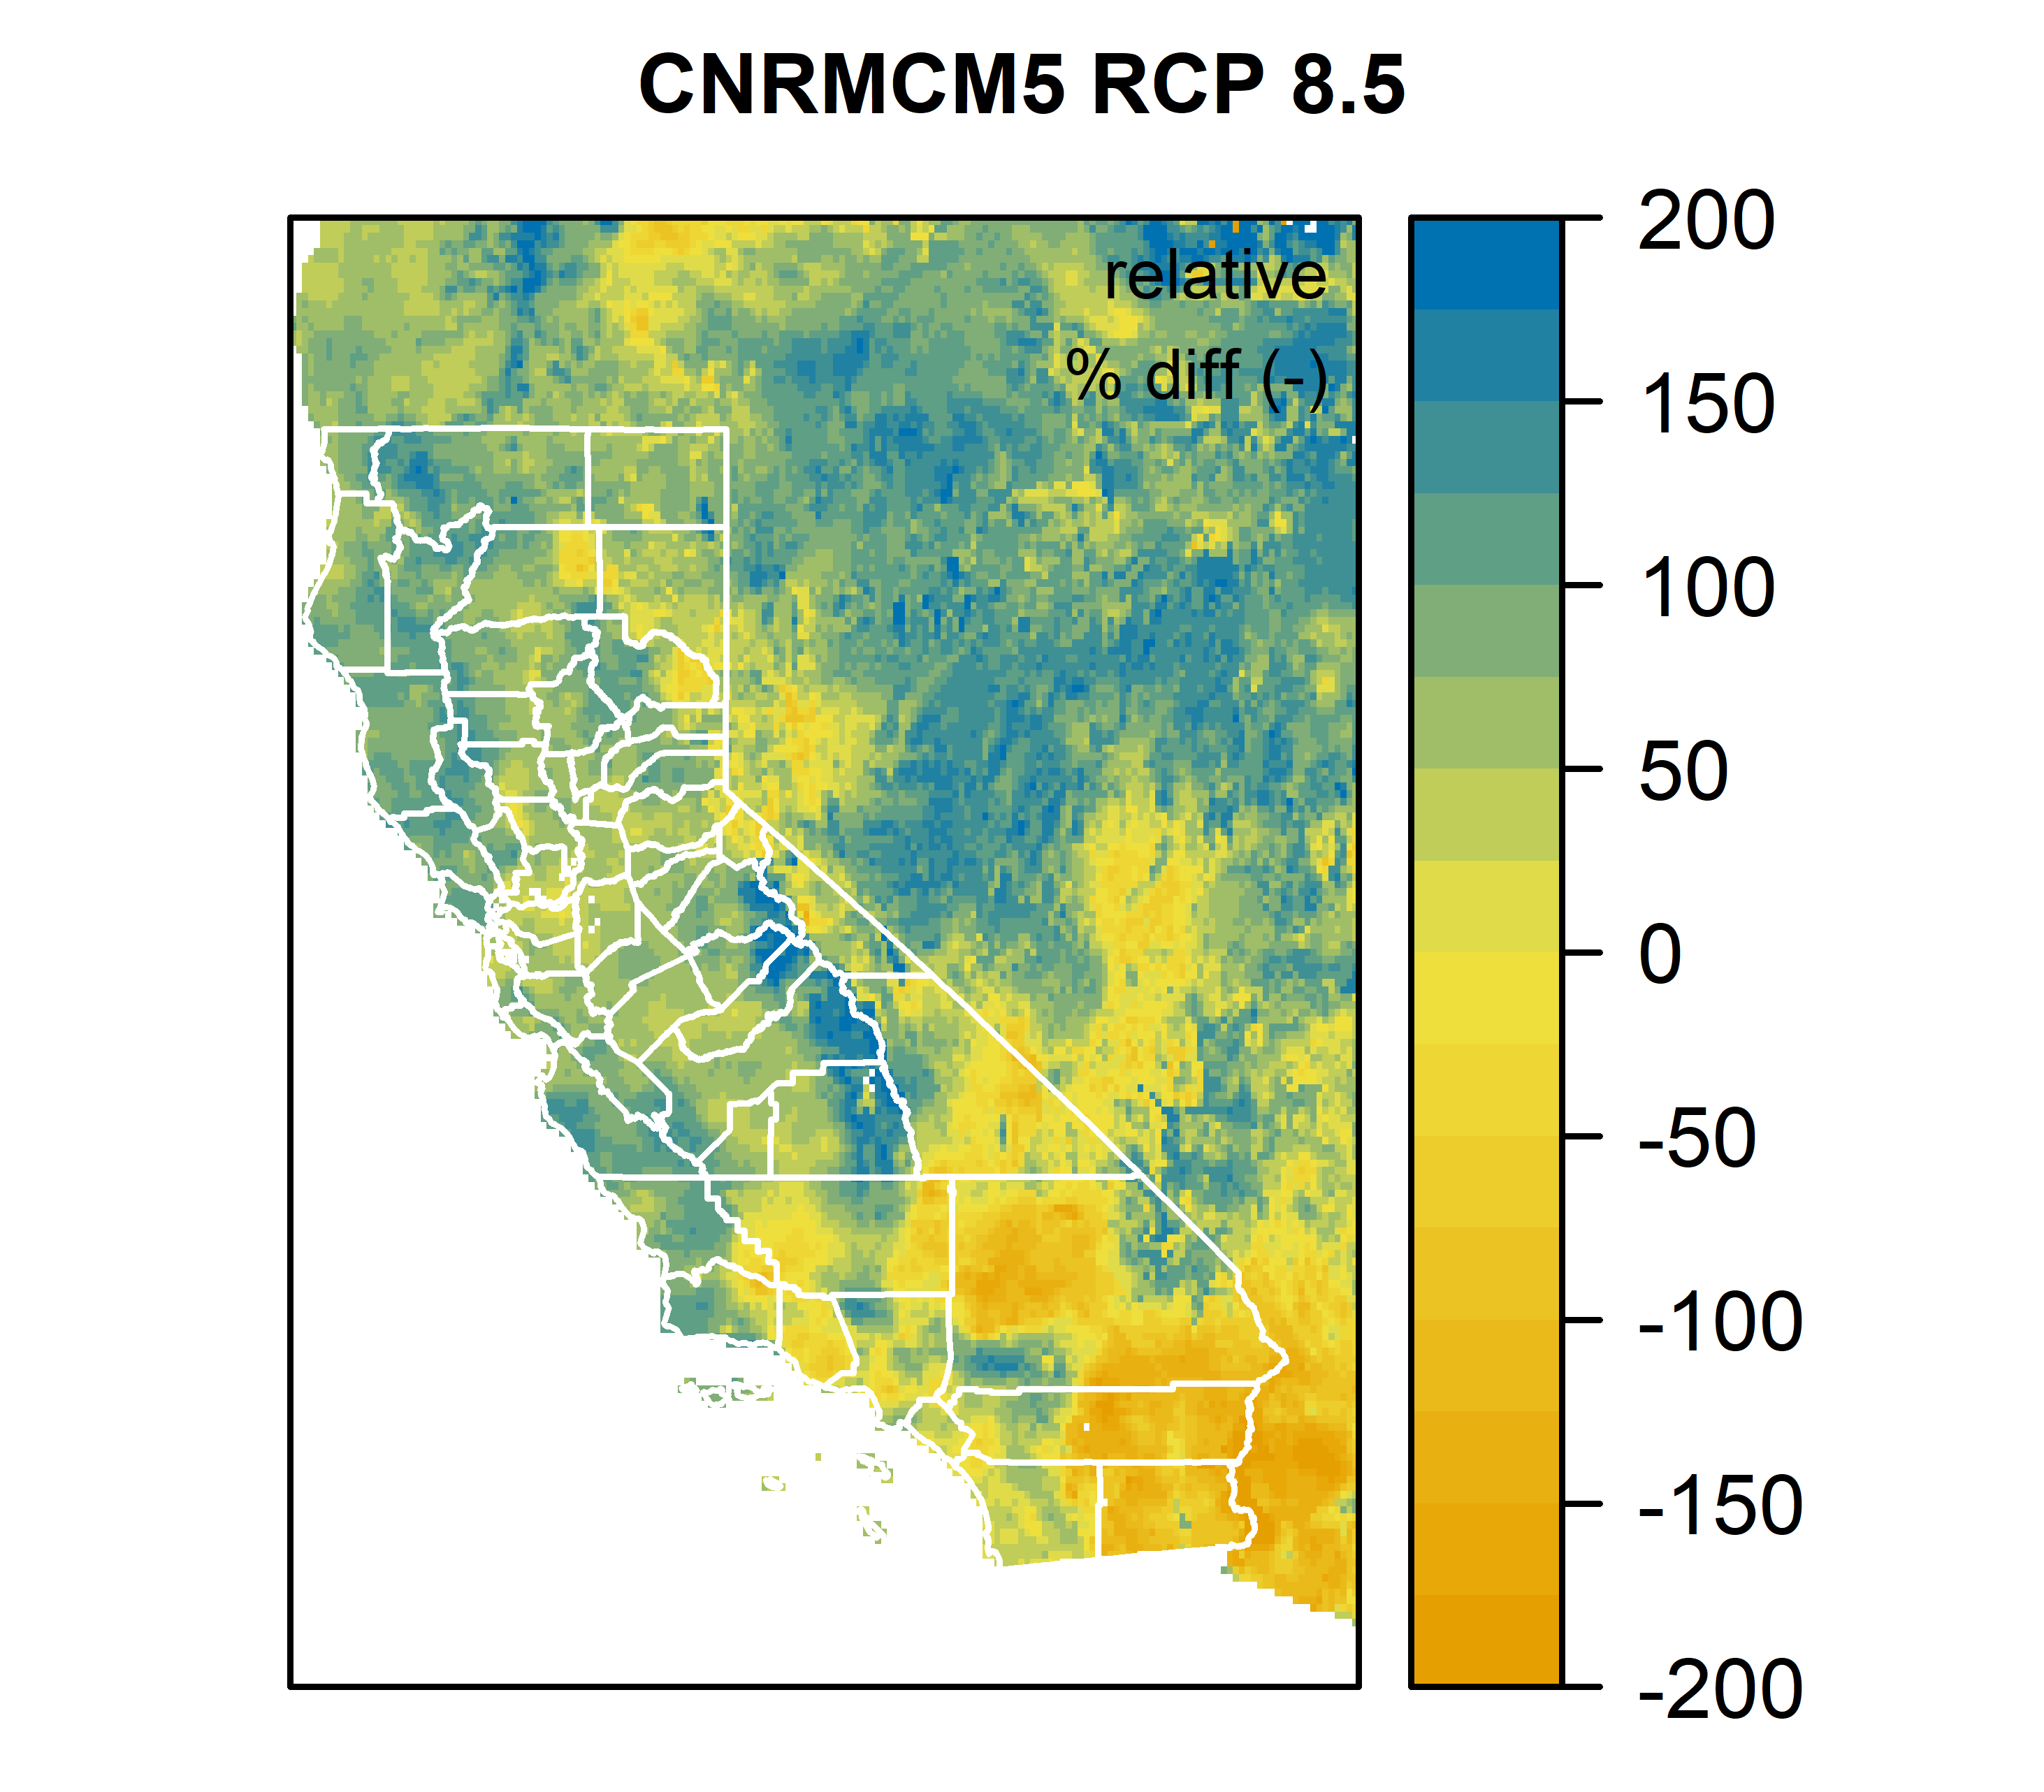
\includegraphics[width=.24\textwidth, trim={1cm 0 0 0}]{plots/rplot54_RNF_CNRMCM5_85_rpd.png}
    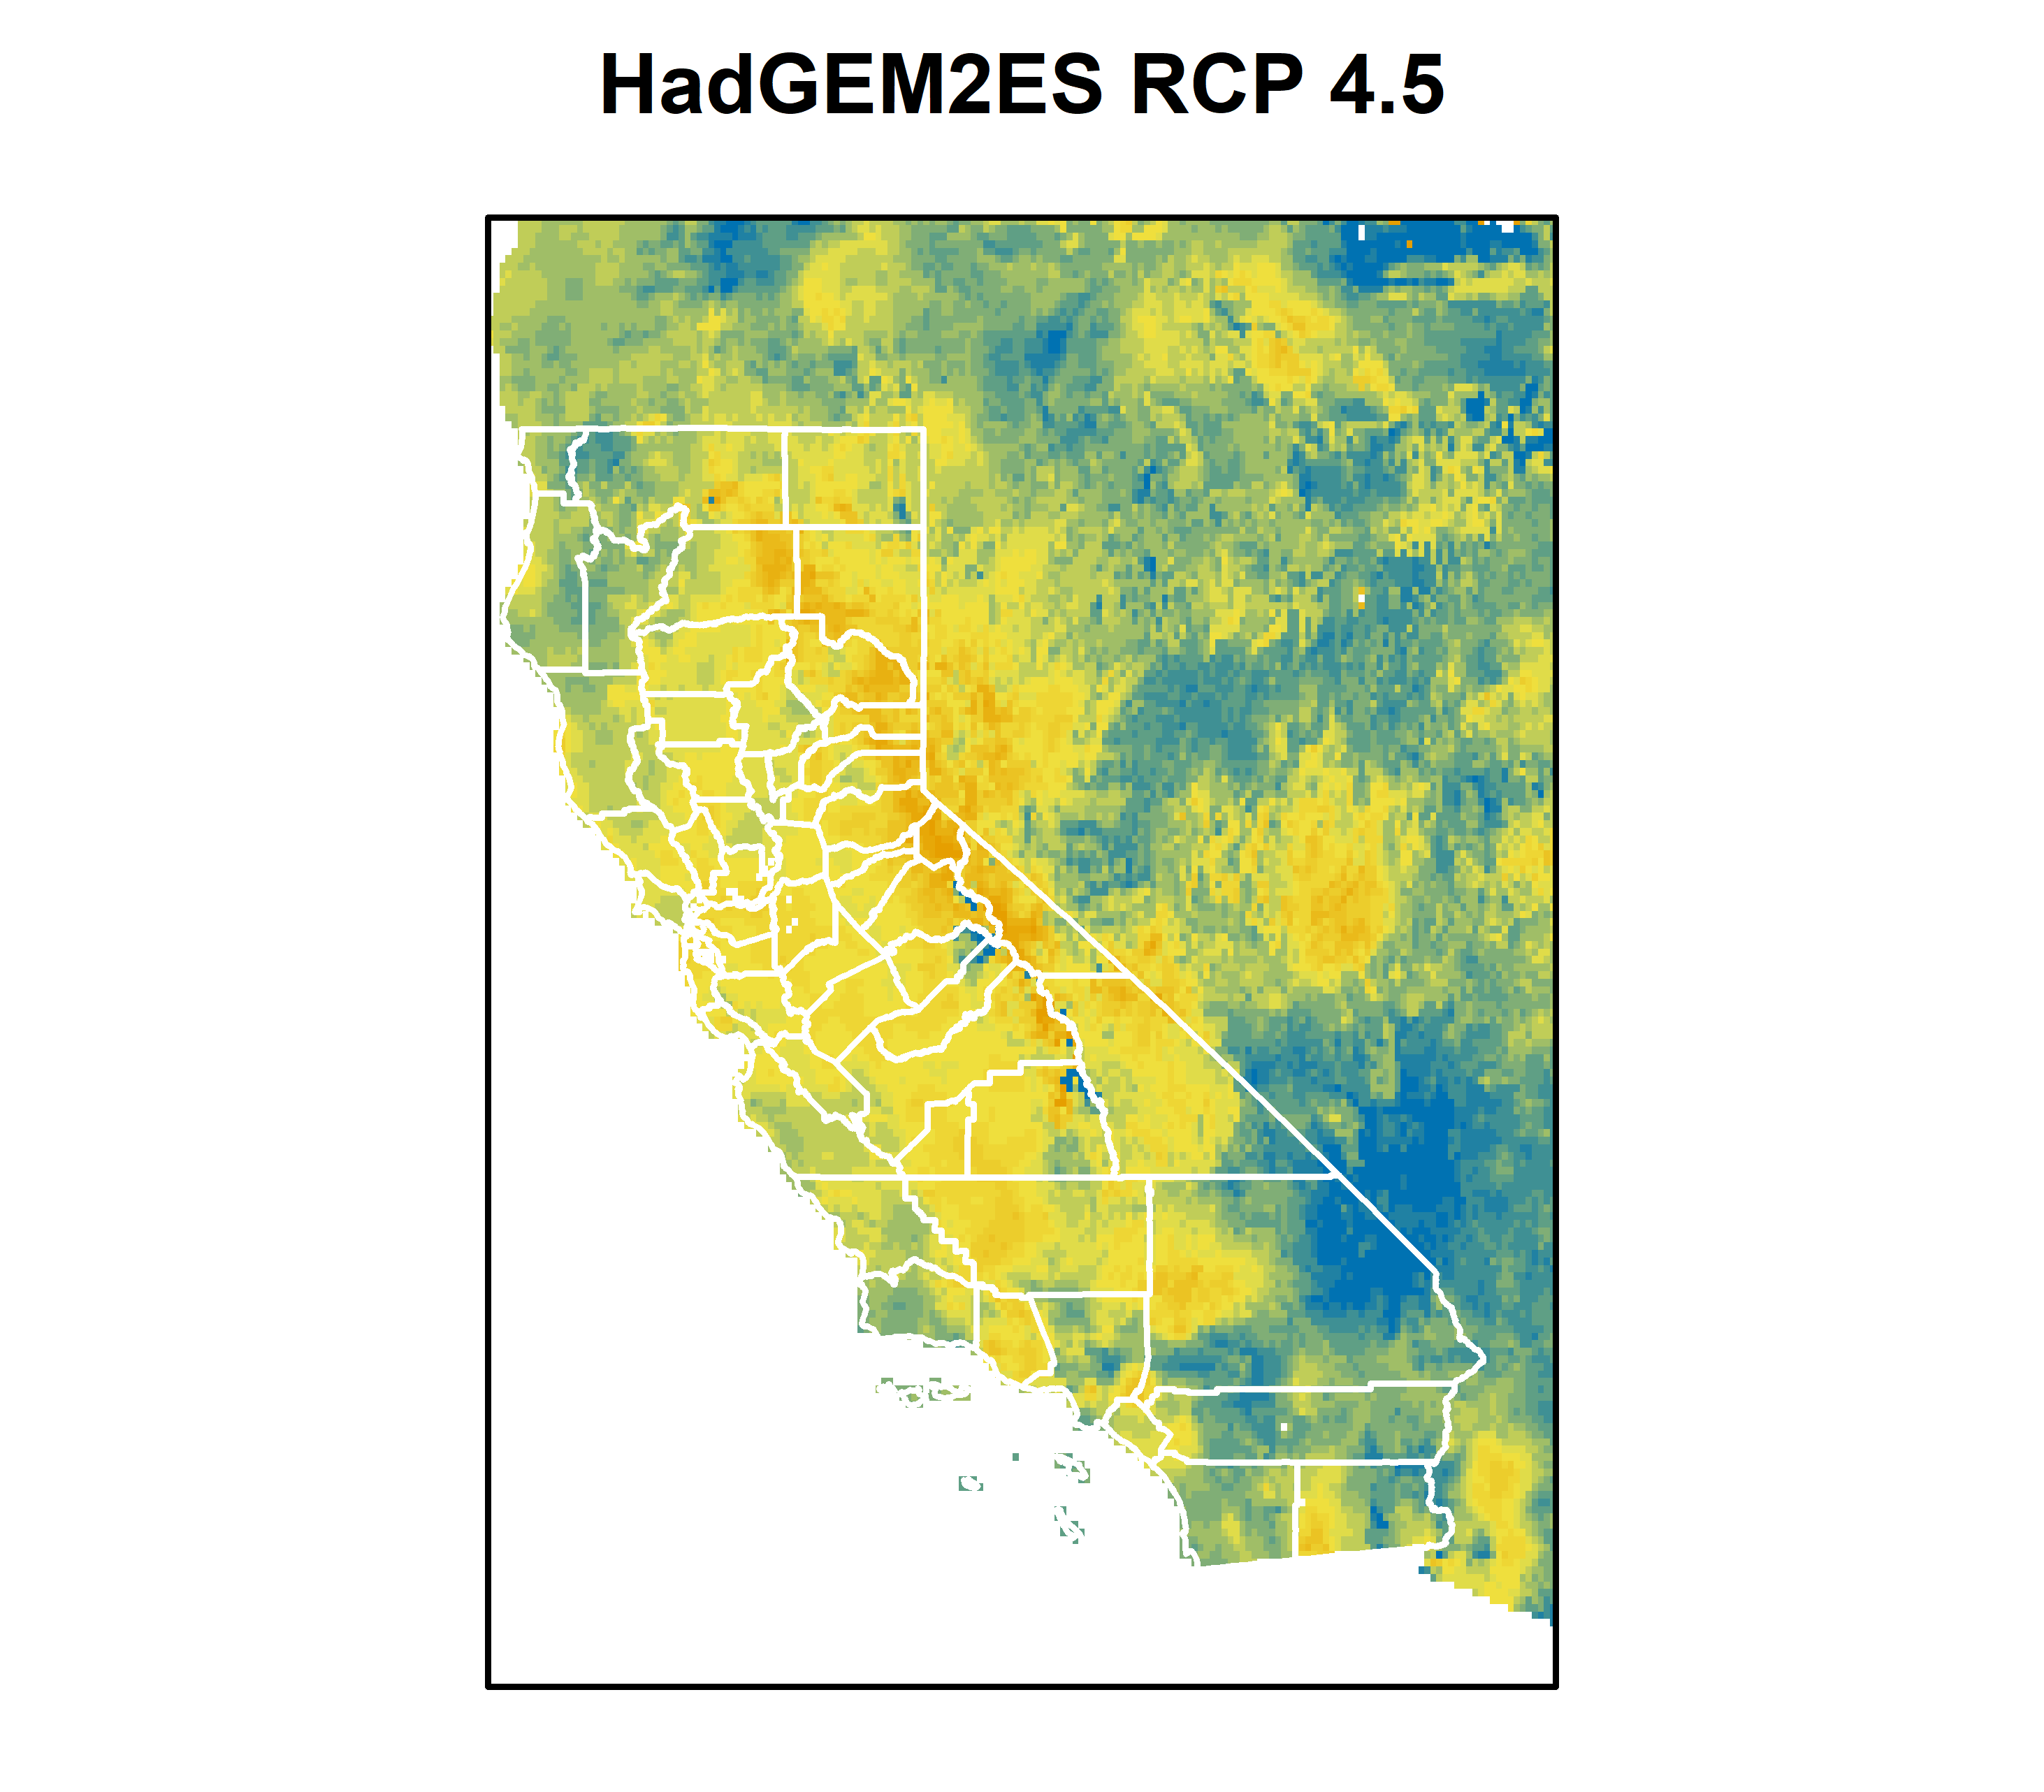
\includegraphics[width=.24\textwidth, trim={1cm 0 0 0}]{plots/rplot54_RNF_HadGEM2ES_45_rpd.png}\hfill
    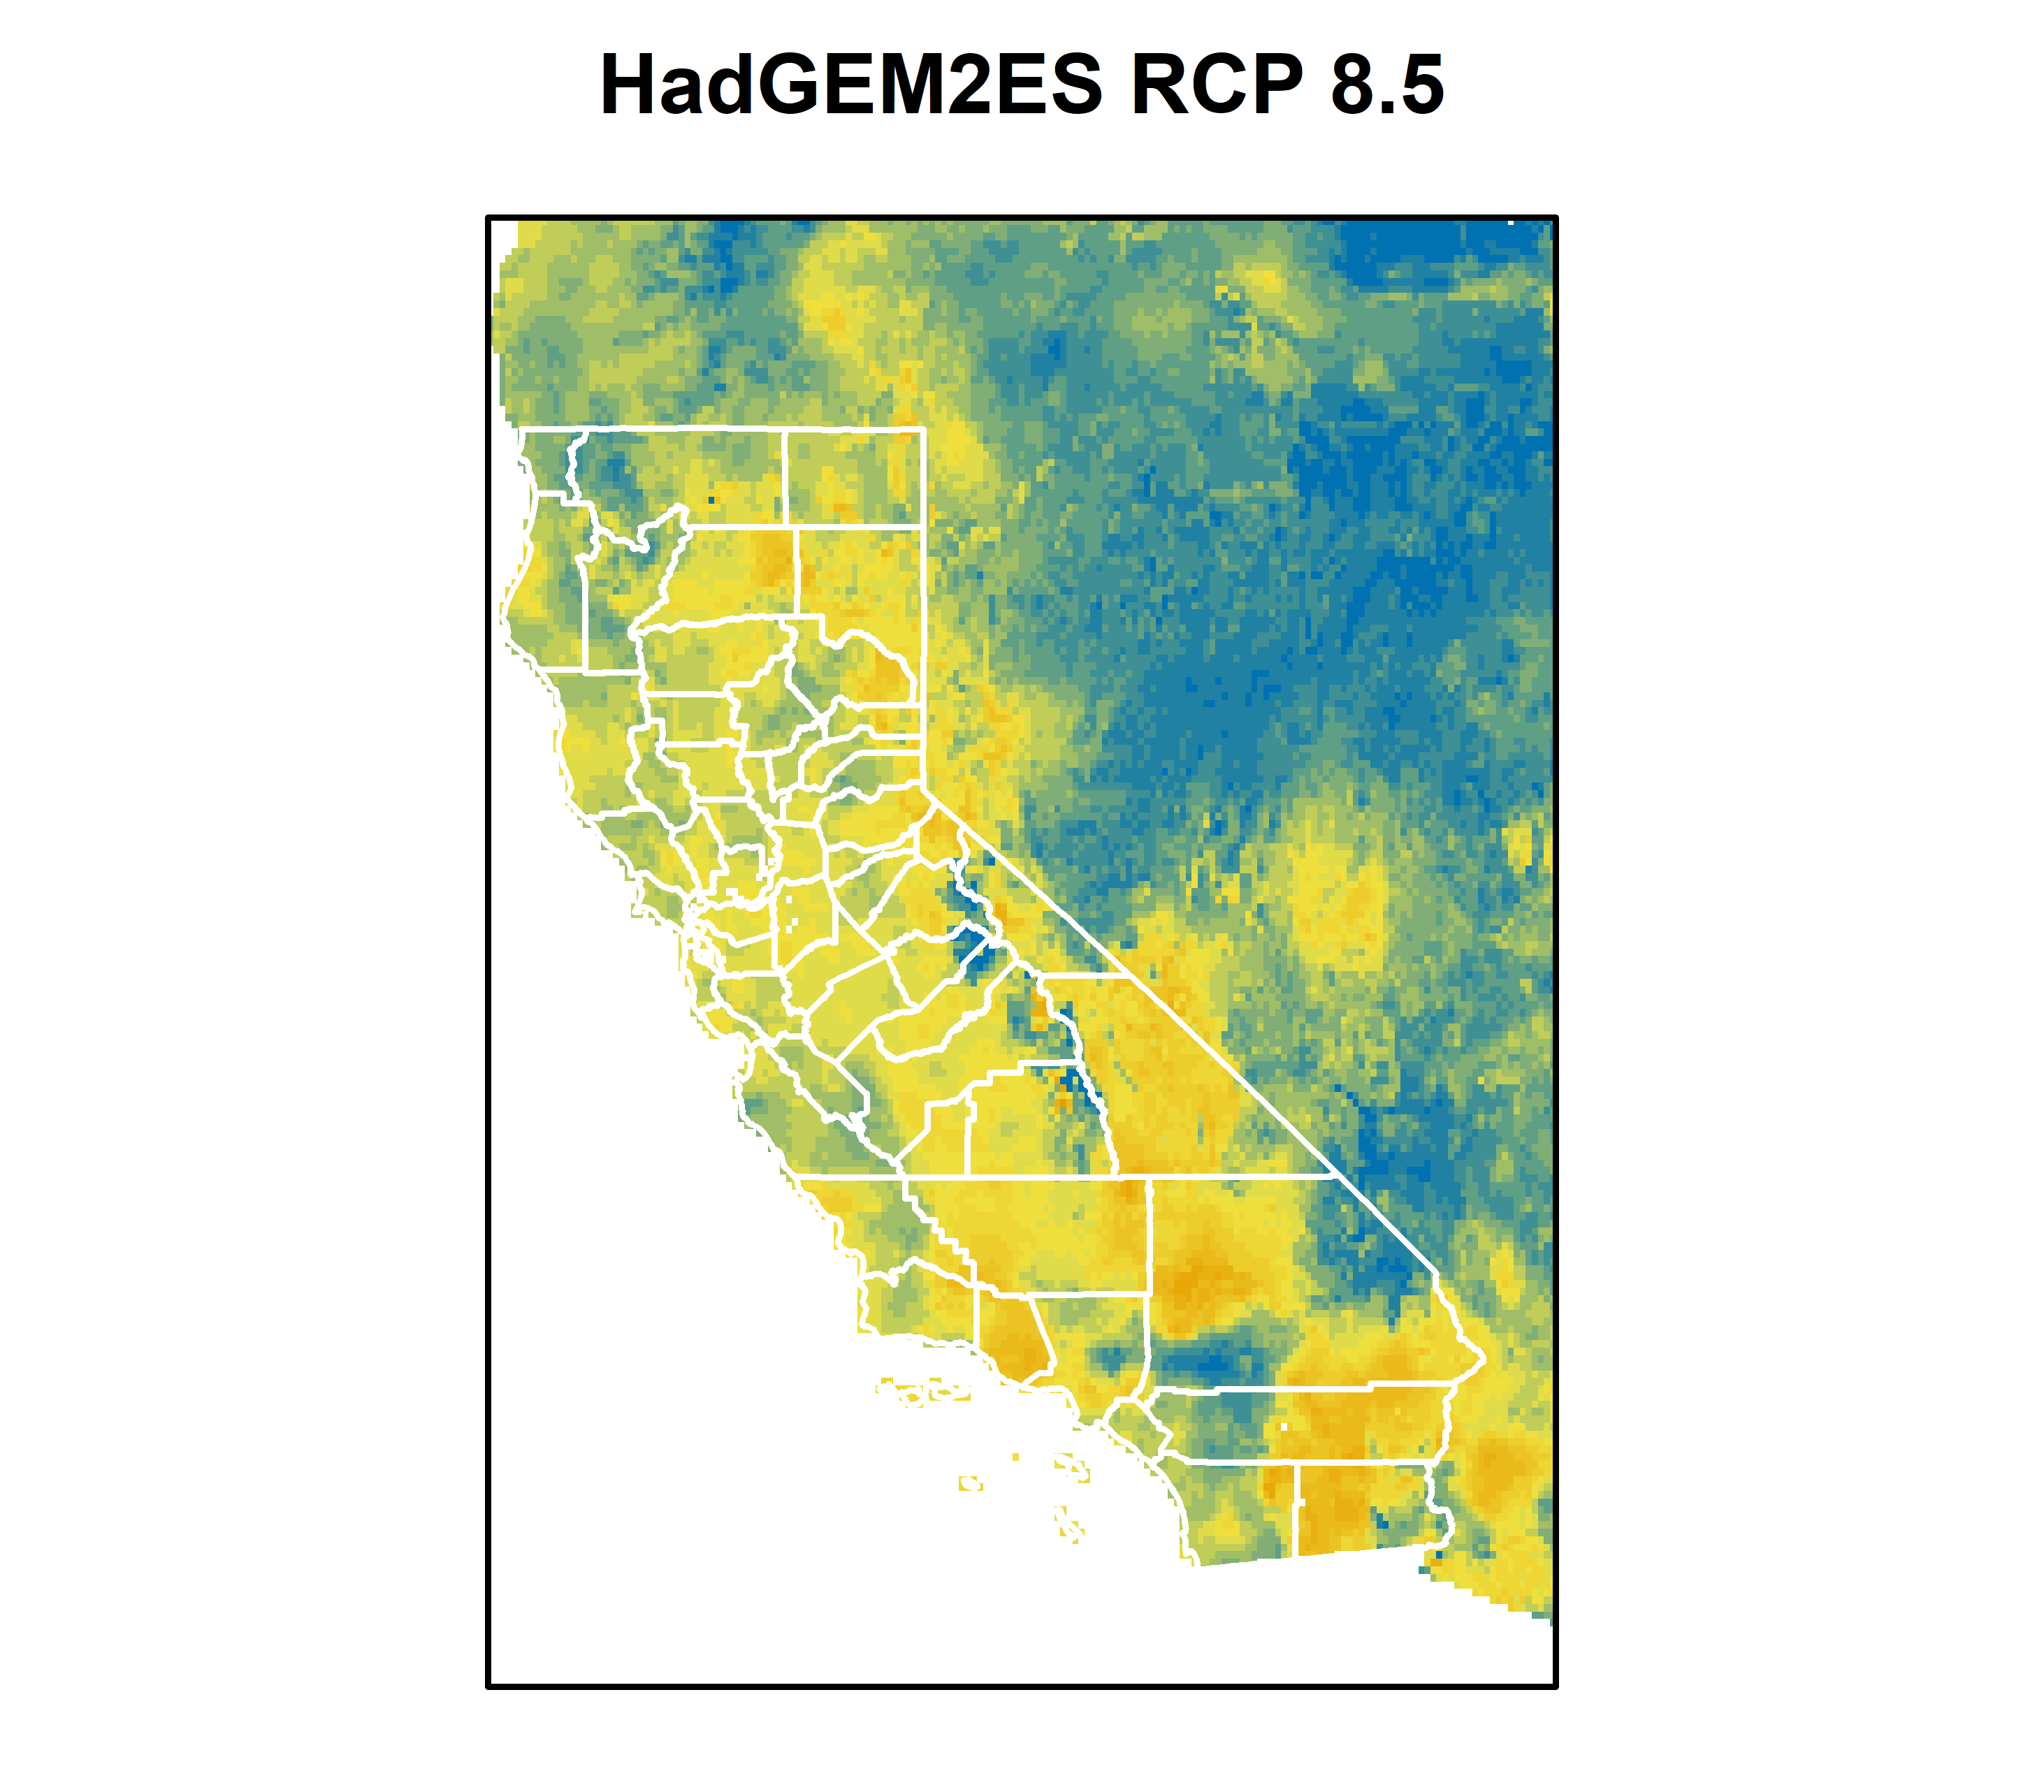
\includegraphics[width=.24\textwidth, trim={1cm 0 0 0}]{plots/rplot54_RNF_HadGEM2ES_85_rpd.png}\hfill
    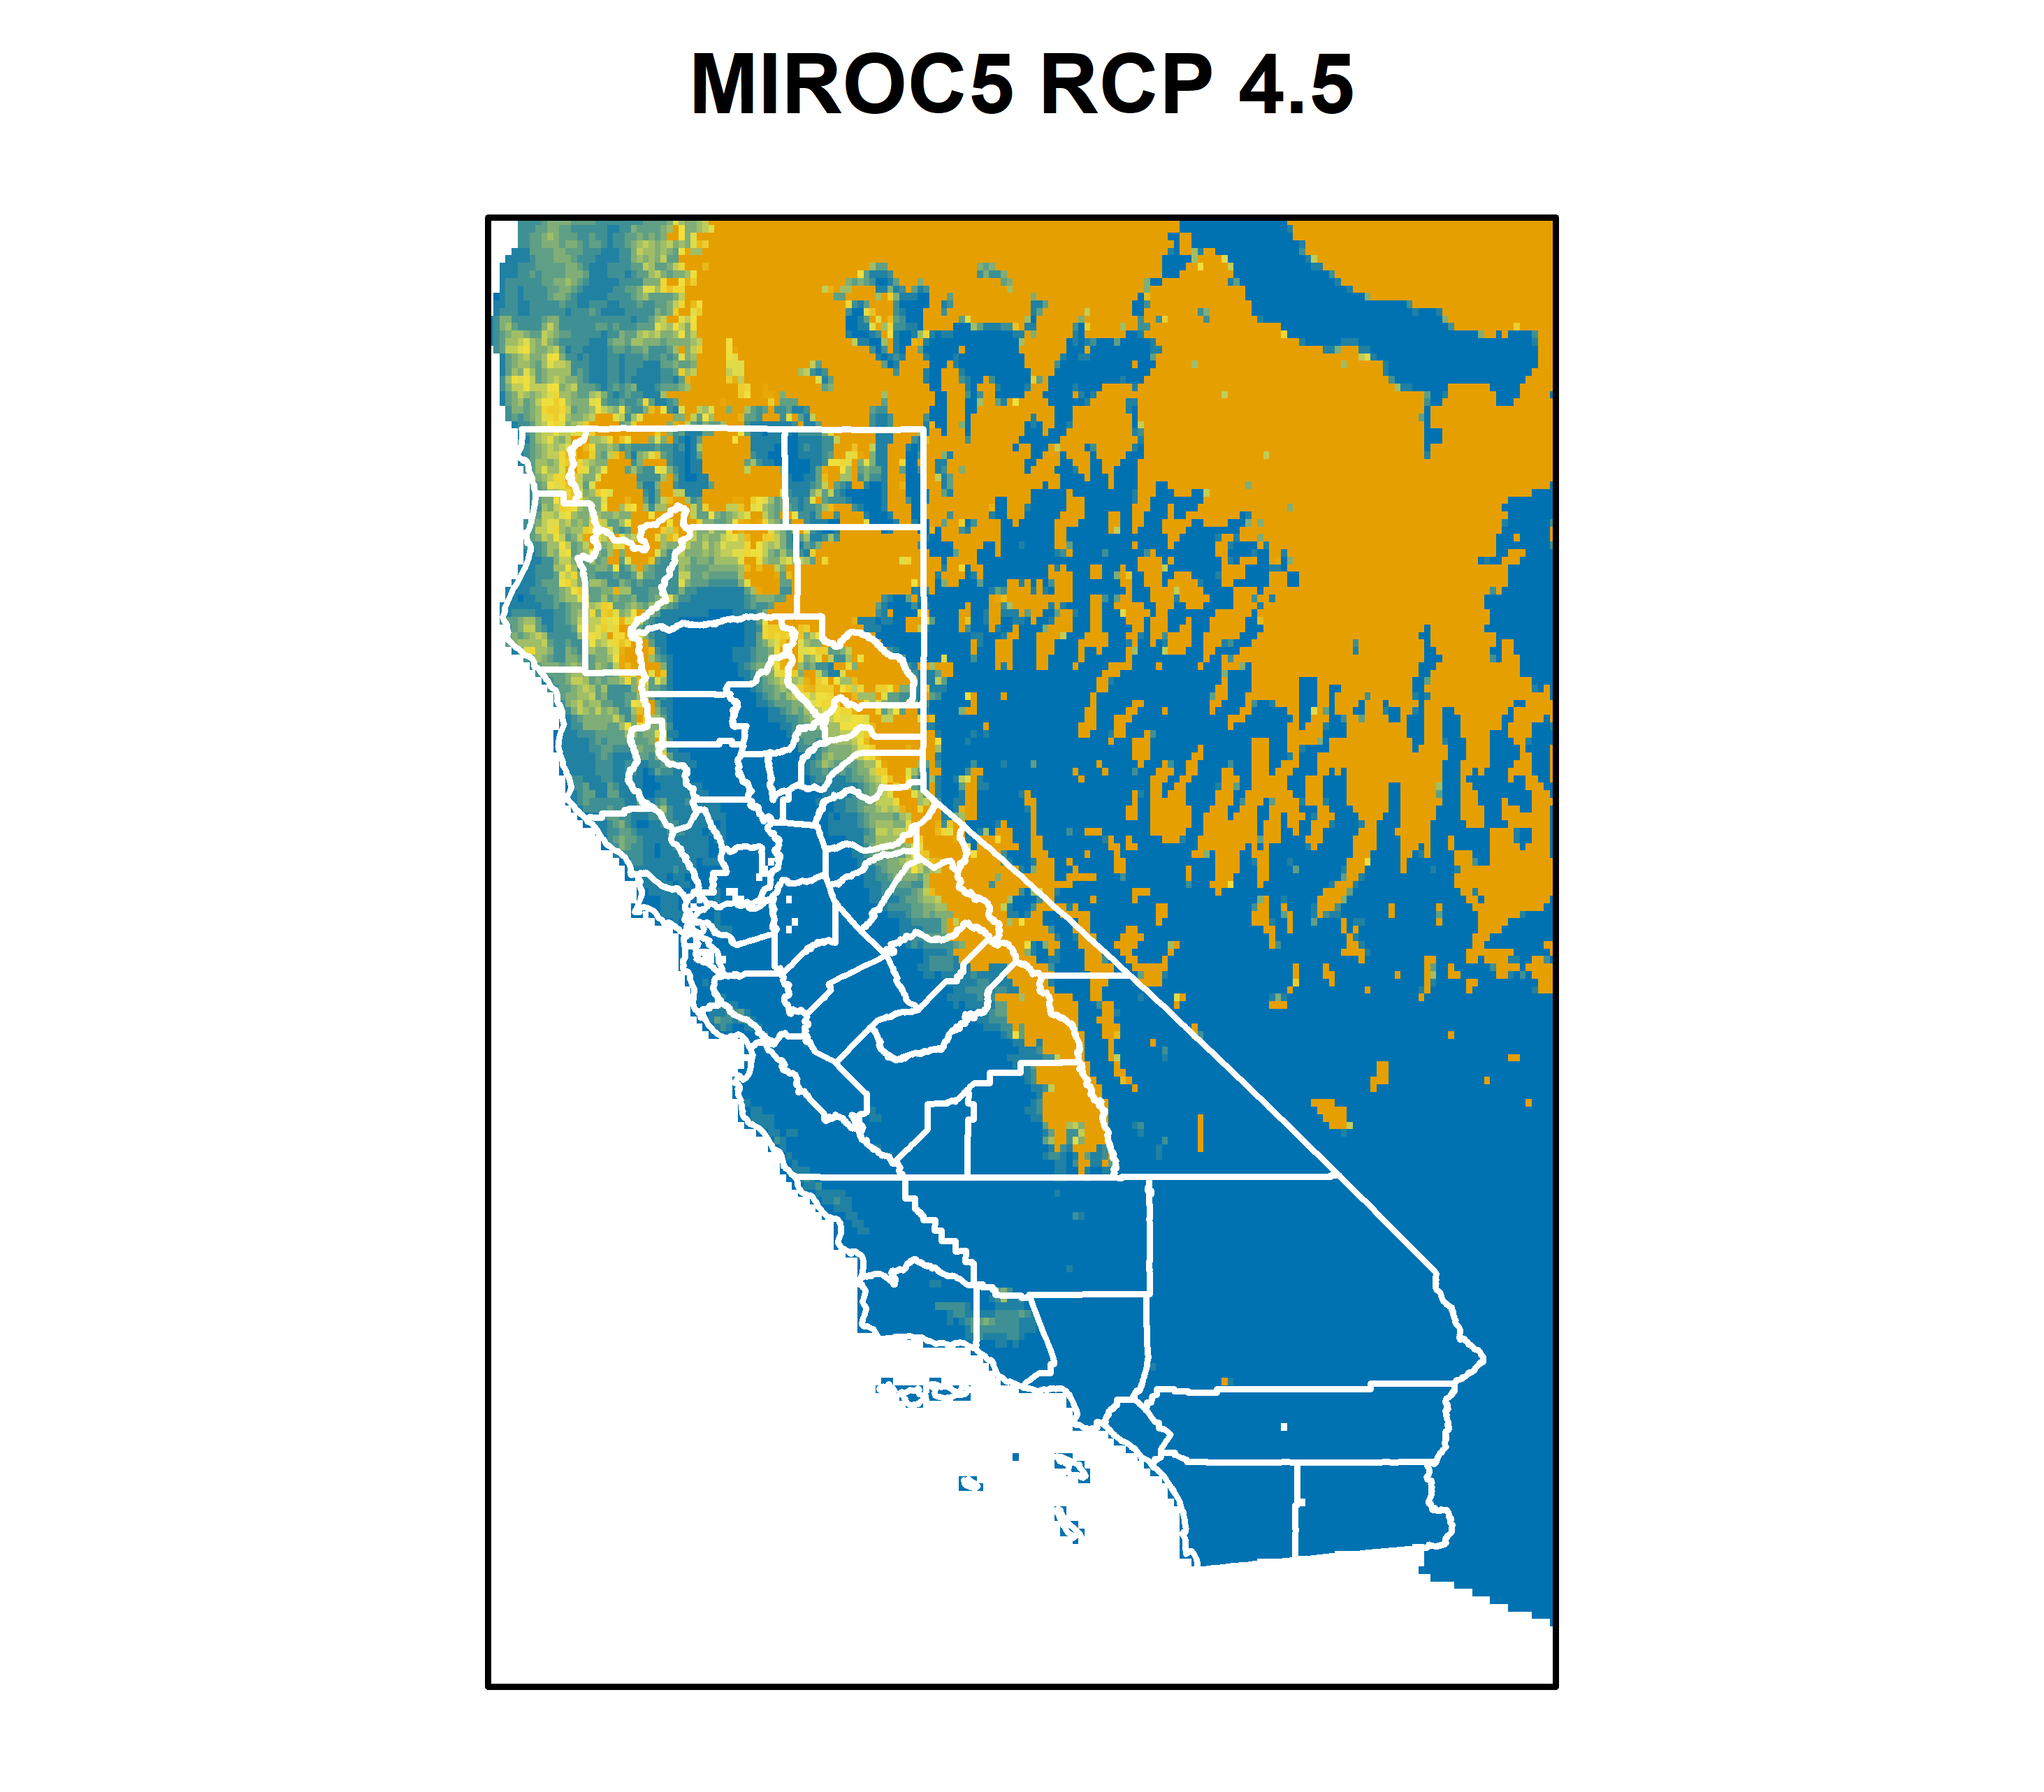
\includegraphics[width=.24\textwidth, trim={1cm 0 0 0}]{plots/rplot54_RNF_MIROC5_45_rpd.png}\hfill
    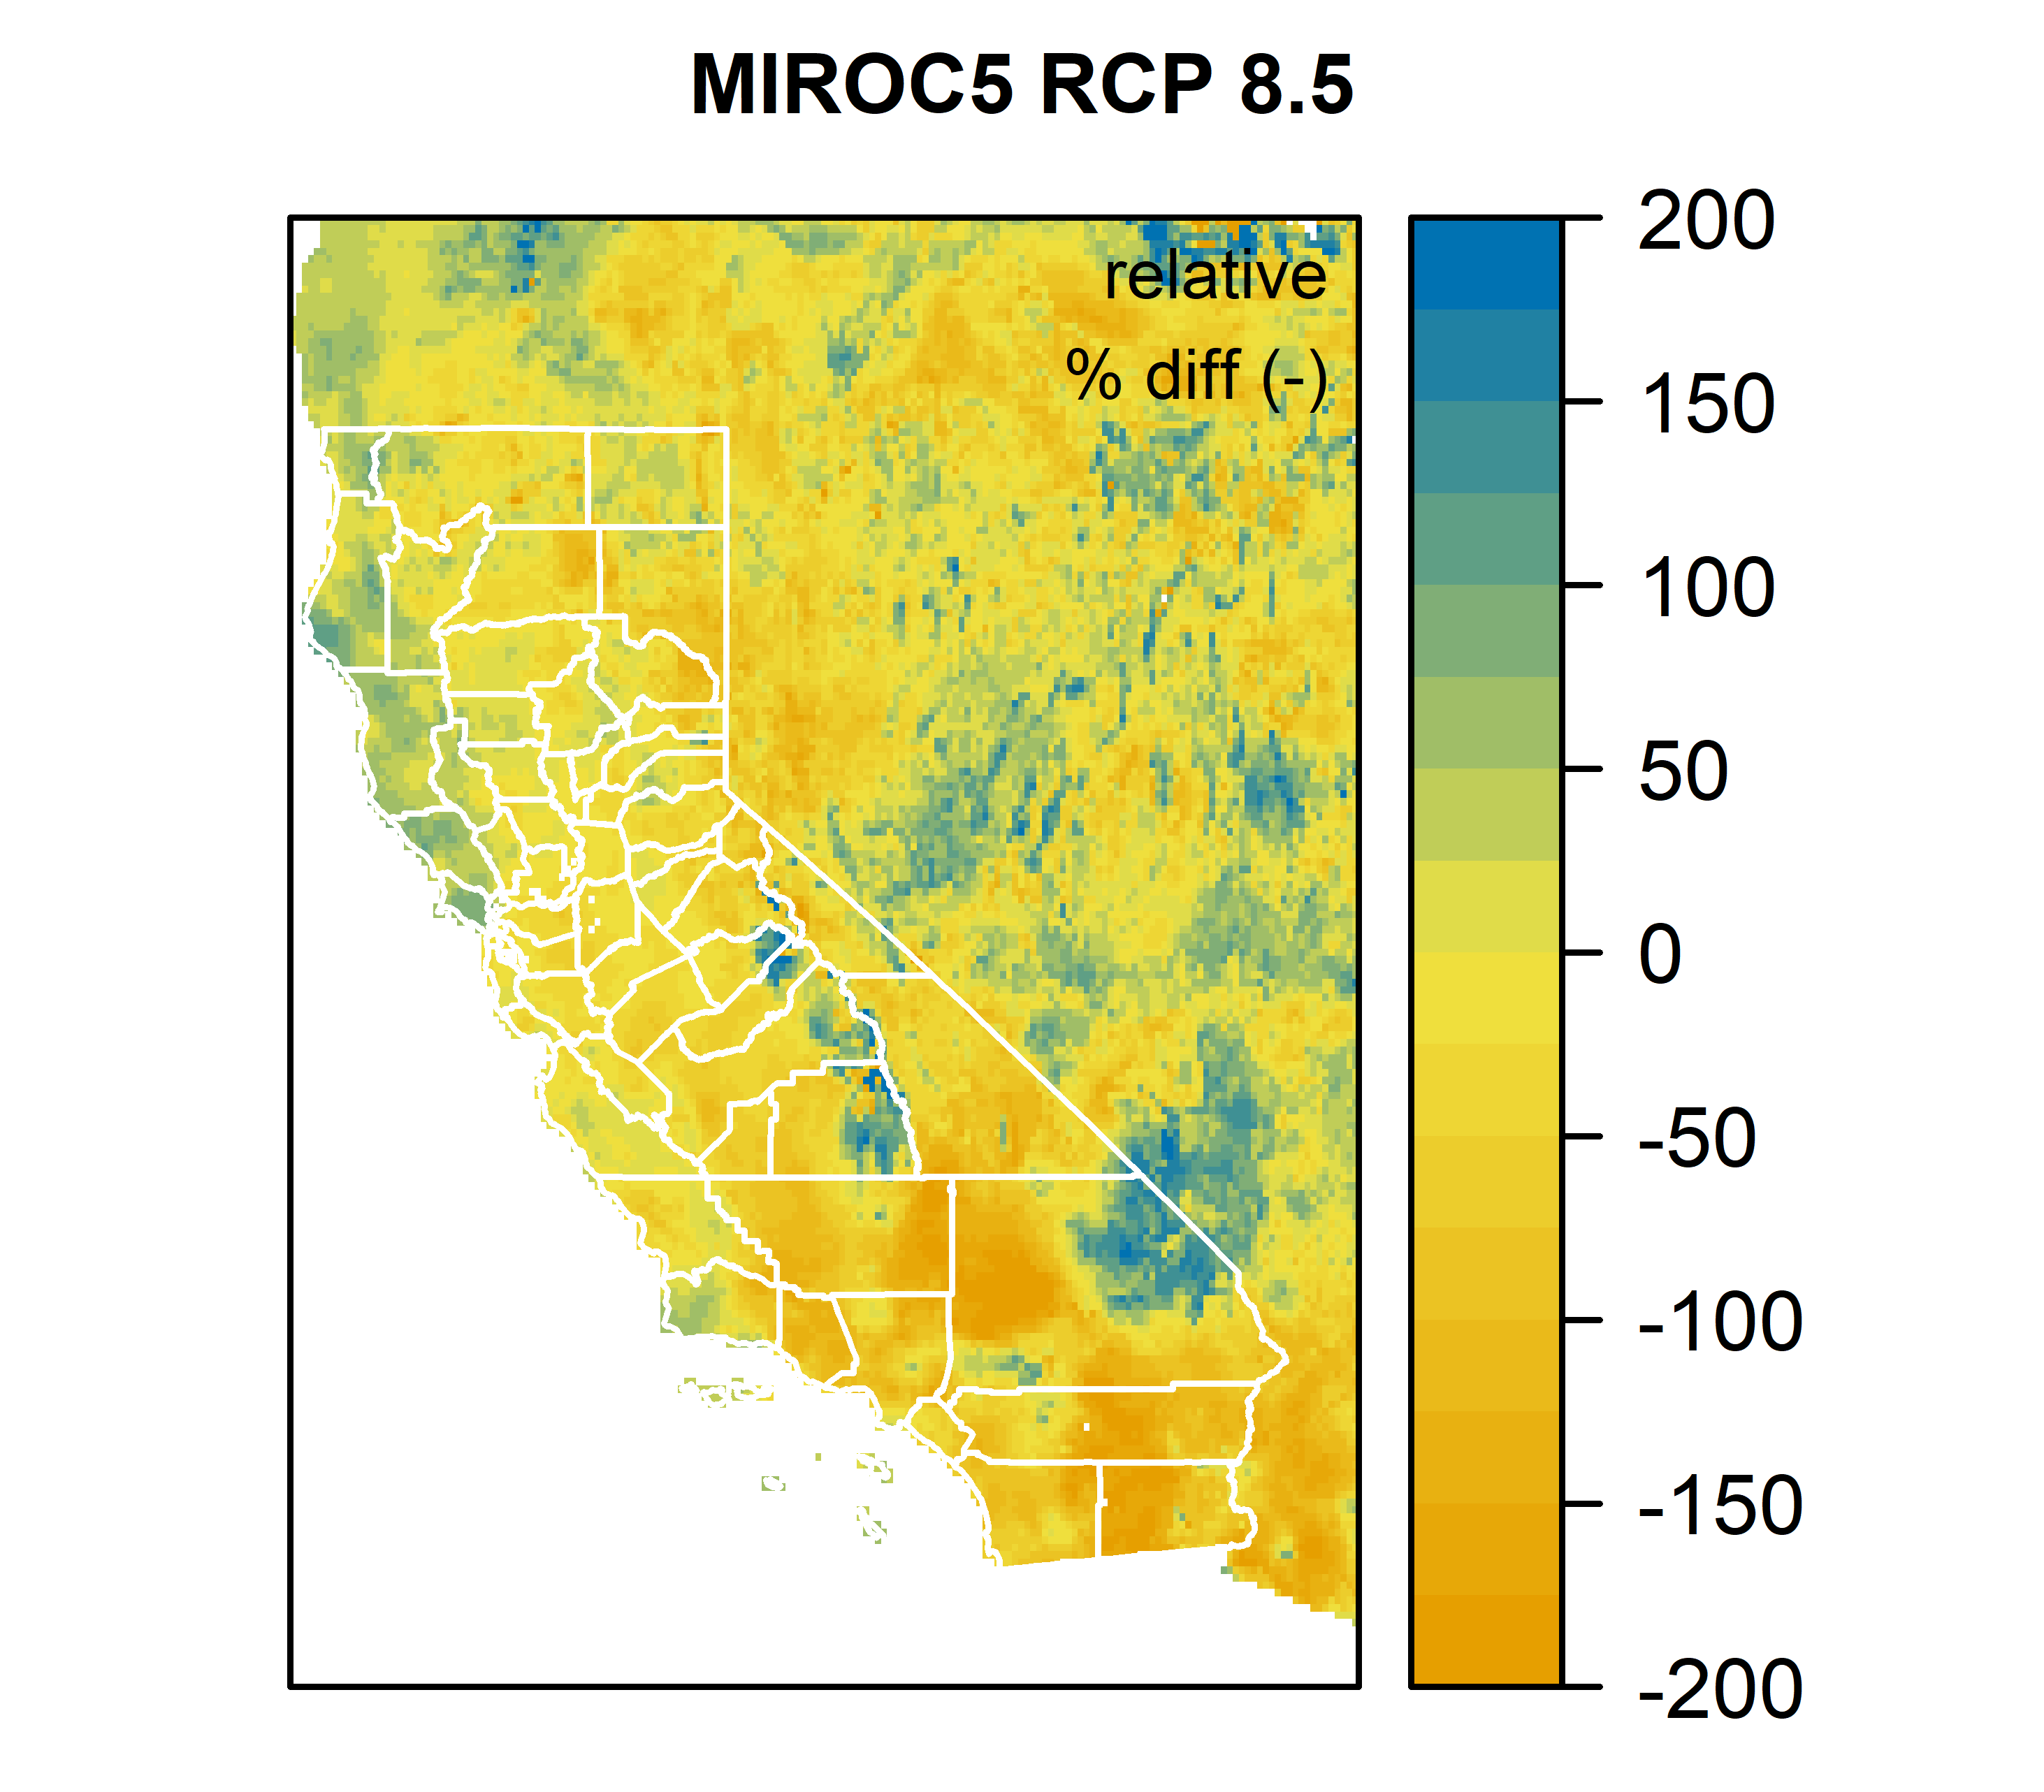
\includegraphics[width=.24\textwidth, trim={1cm 0 0 0}]{plots/rplot54_RNF_MIROC5_85_rpd.png}
    \caption[Relative percent difference in runoff for each climate model.]{Relative percent difference in runoff for each climate model. Much like the changes in precipitation, southern California becomes wetter in CNRMCM5 RCP 4.5 and HadGEM2ES 4.5, and in all models, except for CanESM2, the RCP 8.5 scenario is dryer than its counter part RCP 4.5. MIROC5 RCP 4.5 is most unlike the other models in that it projects a wetter environment for the majority of California (i.e., the central valley and southern California). However, its RCP 8.5 projects a much drier state.}
    \label{fig:rpdmap_rnf}
\end{figure}

Figure \ref{fig:rpd_var} compares the mean RPD in precipitation, temperature, and runoff for different GCMs. These values were calculated by: taking a 30 year subset of the annual values for the projected data (2070-2099) and the observed (1976-2005); finding the RDP for each year (with 1-to-1 matching: 2070 with 1976, 2071 with 1977, etc.); cropping these rasters to the California boundary; averaging the RDPs for each pixel across time; and averaging across space to arrive at one mean RDP for each GCM and RCP combination. Figure \ref{fig:rpd_var}(a) shows that models with RCP 8.5, on average, project hotter climates. The CanESM models and the CNRMCM5 RCP 8.5, on average, project wetter climates. Using these models can give us a wide range of possible futures (dry/wet, and warm/less warm) for California. Figure \ref{fig:rpd_var}(b) shows that runoff in all models generally increases linearly with precipitation and at a higher rate, confirming the positive relationship used when constructing runoff. 
 
\begin{figure}
	\centering
	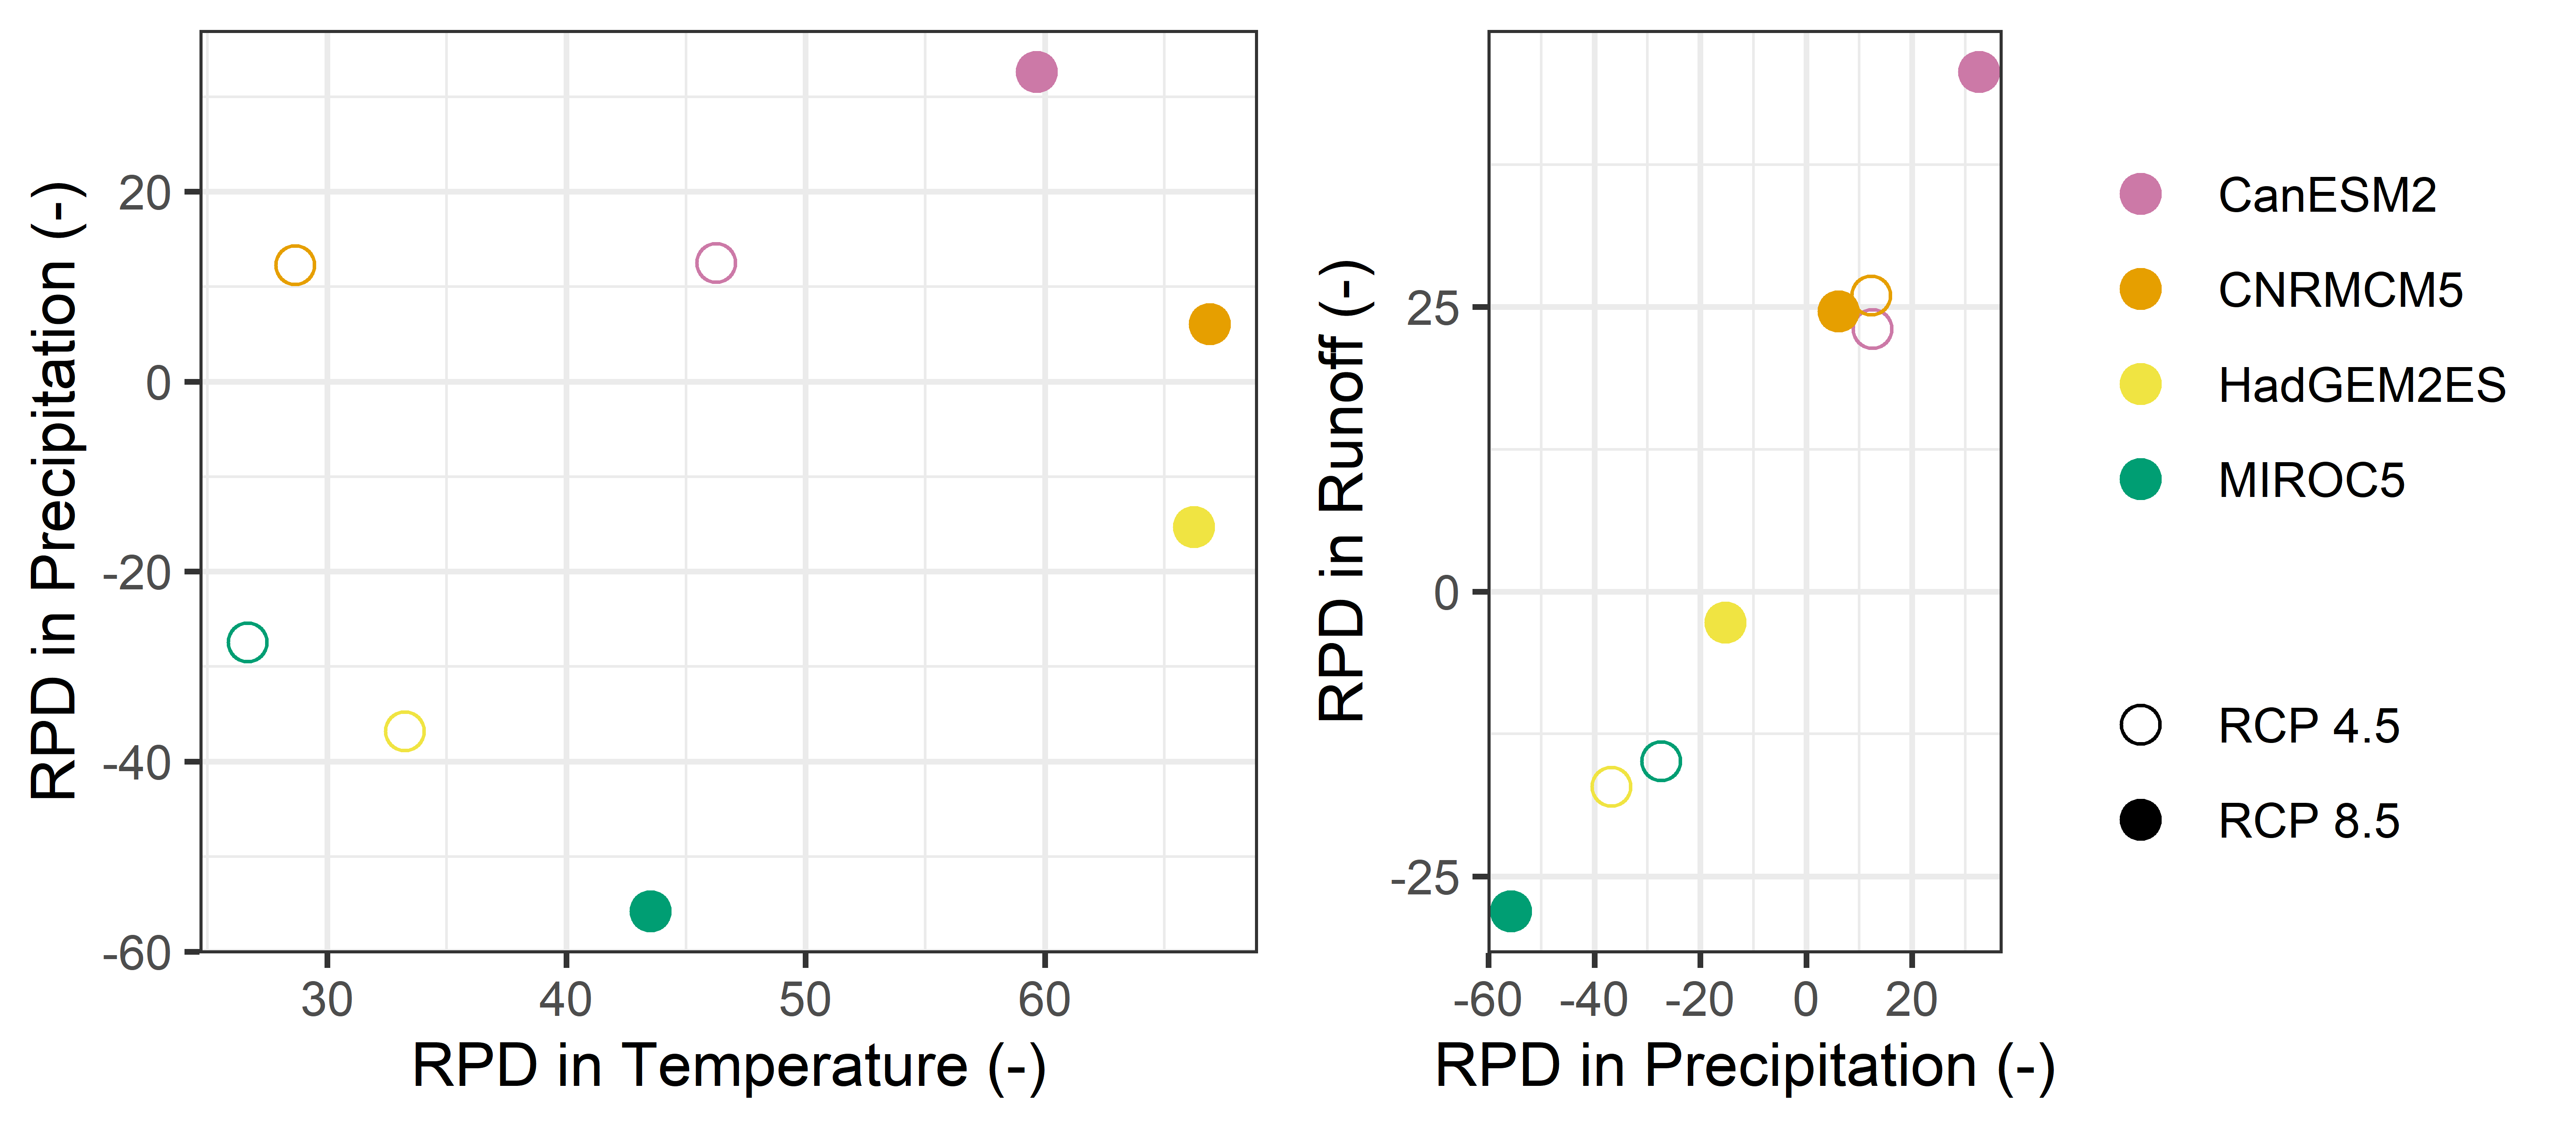
\includegraphics[width=\textwidth,trim={0 0 0 0},clip=true]{plots/rplot56_relperdiff_all.png}
	\caption[Relative percent difference in precipitation, temperature, and runoff for different GCMs.]{Relative percent difference in precipitation, temperature, and runoff for different GCMs. (a) Models with RCP 8.5, on average, project hotter climates. The CanESM models and the CNRMCM5 RCP 8.5, on average, project wetter climates. (b) Runoff in all models generally increases linearly with precipitation and at a higher rate.}
	\label{fig:rpd_var}
\end{figure}

Figure \ref{fig:obscc_var} shows the mean annual precipitation, temperature, and runoff over time. These values were calculated by averaging the parameter value across California and Nevada for each year. With uncertainty in models, scenarios, and climate there are many varied projection paths these variables can take. MIROC 5 RCP 4.5 and CNRMCM5 RCP 4.5 project a wetter climate (confirming mapped values in Figure \ref{fig:rpdmap_rnf}). Annual temperature values slightly increase over time in all models with RCP 4.5 values generally lower than RCP 8.5.  Runoff shows more of a change compared to precipitation, with more frequent peaks in the projections compared to the observed. 

\begin{figure}
	\centering
	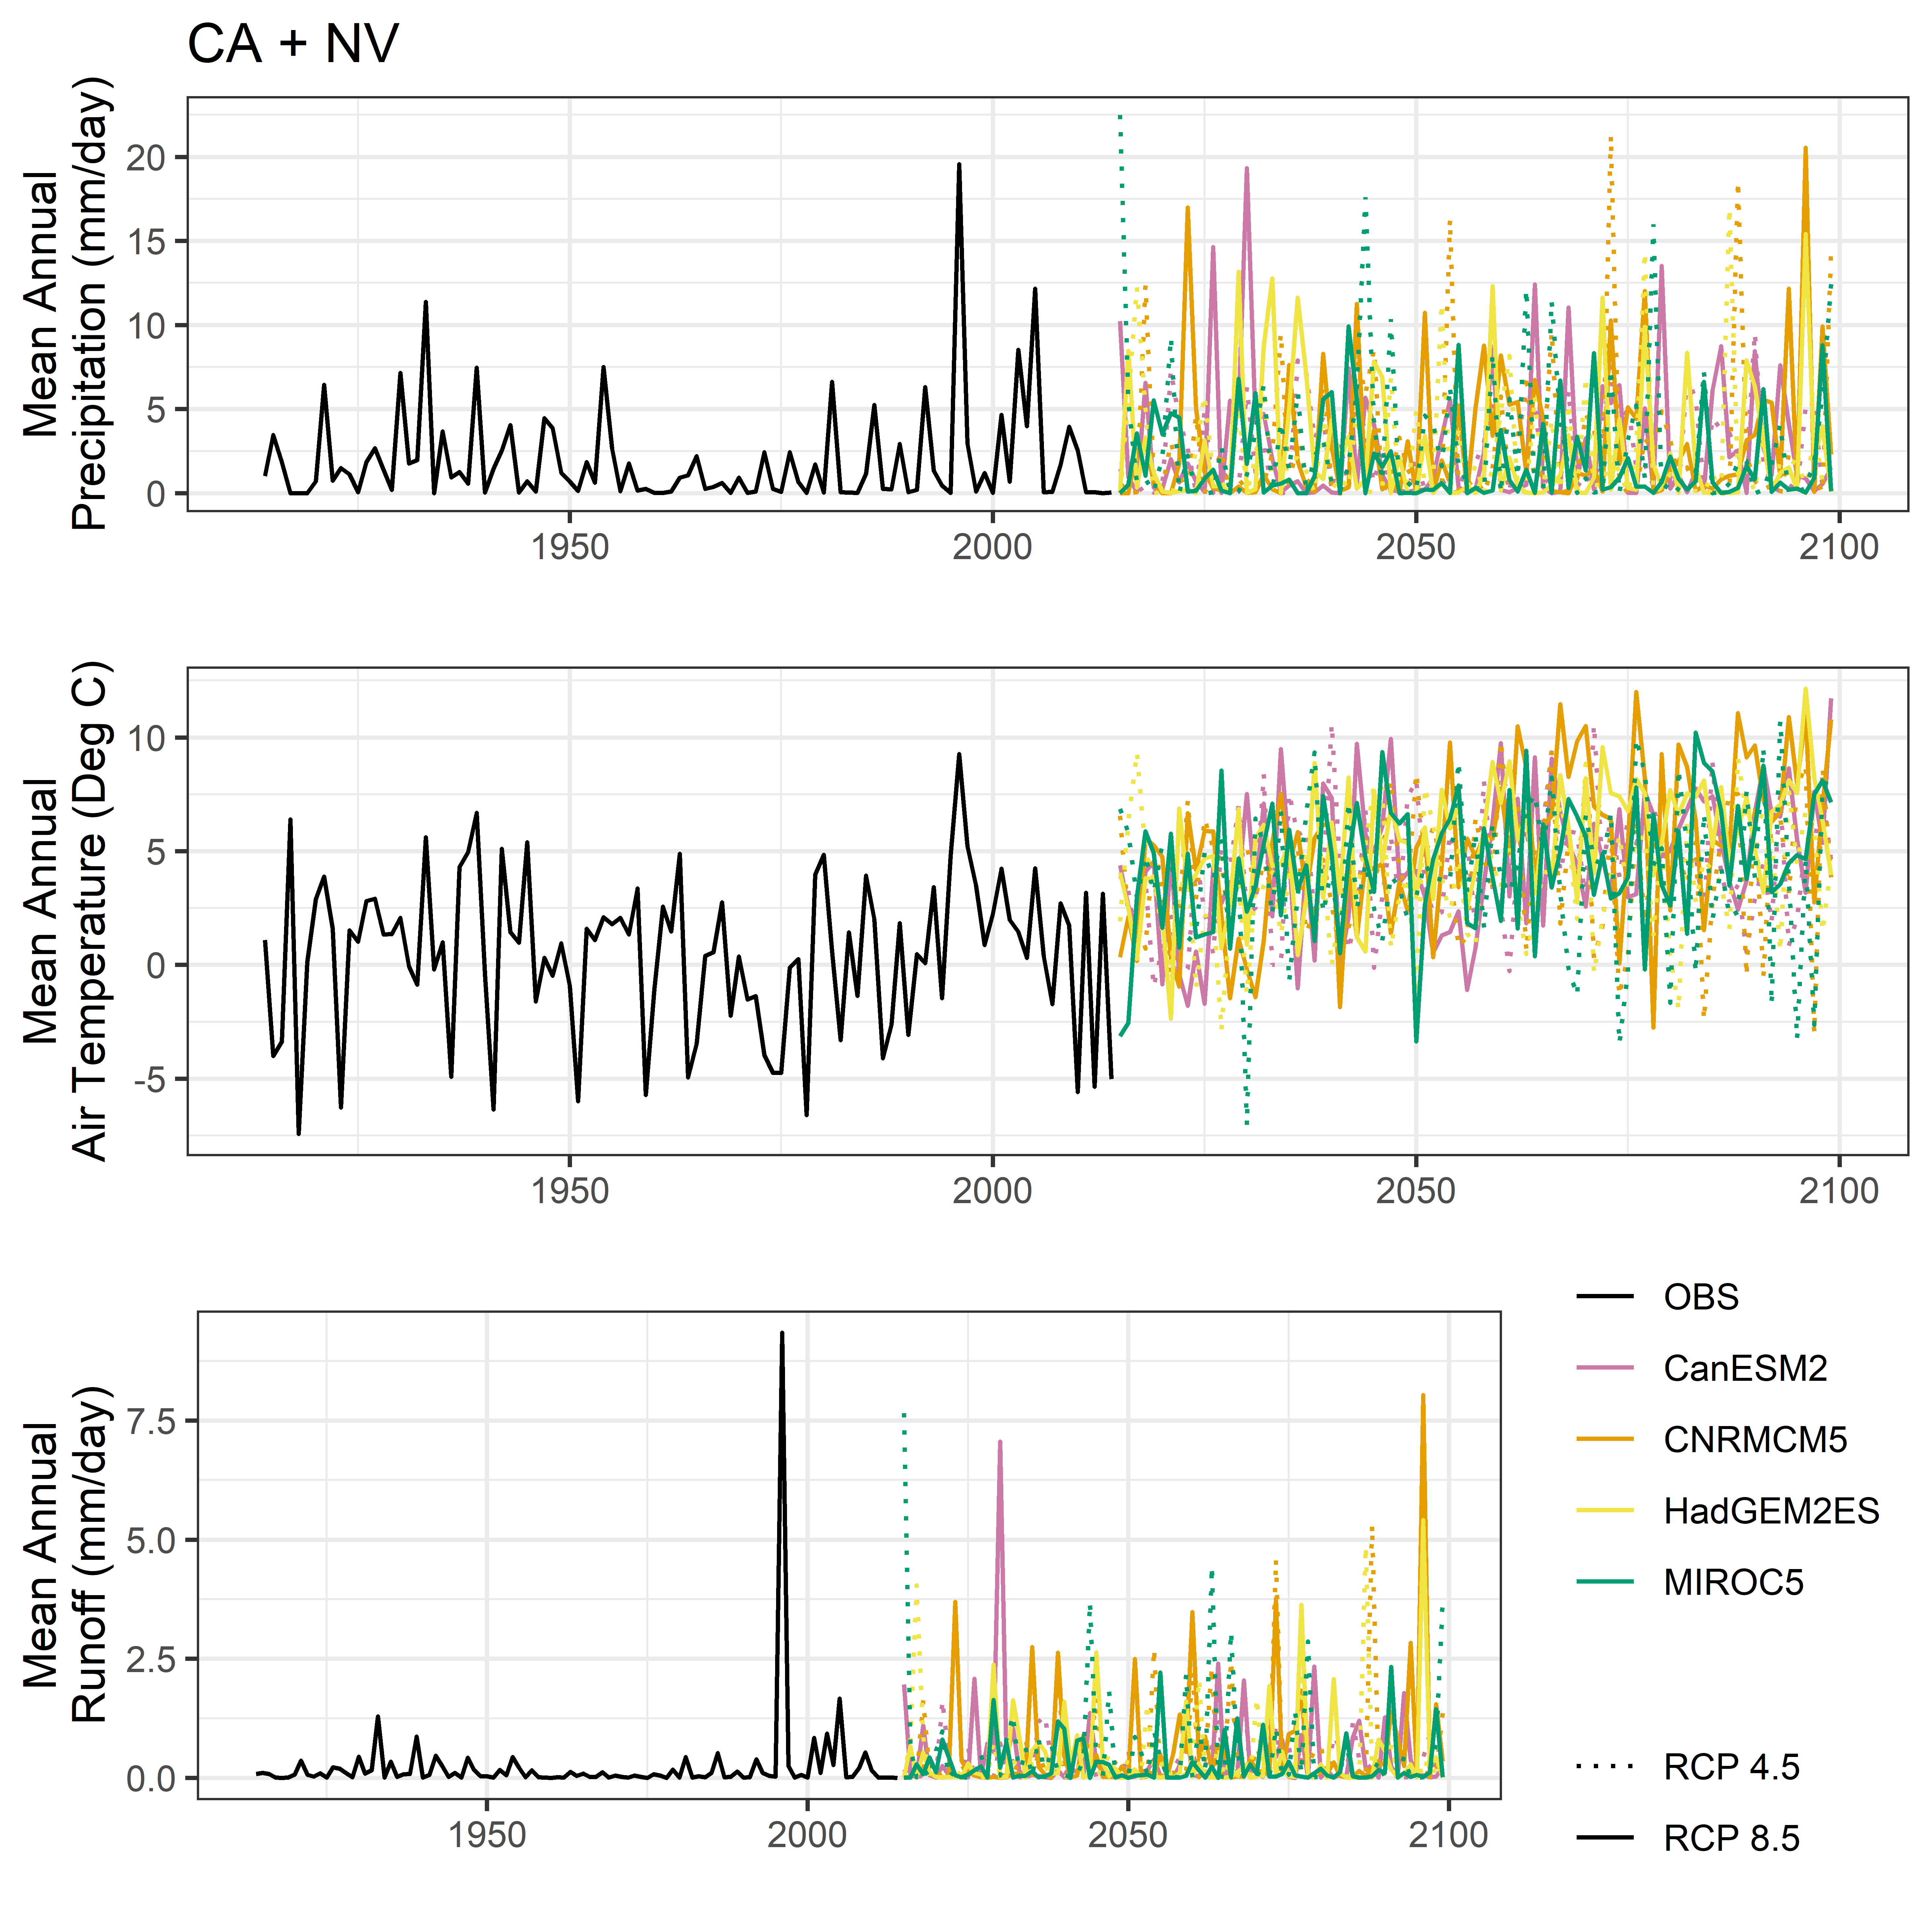
\includegraphics[width=\textwidth, trim={0 0 0 0}, clip=true]{plots/rplot55_obscc_all.png}
	\caption[Time series of projections in precipitation, temperature, and runoff.]{Time series of projections in precipitation, temperature, and runoff. MIROC 5 RCP 4.5 and CNRMCM5 RCP 4.5 project a wetter climate. Annual temperature values slightly increase over time in all models with RCP 4.5 values generally lower than RCP 8.5. Runoff seems to show more of a change compared to precipitation, with more frequent higher values in the projections compared to the observed.}
	\label{fig:obscc_var}
\end{figure}

To smooth out Figure \ref{fig:obscc_var}, Figures \ref{fig:rollmean_var} and \ref{fig:rollsd_var} show the rolling 10 year mean and standard deviations in annual precipitation, temperature, and runoff. These values were calculated by: first, taking a 10 year rolling window starting from 2015 and looking forward in time; finding the average or the standard deviation of the annual parameter values for each raster pixel in time with the last 10 years (2090-2099) discarded from the analysis; finding the spatial mean of the 10 year rolling mean or standard deviation for each parameter. Figure \ref{fig:rollmean_var} shows mean precipitation increasing in CNRMCM5 RCP 8.5. Mean temperature increases in most models and is more pronounced in RCP 8.5. Mean runoff follows mean precipitation trends. Figure \ref{fig:rollsd_var} shows standard deviations in precipitation increasing in CNRMCM5 RCP 8.5 and HadGEM2ES RCP 8.5. Standard deviation in temperature increase in MIROC5 RCP 4.5 and CNRMCM5 RCP 4.5. Standard deviations in runoff follows the trends seen in precipitation. In all but CNRMCM5 RCP 8.5 (cool/wet model), the differences in precipitation and runoff across models are evident from the beginning of the time period and the mean and standard deviations remain stationary. 

\begin{figure}
	\centering
	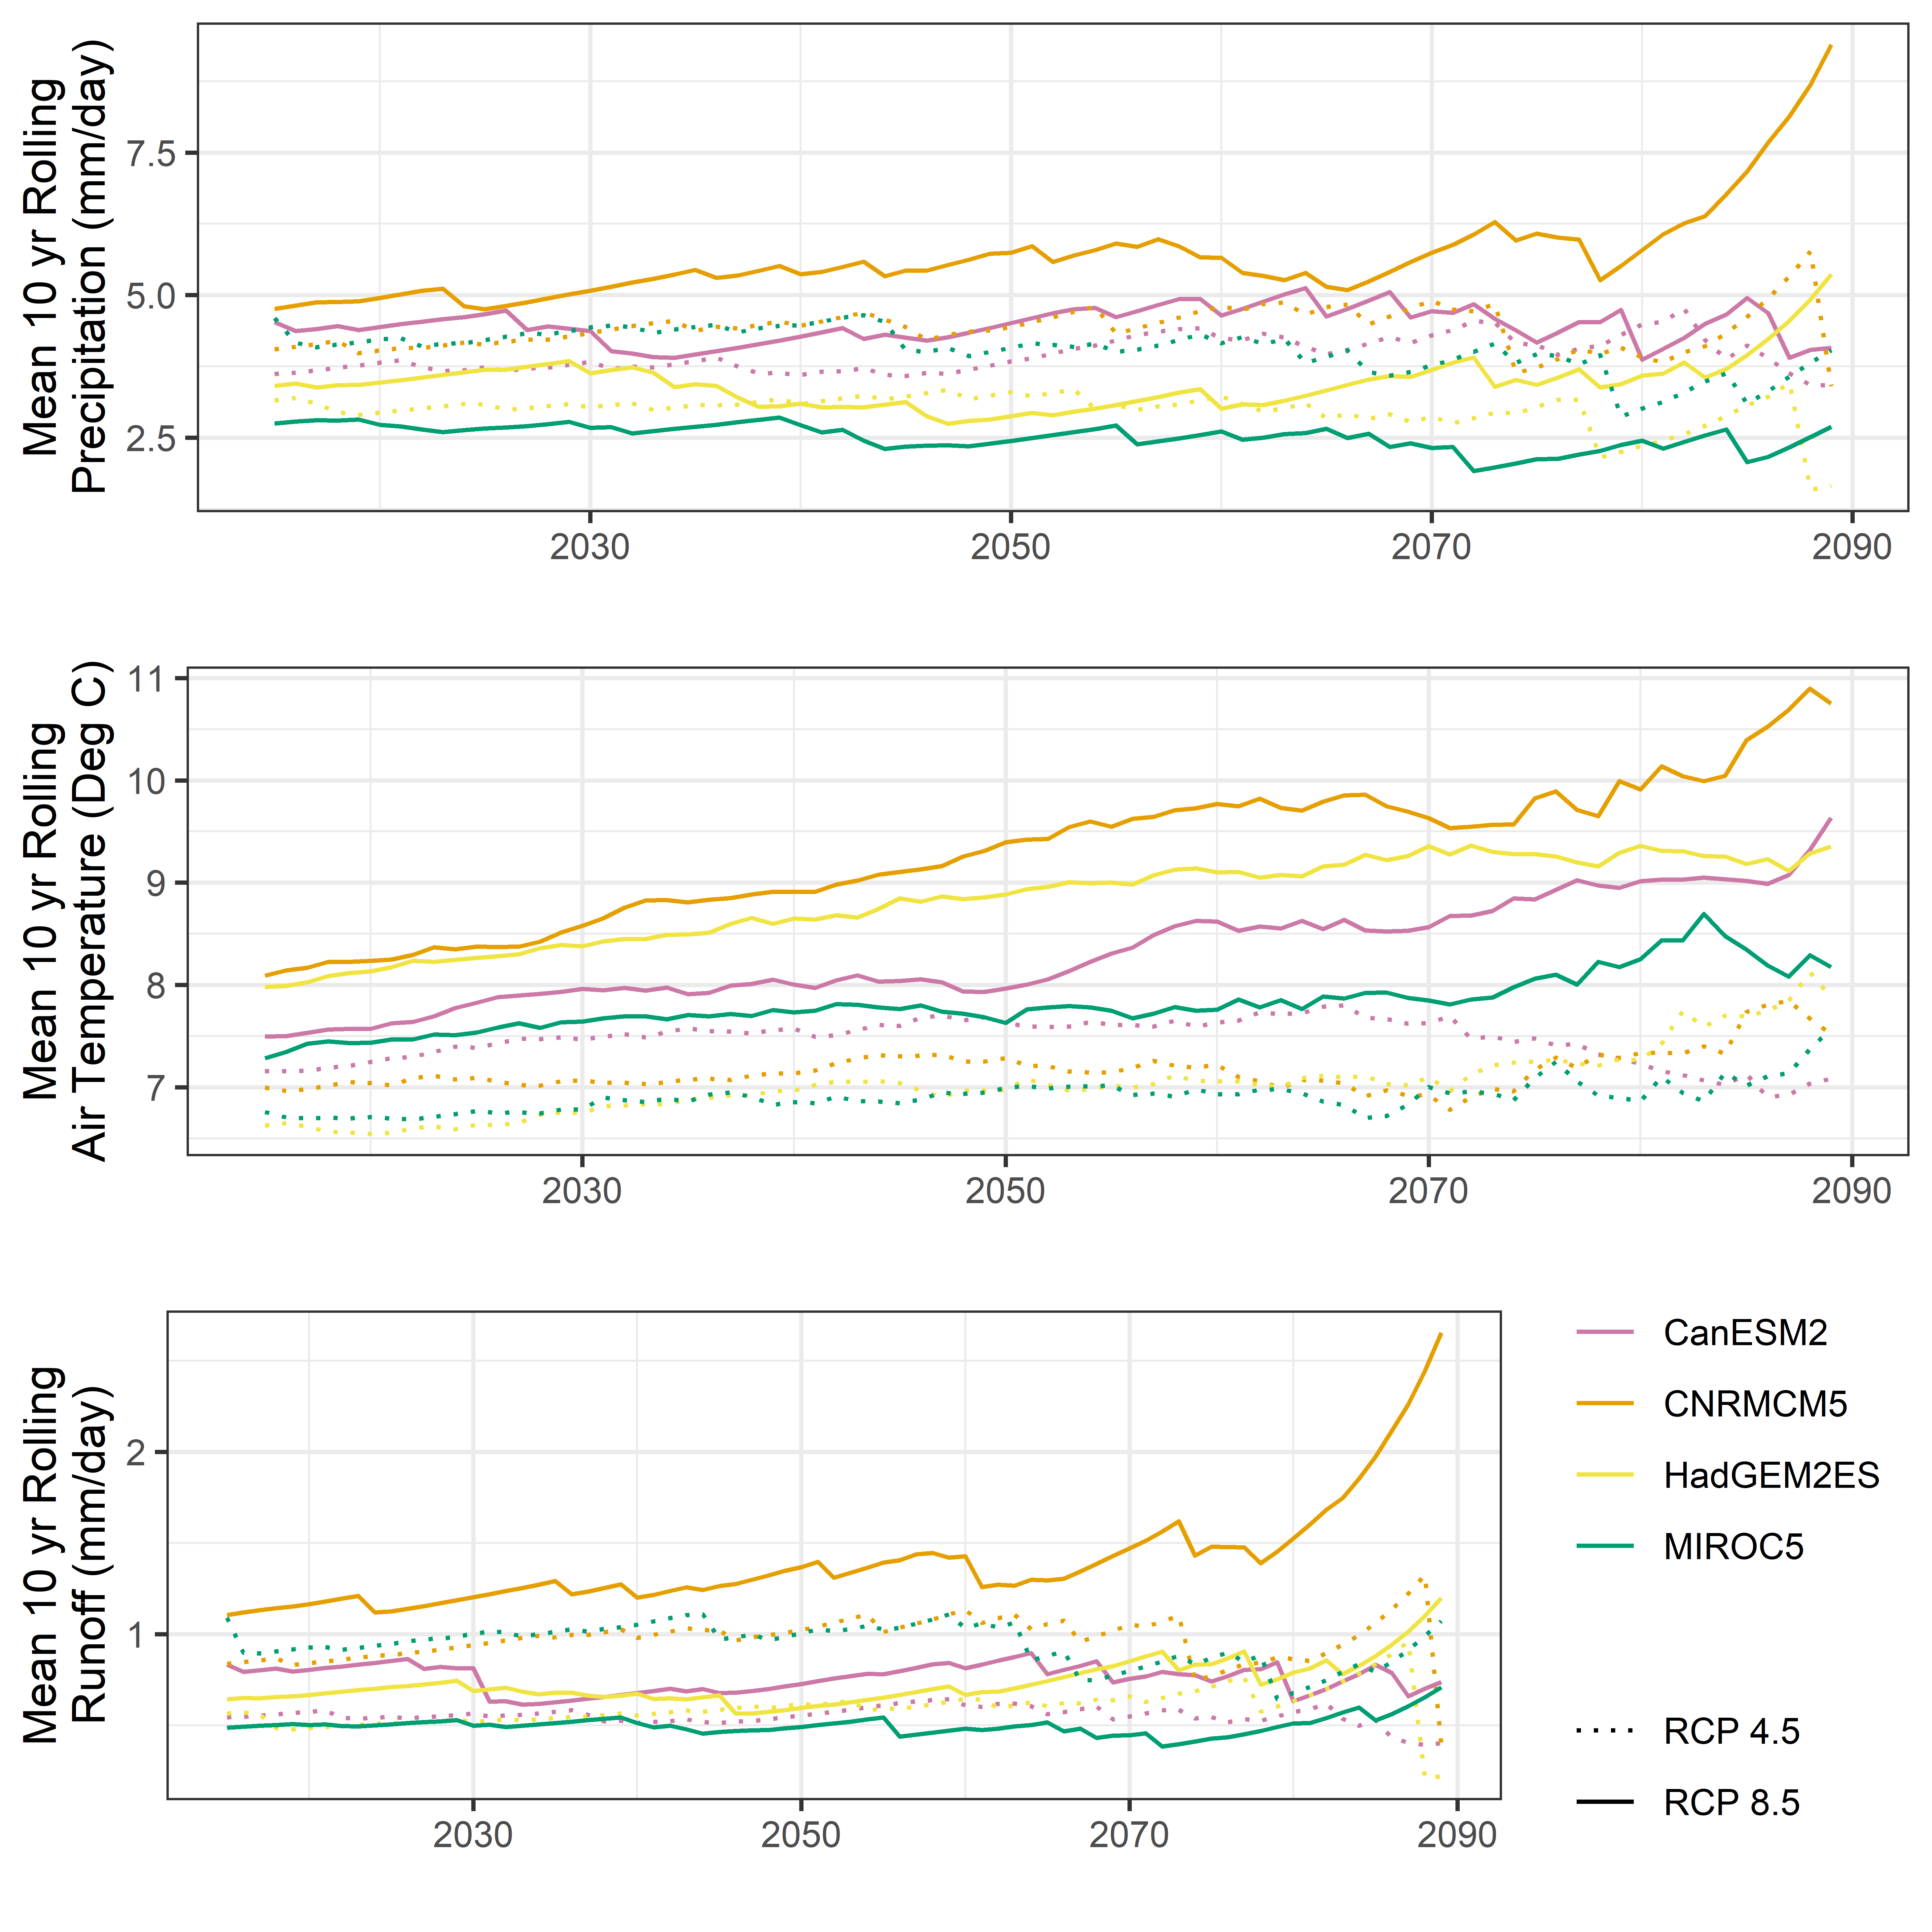
\includegraphics[width=\textwidth, trim={0 0 0 0}, clip=true]{plots/rplot57_rollmean_all.png}
	\caption[Time series of 10 year rolling mean in precipitation, temperature, and runoff.]{Time series of 10 year rolling mean in precipitation, temperature, and runoff. Most differences in precipitation between models is in the mean precipitation rather than in trends, except in CNRMCM5 RCP8.5 (cool/wet model). Mean temperature increases in most models and is more pronounced in RCP 8.5. Mean runoff follows the trends seen in mean precipitation.}
	\label{fig:rollmean_var}
\end{figure}

\begin{figure}
	\centering
	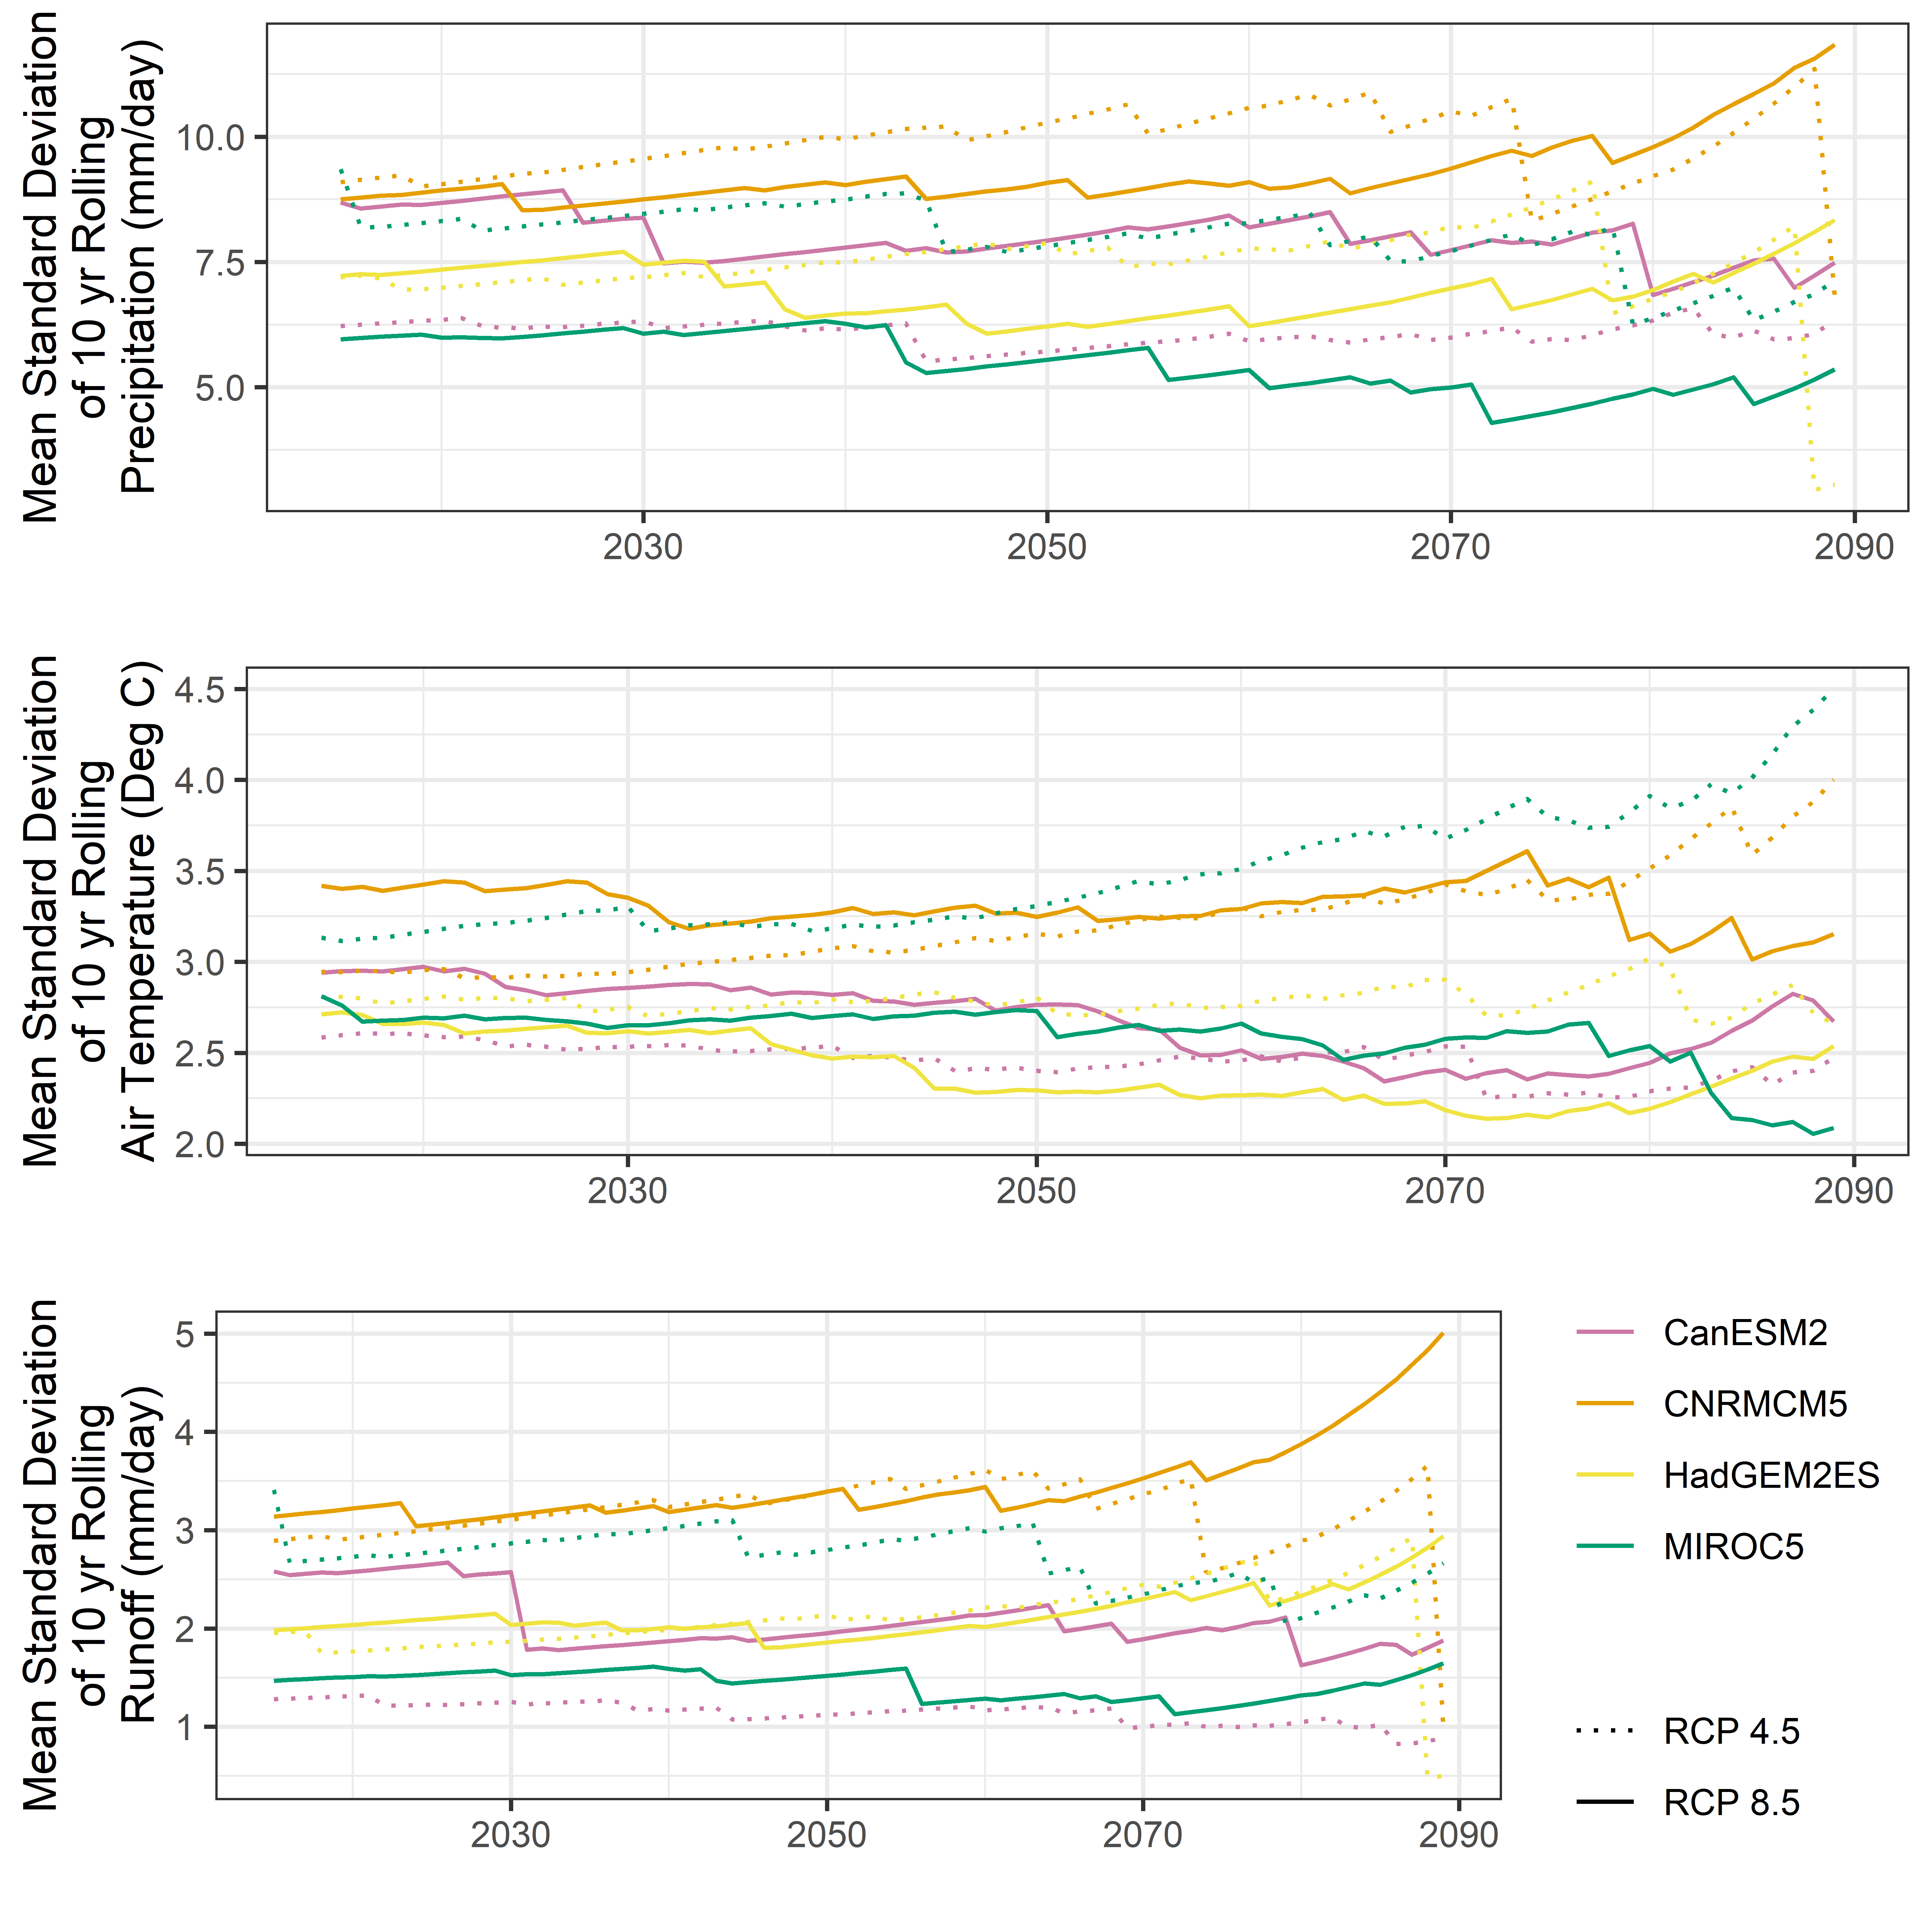
\includegraphics[width=\textwidth, trim={0 0 0 0}, clip=true]{plots/rplot57_rollsd_all.png}
	\caption[Time series of 10 year rolling standard deviation in precipitation, temperature, and runoff.]{Time series of 10 year rolling standard deviation in precipitation, temperature, and runoff. Standard deviations in precipitation increase in CNRMCM5 RCP 8.5 (cool/wet model) and HadGEM2ES RCP 8.5 (the warm/dry model). Standard deviation in temperature increase in MIROC5 RCP 4.5 and CNRMCM5 RCP 4.5. In RCP 4.5, the standard deviations decrease at the end of the century. Again, standard deviations in runoff follows trends seen in precipitation.}
	\label{fig:rollsd_var}
\end{figure}

%-----------------------------------------------------------------------------------------------------------------------------------------------------------------------------------------------------
\section{Methods}
Each downscaled climate change model data is put through the NN model built on past hydrology and the model predictions are compared to the climate model projections. The climate model projections come in raster (i.e., not routed) format. A simple aggregation to basin boundaries finds the mean precipitation (and its lagged values), mean temperature (and its lagged values), mean snow, and total runoff over the basin. One problem with this simple routing technique is that some end-of-month storms may end up as streamflow in the next month; some precipitation values are getting counted in the month that the flows it generates is not. Since, the model is on a monthly time-step we will ignore this small accounting difficulty. The other option was to use the Variable Infiltration Capacity (VIC) routed streamflows that do account for basin lags, however, this dataset was only developed for 11 basins, hand selected for the CALSIM II model's major reservoir inflow locations. To keep all our 67 diverse basins in the study we will use the aforementioned aggregation method as a good approximation for routing. 
 
%-----------------------------------------------------------------------------------------------------------------------------------------------------------------------------------------------------
\section{Results}
Figure \ref{fig:modcomp} shows the NN model predictions compared to climate model projections for unaggregated monthly data for each basin. There is fairly good agreement between the purely statistical (NN) and the mechanistic models (GCMs) with the highest R\textsuperscript{2} of 0.72 belonging to the CanESM2 and CNRMCM5 models. In all models the NN is slightly biased to predict higher values compared to the climate change models as is evident in the slope of the best fit line ($\beta_1>1$). 

\begin{figure}
	\centering
	\includegraphics[width=\textwidth,trim={0 0 0 0},clip=true]{plots/rplot52_obsvspred.png}
	\caption[NN model predictions compared to climate model projections.]{NN model predictions compared to climate model projections (monthly data for each basin). There is fairly good agreement between the purely statistical (the NN) and the mechanistic models (the climate change models) with the highest R\textsuperscript{2} being 0.72 for the CanESM2 and CNRMCM5 RCP 4.5 models.} 
	\label{fig:modcomp}
\end{figure}

Figure \ref{fig:density} shows the probability densities for the monthly NN unimpaired flow predictions and the climate model runoff projections. Similar to results in previous chapters, the NN model predicts fewer low flows compared to the runoff from climate models. There is very little difference in the densities across the various climate data in either the NN model prediction or runoff projections from the climate models themselves. Also, there is very little difference observed across the two RCPs. This shows that our simple routing precipitation to runoff eliminates the differences across models and should be replaced with a better model (e.g., VIC). 

\begin{figure}
	\centering
	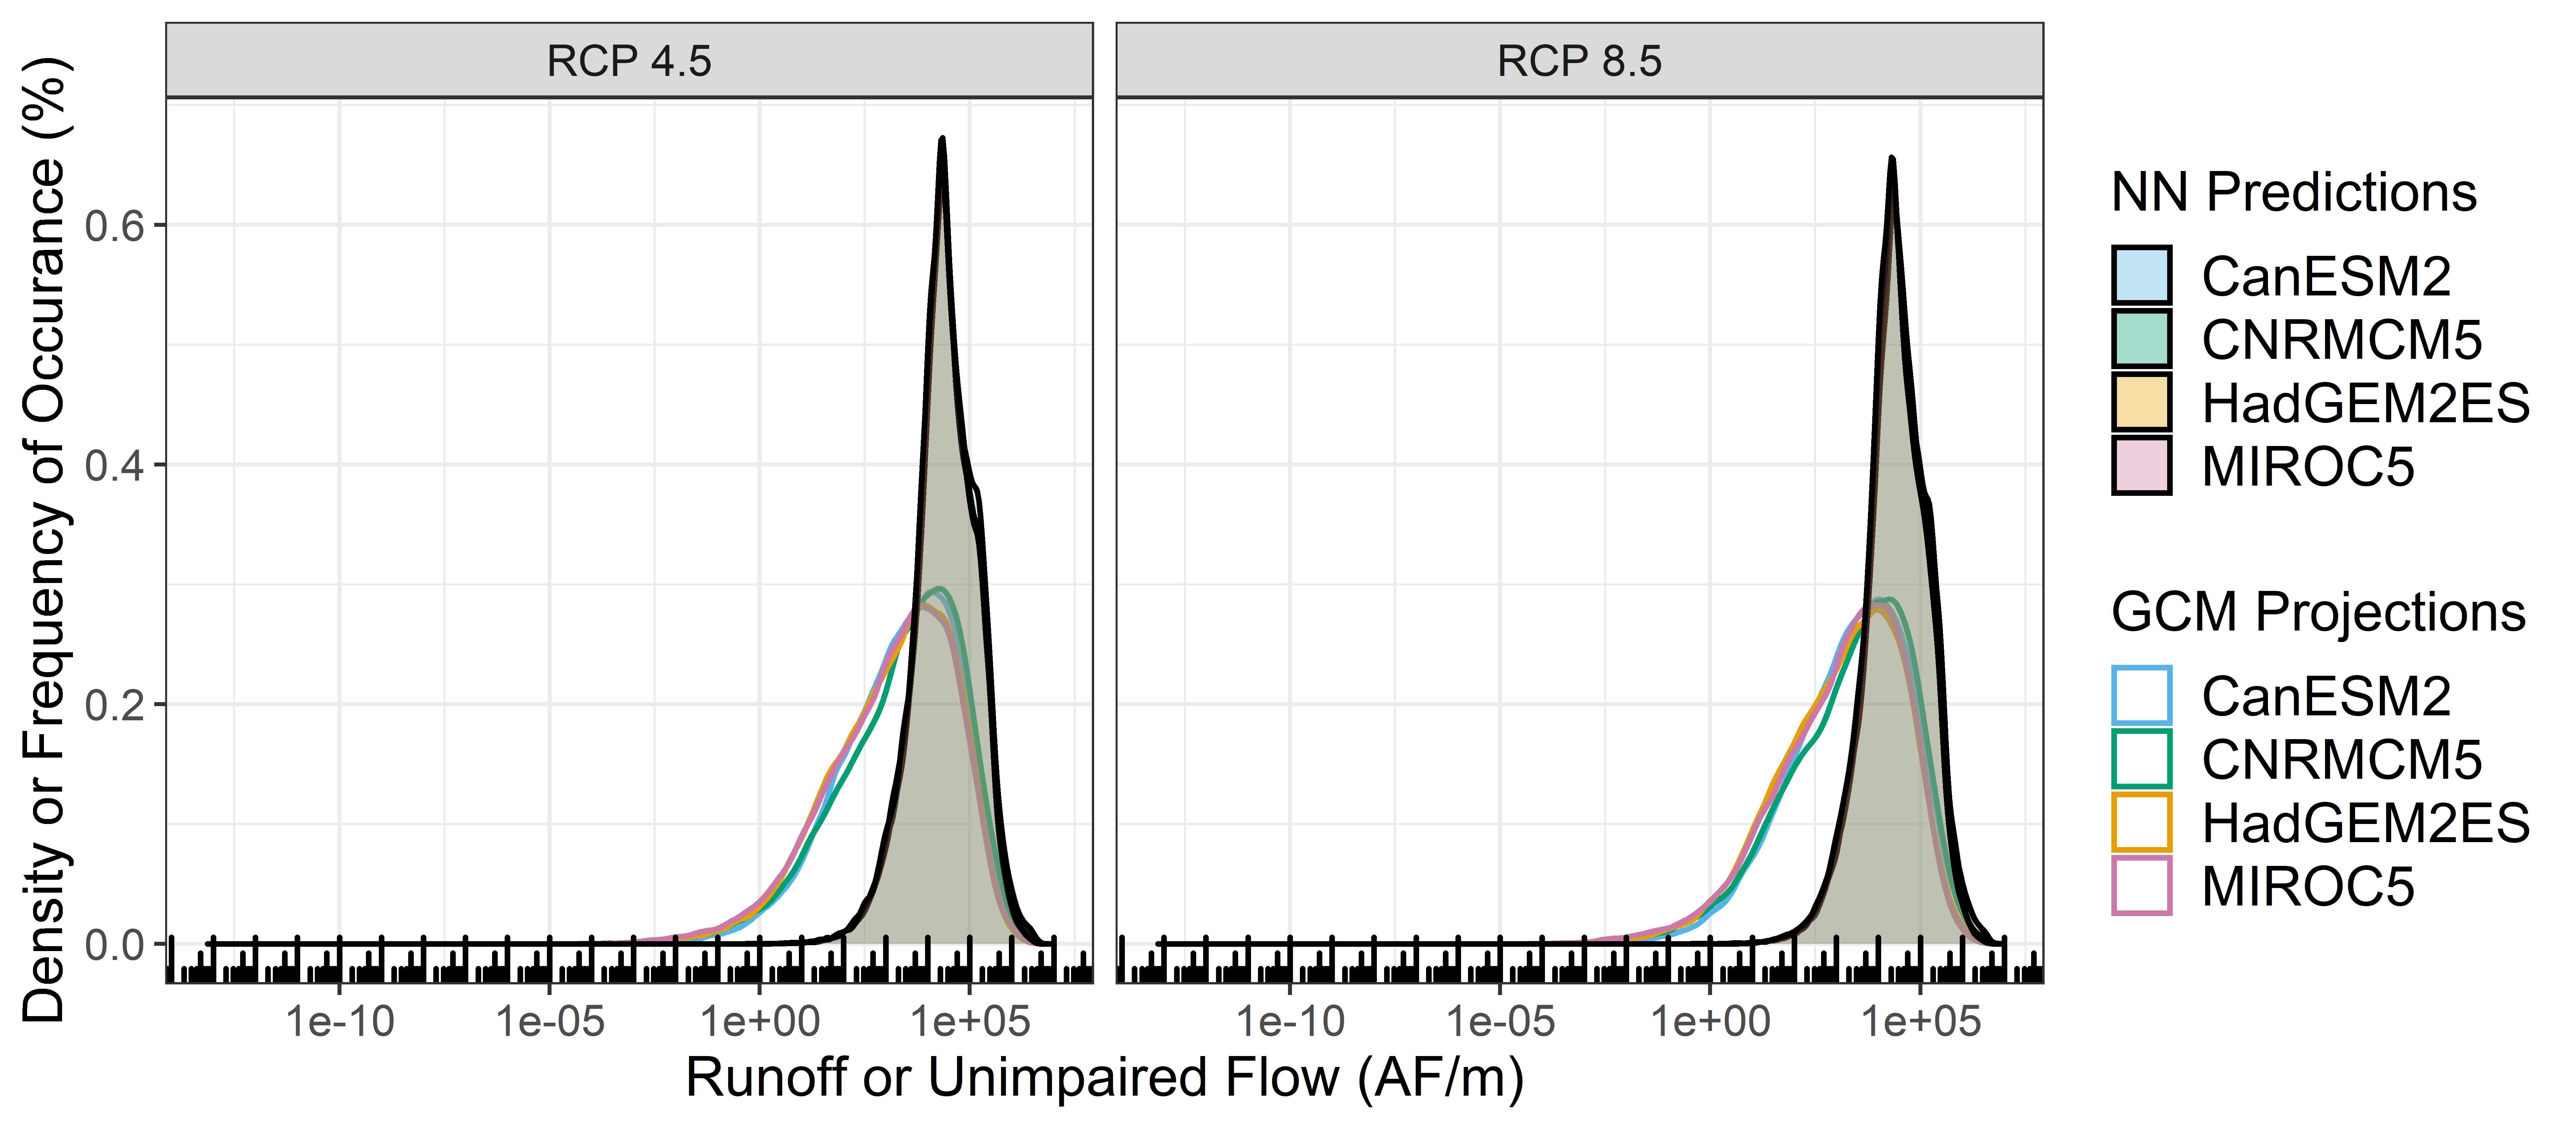
\includegraphics[width=\textwidth,trim={0 0 0 0},clip=true]{plots/rplot53_density.png}
	\caption[Predicted unimpaired flow density compared to runoff densities from GCMs.]{Predicted unimpaired flow density compared to runoff densities from GCMs. The NN model does not capture low flows like climate models. There is very little difference in the densities across the various climate data in either the NN model prediction or runoff projections from the climate models themselves. Also, there is very little difference observed across the two RCPs.} 
	\label{fig:density}
\end{figure}

Figures \ref{fig:camean_monthly_comp}, \ref{fig:camean_annual_comp}, and \ref{fig:camean_10yr_comp} compare the monthly, moving 1 year average, and moving 10 year average NN model predictions with climate model runoff projection. Instead of showing each basin separately, this plot shows the mean flows across the 67 basins. The moving window allows us to view larger trends. Unsurprisingly, as the window grows larger, the values are ``smoothed out'', and the agreement (in terms of R\textsuperscript{2}) increases. For example, in the CNRMCM5 RCP 4.5 R\textsuperscript{2} increases from 0.77, to 0.90, and 0.96 when comparing monthly, moving 1 year average, and moving 10 year average values. However, with the increase in R\textsuperscript{2} the NN model biases increase as well. For example, the slope of the best fit line in CNRMCM5 RCP 4.5 increases from 0.95 to 1.44 and 1.74. This is due to the NN model's inability to capture a higher density at the lower flows, which was observed in Figure \ref{fig:density}.

\begin{figure}
	\centering
	\includegraphics[width=\textwidth,trim={0 0 0 0},clip=true]{plots/rplot58_camean_monthly_comp2.png}
	\caption[Mean California unimpaired flow NN model predictions vs. climate model projections (monthly data).]{Mean California unimpaired flow NN model predictions vs. climate model projections (monthly data). There is fairly good agreement between the two types of models on the average California flows. Compared to unaggregated monthly data model agreement slightly increases as the data gets aggregated across California.} 
	\label{fig:camean_monthly_comp}
\end{figure}

\begin{figure}
	\centering
	\includegraphics[width=\textwidth,trim={0 0 0 0},clip=true]{plots/rplot58_camean_annualrolling_comp2.png}
	\caption[Mean California unimpaired flow NN model predictions vs. climate model projections (annual moving average data).]{Mean California unimpaired flow NN model predictions vs. climate model projections (annual moving average data). There is fairly good agreement between the two types of models on the average California flows. Compared to monthly data, here, model agreement increases slightly.} 
	\label{fig:camean_annual_comp}
\end{figure}

\begin{figure}
	\centering
	\includegraphics[width=\textwidth,trim={0 0 0 0},clip=true]{plots/rplot58_camean_10yr_rolling_comp2.png}
	\caption[Mean California unimpaired flow NN model predictions vs. climate model projections (10 year moving average data).]{Mean California unimpaired flow NN model predictions vs. climate model projections (10 year moving average data). There is fairly good agreement between the two types of models on the average California flows. Compared to 1 year moving average data, here, model agreement increases slightly but so does biases (slope of the best fit line).} 
	\label{fig:camean_10yr_comp}
\end{figure}

Figures \ref{fig:camean_monthly_comp_ts}, \ref{fig:camean_annual_comp_ts}, and \ref{fig:camean_10yr_comp_ts} confirm the NN model's bias observed in the previous plots. Here, the monthly, moving 1 year average, and moving 10 year average NN model predictions and climate model runoff projections are plotted through time. As the window grows larger the NN model predictions increase as compared to the climate model predictions. This is again due to the NN model's inability to capture a higher density at the lower flows, which was observed in Figure \ref{fig:density}.

\begin{figure}
	\centering
	\includegraphics[width=\textwidth,trim={0 0 0 0},clip=true]{plots/rplot58_camean_monthly_comp.png}
	\caption[Mean California unimpaired flow climate model and NN model comparisons in time (monthly data).]{Mean California unimpaired flow climate model and NN model comparisons in time. The NN model captures the high flow events at the right time but is slightly under predicting them compared to the climate model projections.} 
	\label{fig:camean_monthly_comp_ts}
\end{figure}

\begin{figure}
	\centering
	\includegraphics[width=\textwidth,trim={0 0 0 0},clip=true]{plots/rplot58_camean_annualrolling_comp.png}
	\caption[Mean California unimpaired flow climate model and NN model comparisons in time (annual moving average data).]{Mean California unimpaired flow climate model and NN model comparisons in time (1 year moving average data). The NN model's predictions over-take the climate model projections.} 
	\label{fig:camean_annual_comp_ts}
\end{figure}

\begin{figure}
	\centering
	\includegraphics[width=\textwidth,trim={0 0 0 0},clip=true]{plots/rplot58_camean_10yr_rolling_comp.png}
	\caption[Mean California unimpaired flow climate model and NN model comparisons in time (10 year moving average data).]{Mean California unimpaired flow climate model and NN model comparisons in time (10 year moving average data).The NN model's predictions over-take the climate model projections and a larger moving window means larger differences.} 
	\label{fig:camean_10yr_comp_ts}
\end{figure}

%-----------------------------------------------------------------------------------------------------------------------------------------------------------------------------------------------------
\section{Conclusion}
This chapter used four global climate models with two RCPs each to estimate future hydrology. The climate variable from these models give a wide range of possible futures for California. Some models like the MIROC5 RCP 4.5 and CNRMCM5 RCP 4.5 project a wetter California while most other models project a drier climate in terms of precipitation. Most models agree that in both RCPs, temperatures will rise and are projected to increase 2-4 $^{\circ}$C for RCP 4.5 and 4-7 $^{\circ}$C for RCP 8.5 \cite{pierce2018climate}. Runoff projections show more floods compared to historical hydrology, but are stationary in their mean and standard deviations in all but one model (CNRMCM5, the cool/wet model). 

Statistical models operate from no apriori knowledge of hydrologic processes, and have to be used with caution when extrapolating beyond the time range they were trained on. There is fairly good agreement in the statistical (NN) model's unimpaired flow predictions and the mechanistic (GCM) model's routed runoff (R\textsuperscript{2}= [0.64-0.72]). However, the NN model does not capture low flows like the climate models and overestimates their values so much so that when we compare more smoothed data (with a moving average window) we can see a bias emerge ($\beta_1$= [0.95-1.84] for CanESM2 RCP 4.5 for example). This can also be seen in the time series comparisons, where with a larger moving average window the NN model's predictions are systematically higher than the climate model projections. 

Both the GCM or NN model projections are untestable, since the ``reality'' we need to test against will be available either too late or never-an unavoidable feature of all hydrological simulation models discussed by \citeA{klemevs1986operational}. We can argue that the GCM model's projections are slightly more reliable since the processes of finding the amount of recharge and runoff for each pixel ($\sim$ 100 km) from precipitation is grounded in hydrology. However, the downscaling to a finer resolution was a statistical process (i.e., LOCA downscaling), and the routing scheme used here was a simple statistical aggregation to basin boundaries. Therefore, even in the GCM projections many approximations are used to arrive at water balance estimates. The advantages of using statistical learning models still remain; they are easier to use, apply, and operationalize. The next chapter will explain some improvement strategies for the NN model. 
